\documentclass{epr400}
\eprtitle{Handwriting robot}
\eprcode{EPR400}
\eprcandidatename{D.R. Braune}
\eprstudentnumber{23539195}
\eprdate{November 2026}
\eprsupervisor{Prof. H.C. Myburgh}
\eprcopynum{Integrated report revision}
\usepackage[hidelinks]{hyperref}
\usetikzlibrary{arrows.meta}

\usepackage{tabularx}
\usepackage{booktabs}
\usepackage{array}
\usepackage{float}
\usepackage{listings}
\usepackage{placeins}
\floatstyle{ruled}
\newfloat{designalgorithm}{htbp}{loa}
\floatname{designalgorithm}{Algorithm}
\newenvironment{designsteps}{\small\begin{enumerate}\setlength{\itemsep}{2pt}\setlength{\parskip}{0pt}\setlength{\topsep}{3pt}}{\end{enumerate}}
\setlength{\headheight}{15pt}
\setlength{\emergencystretch}{1em}
\definecolor{DesignBlue}{RGB}{25,65,105}
\lstdefinestyle{designcode}{basicstyle=\ttfamily\small,breaklines=true,
  columns=fullflexible,keepspaces=true,showstringspaces=false,
  aboveskip=6pt,belowskip=6pt}


\newcounter{designline}
\newenvironment{designpseudo}{\small\setcounter{designline}{0}\begin{list}{}{\setlength{\leftmargin}{2.1em}\setlength{\labelwidth}{1.6em}\setlength{\labelsep}{0.5em}\setlength{\itemsep}{0pt}\setlength{\parsep}{0pt}\setlength{\topsep}{3pt}}}{\end{list}}
\newcommand{\pstate}[2]{\stepcounter{designline}\item[\arabic{designline}:]\hspace*{#1em}#2}
\newcommand{\prequire}[1]{\par\small\noindent\textbf{Require:} #1\par}
\newcommand{\pensure}[1]{\par\small\noindent\textbf{Ensure:} #1\par}


\clubpenalty=10000
\widowpenalty=10000
\displaywidowpenalty=10000

\newcommand{\reportqt}[2]{\par\bigskip\phantomsection\label{#1}\noindent\QualificationTest{#2}\par\medskip}
\newcommand{\resstep}[1]{\par\medskip\noindent\QualificationSection{#1}\par\nobreak\smallskip}
\begin{document}
\maketitlepage
\pagestyle{plain}
\pagenumbering{roman}
\eprsecwithout{Part 1. Preamble}
\vspace*{0.5cm}
%%
%%  Department of Electrical, Electronic and Computer Engineering.
%%  EPR400/2 Final Report - Preamble.
%%  Copyright (C) 2011-2021 University of Pretoria.
%%

This report describes the engineering process followed to complete my final year, which involved creating a handwriting robot to classify and reproduce text in author's handwriting.
\\[2ex]
% Included comment line to break spacing
\textbf{\textit{1. Project proposal and technical documentation}} \newline
This main report contains an unaltered copy of the approved Project Proposal (as Part 2 of the report).

All the code that I developed appears as a separate submission on the AMS.

\textbf{\textit{2. Project history}} \newline
The project was done on my own, with advice from an ex-project student, algorithms and techniques inspired by referenced papers, like classifier structure.
\\[2ex]
% Included comment line to break spacing
\textbf{\textit{3. Language editing}} \newline
This document has been language edited by a knowledgeable person. By submitting this document in its present form, I declare that this is the written material that I wish to be examined on.
\\[2ex]
%
My language editor was \makebox[3in]{\hrulefill}.

\vspace*{0.75cm}

\begin{tabular}{lp{1cm}ll}
\makebox[3in]{\hrulefill}  &  & \makebox[1.5in]{\hrulefill} \\
\textit{Language editor signature}  &  & \textit{Date}
\end{tabular}

\vspace*{0.5cm}

\textbf{\textit{4. Plagiarism declaration}}
\\[2ex]
I, \makebox[3in]{\hrulefill} understand what plagiarism is and have carefully studied the plagiarism policy of the University. I hereby declare that all the work described in this report is my own, except where explicitly indicated otherwise. Although I may have discussed the design and investigation with my study leader, fellow students or consulted various books, articles or the internet, the design/investigative work is my own. I have mastered the design and I have made all the required calculations in my lab book (and/or they are reflected in this report) to authenticate this. I am not presenting a complete solution of someone else or that I found somewhere.

Wherever I have used information from other sources, I have given credit by proper and complete referencing of the source material so that it can be clearly discerned what is my own work and what was quoted from other sources. I acknowledge that failure to comply with the instructions regarding referencing will regarded as plagiarism.  If there is any doubt about the authenticity of my work, I understand that I may have to attend an oral ancillary examination/evaluation about the work.

\textbf{\textit{5. AI usage declaration}}
\\[2ex]
The author confirms that no artificial intelligence tools, including language models or code-generation tools, were used in the preparation and writing, or any analysis that appears in this report. All content, design, explanations, data analysis, and code were developed solely by the author.

\textbf{\textit{6. Software library usage declaration}}
\\[2ex]
Unless explicitly stated otherwise in the next paragraph, the author confirms that no software library functions, packages, or toolboxes were used in the design, implementation, or analysis presented in this report. All code and computations were developed entirely by the author

\textbf{\textit{7. Unaltered Project Proposal}}
\\[2ex]
I certify that the Project Proposal appearing as the Introduction section of the report is an unaltered copy of the approved Project Proposal.

\textbf{\textit{Signature}}
\\[2ex]
With my signature below, I hereby certify that all statements, declarations, and information presented above are complete.\newline \newline \newline

\begin{tabular}{lp{1cm}ll}
\makebox[3in]{\hrulefill}  &  & \makebox[1.5in]{\hrulefill} \\
\eprthecandidatename       &  & Date
\end{tabular}

%% End of File.


\newpage
\tableofcontents
\newpage
%%
%%  Department of Electrical, Electronic and Computer Engineering.
%%  EPR400/2 Final Report - Abbreviations.
%%  Copyright (C) 2011-2021 University of Pretoria.
%%

\section*{LIST OF ABBREVIATIONS}

\begin{tabular}{p{3cm}l}
  \textbf{BiLSTM}          & bidirectional long short-term memory\\
\end{tabular}

%% End of File.

\newpage
%%%%%%%%%%%%%%%%%%%%%%%%%%%%%%%%%%%%%%%%%%%%%%%%%%%%%%%%%%%%%%%%%%%%%%%%%%%%
%    DO NOT TOUCH (just put your project_proposal.pdf in directory         %
% If the text fields are empty in the pdf, try print to pdf function which %
% can be seen as one of the printing options when trying to print a pdf.   %
% That writes a pdf that removes the fields and only keep the text.        % 
%%%%%%%%%%%%%%%%%%%%%%%%%%%%%%%%%%%%%%%%%%%%%%%%%%%%%%%%%%%%%%%%%%%%%%%%%%%%
\eprsec{Part 2. Project definition: approved Project Proposal}

This section contains the problem identification in the form of the complete approved Project Proposal, unaltered from the final approved version that appears on the AMS.

\addcontentsline{toc}{altsection}{1.\hspace{0.8em}Project description}
\addcontentsline{toc}{altsection}{2.\hspace{0.8em}Technical challenges in this project}
\addcontentsline{toc}{altsection}{3.\hspace{0.8em}Functional analysis}
\addcontentsline{toc}{altsection}{4.\hspace{0.8em}System requirements and specifications}
\addcontentsline{toc}{altsection}{5.\hspace{0.8em}Field conditions}
\addcontentsline{toc}{altsection}{6.\hspace{0.8em}Student tasks}

\newpage

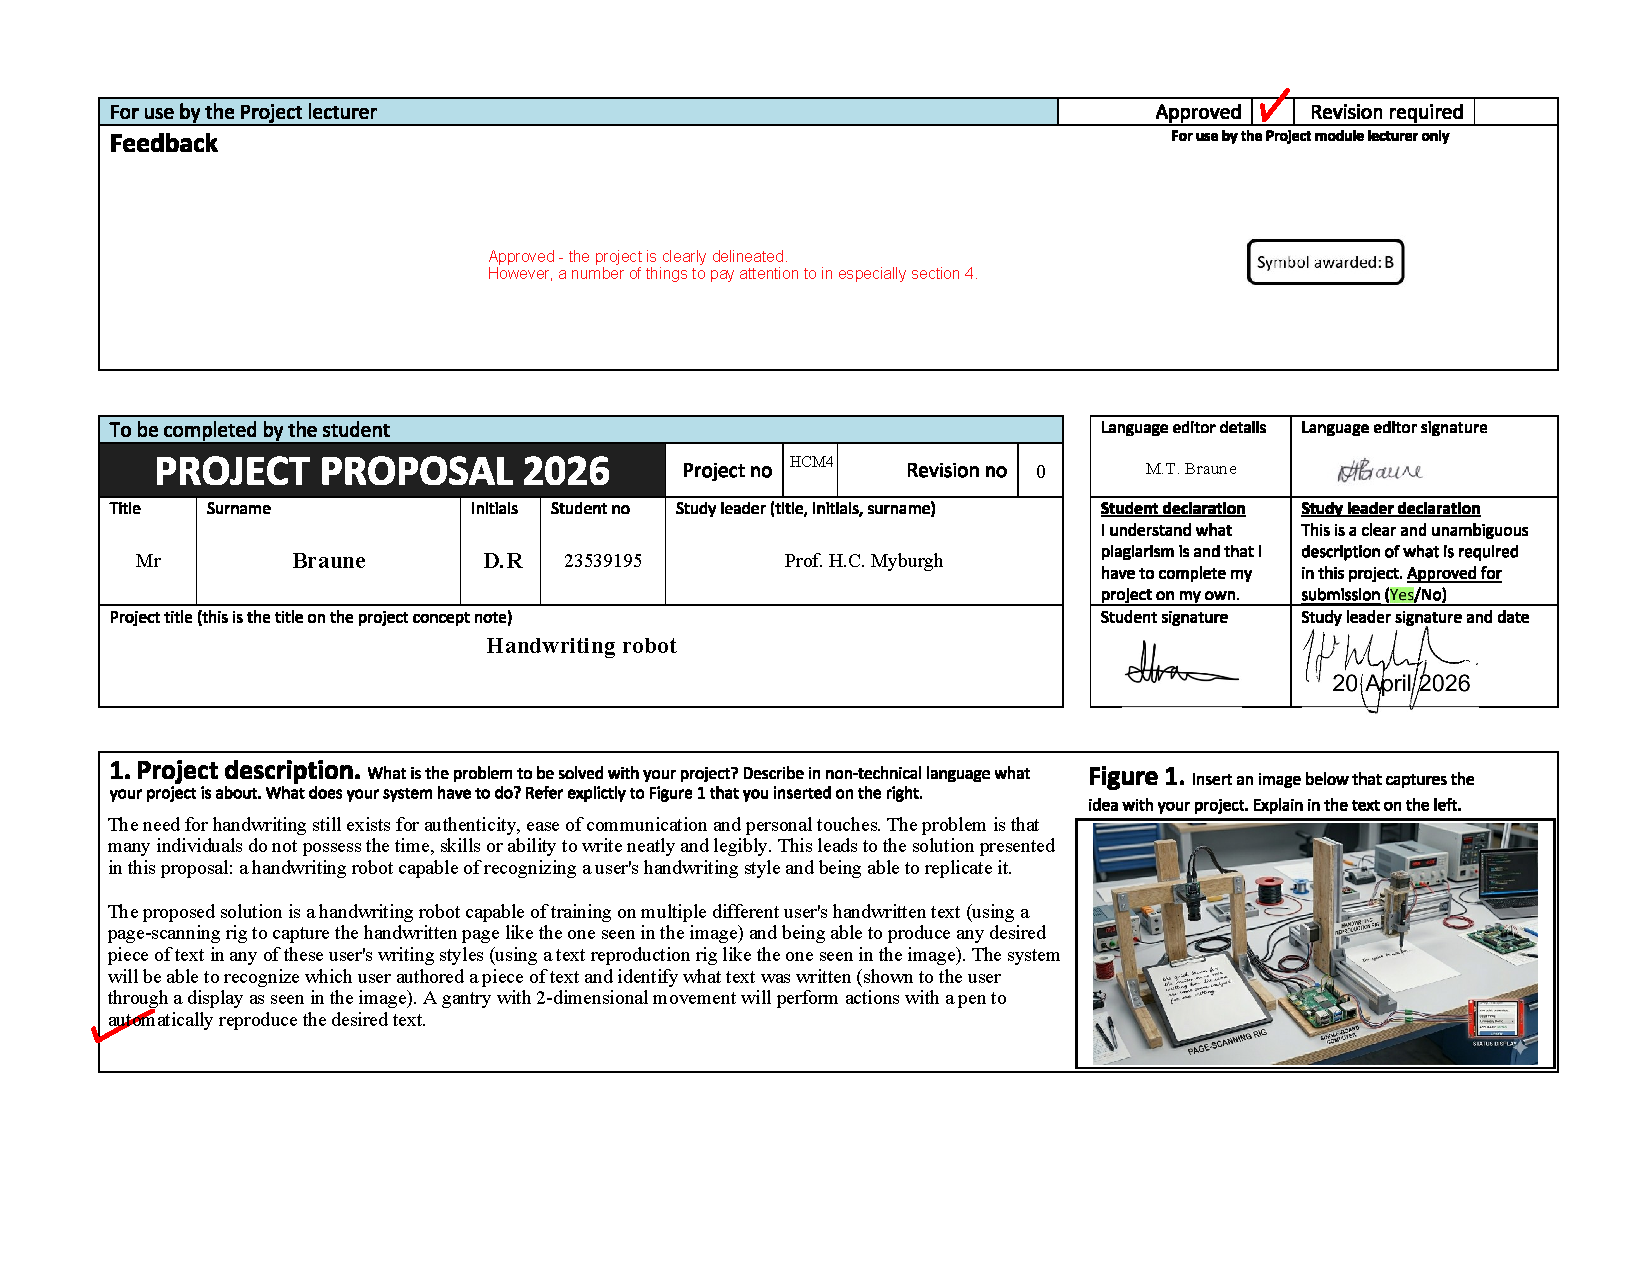
\includepdf[pages=-,landscape]{2_Project_Definition/project_proposal.pdf}

\eprsec{Part 3. Main Report}
\newpage
\pagenumbering{arabic}
\setcounter{page}{1}

\renewcommand{\eprthepartname}{Design and implementation}
\section{Literature study}
\renewcommand{\eprthepartname}{Literature study}
\label{sec:literature}
\tikzset{
  litbox/.style={draw,rounded corners=2pt,fill=gray!12,align=center,font=\footnotesize,minimum height=7mm,inner sep=3pt},
  litio/.style={draw,rounded corners=6pt,fill=white,align=center,font=\footnotesize,minimum height=7mm,inner sep=3pt},
  litarr/.style={-{Stealth[length=2.0mm]},thick},
  litlab/.style={font=\scriptsize,inner sep=1.5pt,align=center}
}
\subsection{Handwriting recognition and writer identification}
\label{sec:lit-background}
\label{sec:lit-hwr}
\subsubsection{Offline recognition and available datasets}
The ability of a computer or system to identify written text after being trained on large amounts of data is known as HWR (Handwriting Recognition) or HTR (Handwritten Text Recognition)~\cite[p.~39]{chen2023}. One type of handwritten text recognition is offline recognition, which means the data being identified by the system is static and captured post-completion of the page of handwritten text. This is ideal for identifying the text from a fixed image of handwritten content by utilising image processing techniques and algorithms to identify the text that was written~\cite[p.~268]{ma2023}. The other type is online recognition, which is a more dynamic process that uses information recorded during the creation of the handwriting. The addition of a time variable includes data about the order of strokes as well as pen-up or pen-down movements~\cite[p.~18]{graves2013}.

This project uses offline recognition because its inputs are photographed or scanned pages. The text and writer must therefore be identified from visible ink geometry. The absence of recorded stroke order also influences how the handwriting can later be reproduced: a path recovered from an image is a geometric estimate, rather than a recording of the writer's movements.

Multiple datasets have been used for training handwritten text recognition modules. The EMNIST (Extended MNIST) By\_Class dataset consists of 814\,255 handwritten characters and numbers, each being 28 by 28 pixels in size~\cite[p.~40]{chen2023}. There is only a single character per image, which suits isolated-character classification but does not itself supply examples of connected handwritten words. The IAM handwriting dataset provides complete handwritten English pages, lines and words with their transcriptions and writer metadata~\cite{marti2002}. Hemanth et al. report the expanded database as 5\,685 labelled sentences and 115\,320 labelled words from 657 writers~\cite[p.~2460]{hemanth2022}.

The dataset influences which variations the classifier encounters and which labels are available. For this project, line images and their transcripts support recognition without manually labelling every character boundary. Writer-labelled pages also support author classification and extraction of individual style profiles. IAM supplies public handwriting variation, while the personal dataset represents the project's photographed input conditions. A small isolated-character dataset alone would not address both requirements.

\subsubsection{Image conditioning and text separation}
The image conditioning of handwriting pages includes techniques performed on the handwritten text before it is passed into the classification and feature-recognition algorithms. This accounts for dimensional adjustments, removal of inconsistencies and normalisation of the data, to make the images more appropriate for text separation and classification~\cite[pp.~2458--2460]{hemanth2022}. Normalisation reduces the influence of unwanted variation; examples include min--max scaling and z-score normalisation~\cite[pp.~40--41]{chen2023}.

Binarisation differentiates the background page from the ink of the written text, computed by pixel. A global threshold taken from the grey-level histogram uses one decision level for the image~\cite{otsu1979}. A local threshold instead uses statistics from a window around each pixel and can accommodate uneven illumination~\cite[pp.~2--3]{bradley2007}. Deskewing corrects page rotation, while deslanting corrects the lean of individual characters by applying a horizontal shear. These are different transformations: aligning text lines does not require removing the writer's characteristic slant~\cite{postl1986,vinciarelli2001}.

For the camera input in this project, illumination correction and deskewing are needed before the ink is separated into lines. Slant must remain available as a writer-specific measurement; it can be removed for glyph storage and reapplied when the text is synthesised. The purpose is to suppress capture variation while retaining the information needed for reproduction.

Text separation is the process of breaking up a page of handwritten text into smaller segments or blocks that can be used in feature extraction and neural-network classifiers. Existing methods separate text into lines, words or individual characters. Hemanth et al. obtain lines and words through filtering, dilation and bounding boxes~\cite[pp.~2459--2460]{hemanth2022}. When lines are mostly straight and separated by blank rows, boundaries can be found from minima in the row ink profile. Where ascenders and descenders overlap, a boundary that bends between lines is more suitable. Minimum-cost seam methods provide a way to trace such curved boundaries~\cite[p.~3]{avidan2007}.

The project therefore separates whole lines before recognition. This avoids requiring a reliable cut between every pair of connected letters. Character boundaries are still needed to construct a glyph library, but there the known transcript and a trained line reader can constrain the extraction. Line segmentation and glyph extraction consequently solve different problems, even though both divide an image.

\subsubsection{Neural networks and feature extraction}
Many different types of neural-network models have been implemented for handwriting recognition, including artificial neural networks (ANNs), convolutional neural networks (CNNs), recurrent neural networks (RNNs) and combinations of them. ANNs consist of interconnected neurons, weights, hidden layers and biases that learn a mapping from the input to an output. CNNs use local connections and shared kernels to extract spatial patterns with fewer independent parameters than an otherwise comparable fully connected image layer~\cite[pp.~6--8]{lecun1998}. RNNs maintain a state across a sequence, allowing a prediction to depend on neighbouring evidence~\cite[p.~269]{ma2023}.

The convolutional layers of a CNN perform feature extraction by sliding a convolutional kernel over the image. Each local input value is multiplied by a corresponding kernel value, the products are summed, and a bias and activation function produce an output feature value. Reusing the kernel allows the same pattern to be detected at different locations~\cite[p.~6]{lecun1998}. For unit stride and no padding, an $N$ by $N$ input with an $f$ by $f$ kernel returns an $(N-f+1)$ by $(N-f+1)$ feature map. Pooling then reduces spatial resolution and retains selected responses~\cite[pp.~6--7]{lecun1998}. Figure~\ref{fig:lit-conv} illustrates these operations.

\begin{figure}[!htbp]
\centering
\begin{tikzpicture}[x=1cm,y=1cm,font=\footnotesize]

\draw[step=0.26,gray!50,thin] (0,0) grid (1.56,1.56);
\draw[thick] (0,0) rectangle (1.56,1.56);
\fill[gray!40,opacity=0.75] (0.26,0.78) rectangle (1.04,1.56);
\draw[very thick] (0.26,0.78) rectangle (1.04,1.56);
\node[litlab,below] at (0.78,-0.10) {input, $N\times N$};
\node[litlab,above] at (0.78,1.62) {$f\times f$ kernel slides};

\draw[litarr] (1.75,0.78) -- (2.60,0.78);
\node[litlab,above] at (2.17,0.86) {multiply,};
\node[litlab,below] at (2.17,0.72) {add bias};

\draw[step=0.26,gray!50,thin] (2.80,0.26) grid (3.84,1.30);
\draw[thick] (2.80,0.26) rectangle (3.84,1.30);
\fill[gray!40,opacity=0.75] (2.80,1.04) rectangle (3.06,1.30);
\node[litlab,below] at (3.32,0.03) {feature map,};
\node[litlab,below] at (3.32,-0.22) {$(N-f+1)\times(N-f+1)$};
\node[litlab,above] at (3.32,1.49) {activation applied};

\draw[litarr] (4.03,0.78) -- (4.88,0.78);
\node[litlab,above] at (4.45,0.86) {max-pool};
\node[litlab,below] at (4.45,0.72) {$2\times2$};

\draw[step=0.26,gray!50,thin] (5.08,0.52) grid (5.60,1.04);
\draw[thick] (5.08,0.52) rectangle (5.60,1.04);
\node[litlab,below] at (5.34,0.29) {downsampled};
\node[litlab,below] at (5.34,0.04) {feature map};

\draw[litarr,dashed] (5.79,0.78) -- (6.55,0.78);
\node[litlab,right,align=left] at (6.60,0.78) {repeated, each stage\\ holding more feature\\ maps than the last};
\end{tikzpicture}
\caption{One convolutional layer and one max-pooling layer. The kernel slides over every position of the input, so an $N\times N$ input gives an $(N-f+1)\times(N-f+1)$ feature map, which pooling then downsamples~\cite[pp.~6--8]{lecun1998}. This size expression assumes unit stride and no padding.}
\label{fig:lit-conv}
\end{figure}


The LeNet-5 model is an established example of this structure. It uses a $32\times32$ input and seven trainable layers, including convolution, subsampling and fully connected stages; its original output uses radial-basis units~\cite[pp.~7--8]{lecun1998}. A deeper alternative is a residual network, whose skip connections provide additional routes for information and gradients through the network~\cite[p.~270]{ma2023}. These examples show the choice between compact feature extraction and a more complex model; increasing depth does not guarantee an improvement for every dataset or processor.

A combination of CNNs and recurrent layers allows an entire line to be read without word or character separation. The convolutional layers convert the cropped line into feature columns, and a bidirectional recurrent layer reads the sequence in both directions, providing context from before and after each position~\cite[pp.~4--5]{kizilirmak2023}. In this offline setting, the sequence axis is the horizontal position in the image, rather than the measured time at which a pen moved. The full line crop is available before classification. Related convolutional--recurrent recognition systems use the same distinction between image features and sequence prediction~\cite[pp.~2--3]{shi2017}.

Long sequences make simple recurrent networks difficult to train because gradients can diminish or grow through repeated updates. Long short-term memory (LSTM) uses an additive memory state and gates to control what is retained, replaced and exposed~\cite[pp.~4--5]{graves2013}. The convolutional feature columns usually outnumber the transcript characters, so their alignment is initially unknown. Connectionist temporal classification (CTC) adds a blank symbol and sums the probabilities of the paths consistent with the transcript. Repeated adjacent symbols are collapsed before blanks are removed~\cite[pp.~2--4]{graves2006}. Figure~\ref{fig:lit-line} shows the resulting recognition path.

\begin{figure}[!htbp]
\centering
\begin{tikzpicture}[x=1cm,y=1cm,font=\footnotesize,node distance=4.5mm]
\node[litio,text width=1.5cm] (img) {line image};
\node[litbox,right=of img,text width=1.7cm] (cnn) {convolutional\\layers};
\node[litbox,right=of cnn,text width=1.6cm] (cols) {$T$ feature\\columns};
\node[litbox,right=of cols,text width=1.9cm] (rnn) {recurrent layer,\\both directions};
\node[litbox,right=of rnn,text width=1.6cm] (pc) {symbol per\\column};
\node[litio,right=of pc,text width=1.1cm] (out) {\texttt{the}};
\foreach \a/\b in {img/cnn,cnn/cols,cols/rnn,rnn/pc,pc/out}{\draw[litarr] (\a) -- (\b);}

\draw[litarr] ([yshift=3.2mm]rnn.north west) -- ([yshift=3.2mm]rnn.north east);
\draw[litarr] ([yshift=6.0mm]rnn.north east) -- ([yshift=6.0mm]rnn.north west);

\node[litlab,below=2.0mm of pc,font=\ttfamily\scriptsize] (sym) {-tt-h-ee};
\node[litlab,below=1.6mm of sym] {collapse repeats,\\drop the blanks};
\node[litlab,below=2.0mm of cols,text width=2.5cm] {$T$ far exceeds the\\number of characters,\\so the alignment is\\not known};
\end{tikzpicture}
\caption{Reading a whole text line without cutting out characters, after the arrangement of Kizilirmak and Yanikoglu~\cite[pp.~4--5]{kizilirmak2023}. The convolutional layers produce $T$ feature columns, a recurrent layer reads them in both directions, and a symbol including a blank is emitted per column; collapsing repeats and removing the blanks gives the transcription.}
\label{fig:lit-line}
\end{figure}


This combination is used for the project's reader because the training labels describe complete lines. The CNN extracts stroke patterns, the bidirectional LSTM retains their horizontal context, and CTC trains the network without supplied character positions. For author identification, the same convolutional architecture is useful, but its features must describe the writer across a line rather than decode an ordered transcript. The two tasks therefore require different output heads and separately trained weights.

\subsubsection{Training and assessment}
The way networks are trained corresponds to the architecture they are built from. Batch normalisation subtracts the batch mean and divides by the standard deviation, with a stabilising constant and learned scale and offset~\cite[p.~4]{ioffe2015}. Dropout reduces overfitting by removing a random subset of a layer's outputs during training, limiting dependence on individual features~\cite[pp.~1931, 1934]{srivastava2014}. Data augmentation introduces small rotations, shears or smooth distortions while retaining the transcription~\cite{wigington2017}. These methods address different sources of variation and do not replace separate validation data.

Recognition is commonly assessed through character error rate (CER) or word error rate (WER), using insertions, deletions and substitutions relative to a reference transcript~\cite[p.~2]{graves2006}. An error in one character can spoil a whole word, but word edit error is not simply a count of words at matching positions. The metric and its reference population must remain explicit when comparing systems.

For this project, numerical forward passes, backward passes and optimiser updates make the learning calculations inspectable. A corresponding library implementation supports training and comparison, with stored arrays used for NumPy inference on the ODROID. The report distinguishes the selected library-trained weights from the independently trained numerical models. Character edits, writer decisions and physical drawing measurements are evaluated separately because they measure different functions.

\subsubsection{Techniques for writer identification}
There are multiple approaches to identifying the author of a written piece of text. One uses measured, text-independent features such as slant, height, stroke width, spacing and connectivity. Another describes the distribution of edge directions and recurring letter fragments, giving a texture and shape description of the writing~\cite[p.~701]{bulacu2007}. Alternatively, a neural network learns discriminative features from examples labelled by writer~\cite{he2020}. Such a classifier identifies a writer among its trained classes; it does not automatically identify an unfamiliar person.

This project needs an author classifier to select and assess the stored writer styles, while explicit geometry measurements are needed to reconstruct their appearance. Ink-trace width can itself contain writer information~\cite[p.~162]{brink2012}, but the gantry uses its own pen. Stroke normalisation is therefore applied to reduce reliance on that cue and direct the classifier towards shape. Writer identity and stylistic fidelity remain separate measures: recognising an author does not establish that every letter or spacing feature has been reproduced accurately.

\subsection{Handwriting synthesis in a writer's style}
\label{sec:lit-synth}
Before handwritten text can be reproduced through hardware, the desired text must be created in the selected author's style. Four approaches illustrate the trade-offs between source data, learned variation and the form of the output.

\textbf{Recurrent stroke-level synthesis.} A recurrent neural network predicts the next pen movement through small coordinate offsets and an end-of-stroke indicator. It models a distribution of possible movements because no letter is written identically every time~\cite[pp.~18--20]{graves2013}. Its output is naturally suited to a plotter, but training uses online recordings. This project's offline pages contain no measured stroke order, so this approach would require a different source dataset and an additional generative model.

\textbf{Adversarial image synthesis.} A generative adversarial network trains a generator and discriminator together: one generates handwriting, while the other helps distinguish generated samples from real examples. GANwriting also constrains content and writer style to produce text images~\cite[pp.~3--7]{kang2020}. Once trained, the generator produces an image in a forward pass. This is a relevant alternative for learning contextual letterforms, but a raster output still needs conversion into the pen paths required by this project.

\textbf{Diffusion-based synthesis.} This method learns to reverse a noise-corruption process and generates handwriting through successive denoising steps. One-DM uses one reference style image at generation time, while its training uses a much larger handwriting corpus~\cite[pp.~3--5, 9]{dai2024}. A small reference requirement must therefore be distinguished from the data and computation required to train the model. For this project, diffusion would add both a separate training task and image-to-path recovery, rather than directly supplying the motion representation.

\textbf{Glyph-library synthesis.} This method assembles words from shapes or glyphs extracted from existing handwritten pages. Haines et al. store labelled forms and select and join them using information about their shape, context and spacing~\cite[pp.~4--8]{haines2016}. Their standard data collection uses approximately four A4 pages per writer~\cite[p.~4]{haines2016}. This suits the project's small personal collections and allows explicit control of size, slant and spacing. The main limitation is that a finite collection of character shapes and joining rules only approximates the way connected handwriting changes with its neighbours.

Generated handwriting can be assessed through geometric comparisons, recognition and human judgement. Haines et al. include human evaluation, while image-generation work also uses text and writer recognition to assess the output~\cite[pp.~12--14]{haines2016},~\cite[pp.~8--9]{kang2020}. For the present robot, model scores help choose a candidate before drawing, but final physical output also needs its own read-back and geometric assessment. A classifier used to select the candidate is not an independent human judgement of its style.

\subsection{Physical reproduction and pen-path mapping}
There are three relevant families of mechanism for reproducing text on paper: Cartesian systems, serial-chain robots and parallel-chain robots. A Cartesian system consists of a gantry with independent $x$--$y$ movement. Serial-chain robots consist of linkages connected in a chain, like a typical robot arm. Parallel mechanisms use several linked chains to support the moving platform~\cite[pp.~5--8]{teikari2016}. These arrangements differ in their workspace, mechanical structure and coordinate transformations.

A Cartesian gantry is suitable here because the page is flat and the main motion requirement is two-dimensional. Each axis can be commanded and calibrated separately, with a further pen-lift mechanism for travel. This makes the conversion from an image-derived path to physical coordinates direct, while leaving frame alignment, transmission compliance and missed steps as practical accuracy concerns.

A pen path is stored as a list of points, and a recovered stroke usually has more points than a plotter needs. Polyline simplification reduces this list while retaining the stroke's shape. The Douglas--Peucker method joins the endpoints, finds the point furthest from that line and retains it when its distance exceeds a chosen tolerance, then repeats on the resulting parts~\cite{douglas1973}. A small tolerance follows the stroke closely; a large tolerance removes more points but can cut corners. When handwriting exists only as an image, the path must first be recovered, for example by thinning the ink to a centreline~\cite[p.~237]{zhang1984}.

These operations are needed to turn the project's stored glyphs into manageable G-code trajectories. Simplification controls geometric detail, while the thinning and tracing determine which strokes are available to the synthesiser. Neither recovers the original writing speed or pressure from a photograph, so the controller must define its own drawing feed and pen transitions.

There are multiple methods of linear actuation that could be considered for a Cartesian plotting system, including belt drives, rack-and-pinion drives and screw drives~\cite{iqs2024}. The project uses timing belts and pulleys to convert motor rotation into movement along supported rails. This choice prioritises a straightforward, affordable page-sized mechanism with sufficient travel speed; its nominal step resolution must still be distinguished from measured positioning accuracy.

\subsection{Application of the literature}
\label{sec:lit-application}
\label{sec:lit-embedded}
The literature supports a system built around offline pages, complete-line recognition and explicit glyph geometry. Image conditioning and curved line separation prepare photographed input; convolutional features support separate text and writer outputs; transcript-guided extraction turns observed handwriting into reusable paths. A glyph library then supplies controllable geometry without training an additional handwriting generator. The Cartesian gantry provides the physical output stage. Section~\ref{sec:approach} explains how these choices were combined and developed, while Section~\ref{sec:design} gives their calculations, implementation and verification.

\clearpage
\section{Approach}
\renewcommand{\eprthepartname}{Approach}
\label{sec:approach}
The project was approached as two interacting systems: one interprets photographed handwriting and constructs writer-specific paths, while the other converts those paths into physical pen movement. The proposal's functional analysis provides their responsibilities; the G-code interface allows their implementation and verification to proceed separately.

\subsection{From functional analysis to concept}
\label{sec:app-concept}
The first concept retained page acquisition (FU~1), processing on the single-board computer (FU~2), the gantry (FU~3) and the power supply (FU~4). The final arrangement is shown in Figures~\ref{fig:des-hardware-system} and~\ref{fig:des-processing-system}. A restrained page and fixed camera supply the image. Conditioning and line segmentation prepare it for two outputs: a transcript from the sequence reader and a writer identity from the author classifier. Known transcripts separately support glyph and style extraction, producing persistent profiles from which new text can be synthesised.

The proposal's character-separation concept was developed into line-level recognition because joined handwriting does not supply a reliable boundary between every letter. Character boundaries are recovered during profile construction, where the known text constrains the problem. The writer network uses the same convolutional architecture as the reader with a different head and separate weights. Its input is stroke-normalised so the robot's pen appearance has less influence on writer identification.

The chosen physical concept is a belt-driven Cartesian gantry with two stepper motors and a separate pen-lift mechanism. The Y-axis motor drives both side belts through a cross-shaft. The ODROID coordinates the axes, monitors the switches and operates the pen motor through a transistor. This keeps planar movement directly related to the requested coordinates, while calibration establishes the usable travel and step scale.

\subsection{Development and verification sequence}
\label{sec:app-order}
The motion and processing subsystems meet at a file of G-code. This interface allows geometric commands to exercise the gantry independently of recognition and synthesis, and allows generated trajectories to be inspected before physical execution. Mechanical assembly, belt alignment, the pen mechanism and homing could therefore be developed and checked without requiring a trained handwriting model.

The processing design is presented in dependency order: page conditioning and line separation; text and writer classification; then glyph extraction, layout and trajectory generation. The line reader is needed for transcript-guided glyph alignment, and the resulting stored geometry is needed before synthesis can assemble new text. Intermediate images, numerical layer checks and independently parsed G-code provide checks at these interfaces. Formal qualification is then organised by the proposal's six requirements in Section~\ref{sec:results}.

The implementation includes a NumPy training and inference route and a corresponding library training route. Off-device training supplies the selected library-trained joint reader and eleven-writer model, while inference and motion control run on the ODROID. The numerical models are evaluated alongside the selected models. This preserves the first-principles implementation work while stating the actual training arrangement explicitly, rather than treating model preparation and embedded operation as the same task.

\subsection{Design alternatives and trade-offs}
\label{sec:app-alternatives}
The alternatives were judged against recognition and reproduction quality, processing time, available writer data, inspectability and mechanical simplicity. Table~\ref{tab:app-tradeoffs} summarises the decisions that explain the order and content of the Design section.

\begin{table}[!htbp]\centering\small
\begin{tabularx}{\linewidth}{@{}p{0.20\linewidth}XX@{}}
\toprule
\textbf{Decision} & \textbf{Alternative and trade-off} & \textbf{Selected approach and reason}\\
\midrule
Motion mechanism & Articulated or parallel robots offer different workspaces and motion, with more involved coordinate transformations~\cite[pp.~5--8]{teikari2016}. & Cartesian axes suit a flat page and allow direct coordinate commands and separate axis calibration.\\[3pt]
Recognition unit & Isolated-character classification is simpler but depends on character cuts; a sequence reader needs a larger model. & Whole-line CNN--BiLSTM--CTC recognition uses the available transcripts and handles connected text without pre-cut letters~\cite[pp.~4--5]{kizilirmak2023}.\\[3pt]
Writer representation & Photographed ink retains pen-width cues; normalisation removes some information as well as nuisance variation. & Stroke-normalised classification emphasises geometry that can be reproduced with the gantry's own pen.\\[3pt]
Synthesis method & Neural stroke generators need online data; learned image generators need training and subsequent path recovery~\cite[p.~18]{graves2013},~\cite[p.~9]{dai2024}. & A glyph library uses the available offline pages and exposes controllable trajectories, at the cost of weaker contextual joining~\cite[p.~4]{haines2016}.\\[3pt]
Implementation & A framework provides practical training; explicit numerical operations expose layer calculations but have substantial training cost. & Both routes are retained. Selected weights are exported to arrays for NumPy inference, with numerical checks and trained-model comparisons reported separately.\\
\bottomrule
\end{tabularx}
\caption{Principal concept choices and their engineering trade-offs.}
\label{tab:app-tradeoffs}
\end{table}

The design also considers page loading, preview before movement, switch feedback, motor-power distribution, component reuse and contributor consent. These considerations shape the interfaces and construction; their practical consequences are evaluated in Discussion. Design consequently begins with the hardware and its constraints, then follows segmentation, classification, reproduction and integration. Detailed equations belong there, rather than in this conceptual overview.

\clearpage
\renewcommand{\eprthepartname}{Design and implementation}
\section{Design and implementation}
\label{sec:design}
The Cartesian plotter constrains the workspace, pen state and motion required from the software. The design therefore starts with hardware, then follows page segmentation, text/writer classification and handwriting reproduction, before describing their integration.

Numerical substitutions use the configured mechanism and recorded processing of stored handwriting, with inputs and scope collected in Appendix~\ref{app:des-real-calculations}. Borrowed methods are referenced where introduced; project-specific transforms and heuristics are identified as design choices. These traces show how the calculations operate; physical qualification remains in Results.\par

\subsection{Design summary}
\label{sec:des-summary}
This section summarises the project design tasks and how they were implemented (see Table~\ref{tab:des-summary}). The tasks follow the deliverables and student design work in the approved Project Proposal. Completion refers to the implementation of a task; compliance with a numerical system specification is established separately by the qualification tests in the Results section.

\begin{table}[!htbp]
\centering\small
\begin{tabularx}{\linewidth}{|>{\raggedright\arraybackslash}p{0.24\linewidth}|>{\raggedright\arraybackslash}X|>{\raggedright\arraybackslash}p{0.23\linewidth}|}
\hline
\textbf{Deliverable or task}&\textbf{Implementation}&\textbf{Completion and report location}\\\hline
Investigation of methods&Compared recognition, conditioning and reproduction approaches.&Completed; Literature Review; Sections~\ref{sec:des-class}, \ref{sec:des-reproduction}.\\\hline
Page capture and image conditioning&Camera arrangement, illumination normalisation, ink extraction and orientation correction.&Completed; Sections~\ref{sec:des-camera} and~\ref{sec:des-seg}.\\\hline
Separation of handwritten text&Line detection, curved boundaries and ink ownership; later transcript-constrained glyph localisation.&Completed; Sections~\ref{sec:des-seg}, \ref{sec:des-alignment}.\\\hline
Text and writer classifiers&Convolutional features, sequence recognition and writer identification.&Completed; Section~\ref{sec:des-class}.\\\hline
Network training implementations&NumPy calculations and framework training; selected weights are framework-trained.&Completed; Sections~\ref{sec:des-training}--\ref{sec:des-netverify}.\\\hline
Writer-specific trajectory maps and storage&Aligned glyph extraction, skeleton tracing, variant filtering and persistent style profiles.&Completed; Sections~\ref{sec:des-alignment}--\ref{sec:des-profile}.\\\hline
Handwriting synthesis and G-code&Text layout, glyph assembly, candidate selection and conversion to machine coordinates.&Completed; Sections~\ref{sec:des-layout}--\ref{sec:des-gcode}.\\\hline
Gantry, pen mechanism and motion control&Custom mechanical assembly, two-axis drive, pen switching, end stops and calibration.&Completed; Section~\ref{sec:des-hardware}.\\\hline
Processing and motion integration&Server connects capture, processing, stored profiles and execution.&Completed; Section~\ref{sec:des-integration}.\\\hline
Subsystem verification&Numerical checks and offline image/path experiments; formal integrated qualification is reported in Results.&Completed; Sections~\ref{sec:des-netverify}, \ref{sec:des-segverify}; Appendix~\ref{app:des-visual-tests}.\\\hline
\end{tabularx}
\caption{Design summary.}
\label{tab:des-summary}
\end{table}

\FloatBarrier

\subsection{System block diagram}
\label{sec:des-system}
Figure~\ref{fig:des-hardware-system} shows the hardware connections for page capture, handwriting interpretation and physical reproduction. Figure~\ref{fig:des-processing-system} shows the corresponding software paths. The explanations follow each diagram's numbered groups.

\begin{figure}[!ht]\centering
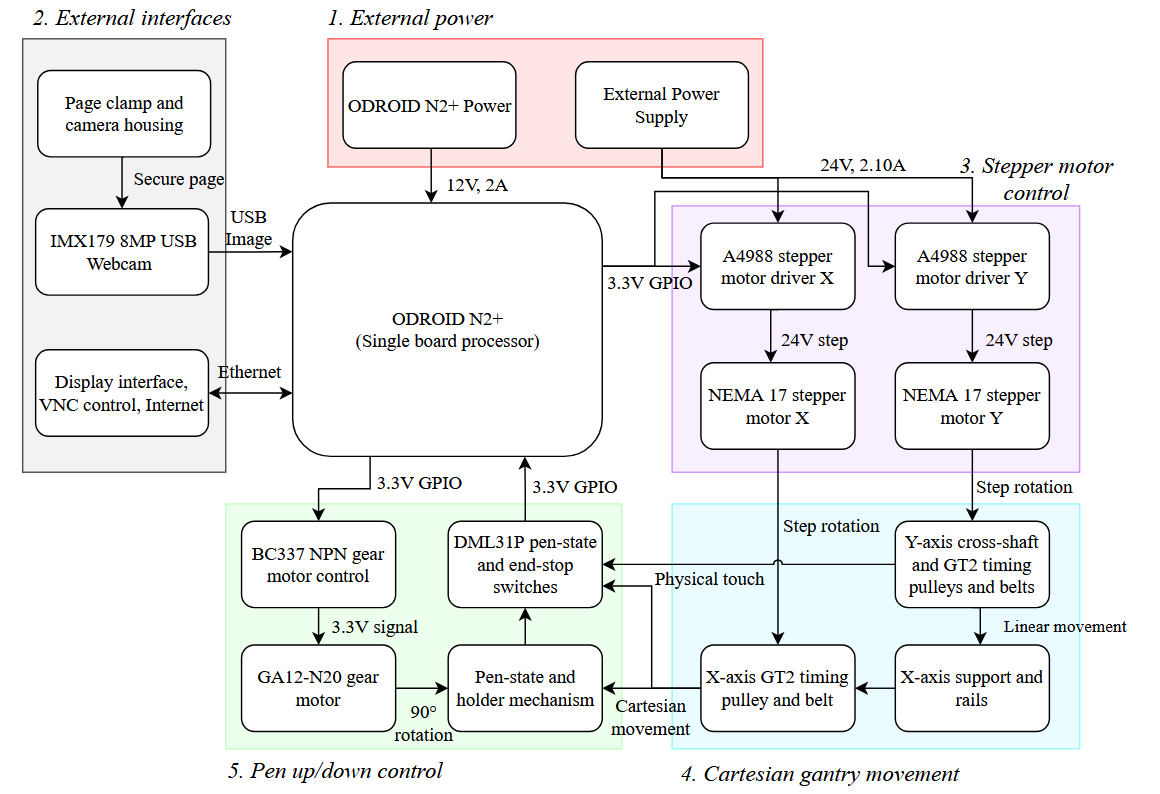
\includegraphics[width=0.96\linewidth]{Evidence/user_hardware_diagram_input.png}
\caption{Hardware system block diagram supplied by the author. The detailed controller pins, signal levels and power connections are listed in Table~\ref{tab:des-pin-map}.}
\label{fig:des-hardware-system}
\end{figure}
\FloatBarrier

\noindent\textbf{1. External power.} Separate supplies power the ODROID and the 24~V motor rail. The ODROID's dedicated 3.3~V supply pin powers the driver logic and pen motor; its GPIO pins provide control signals.

\noindent\textbf{2. External interfaces.} The page clamp holds the handwriting beneath the IMX179 USB camera, which sends images to the ODROID. The network provides interface access and remote control.

\noindent\textbf{3. Stepper motor control.} The ODROID sends STEP and DIR signals to the two A4988 drivers. Each driver regulates winding current from the 24~V rail to rotate its NEMA~17 axis motor.

\noindent\textbf{4. Cartesian gantry movement.} GT2 pulleys and belts convert motor rotation into linear X--Y motion along the rails. The Y-axis cross-shaft mechanically couples the two side belts to move the supported X-axis rail together.

\noindent\textbf{5. Pen up/down control.} A GPIO-controlled BC337 transistor switches the GA12-N20 gear motor to raise or lower the pen holder. Five switches return feedback to the ODROID: four indicate axis limits and one reports the raised pen state.

\clearpage
\begin{figure}[!ht]\centering
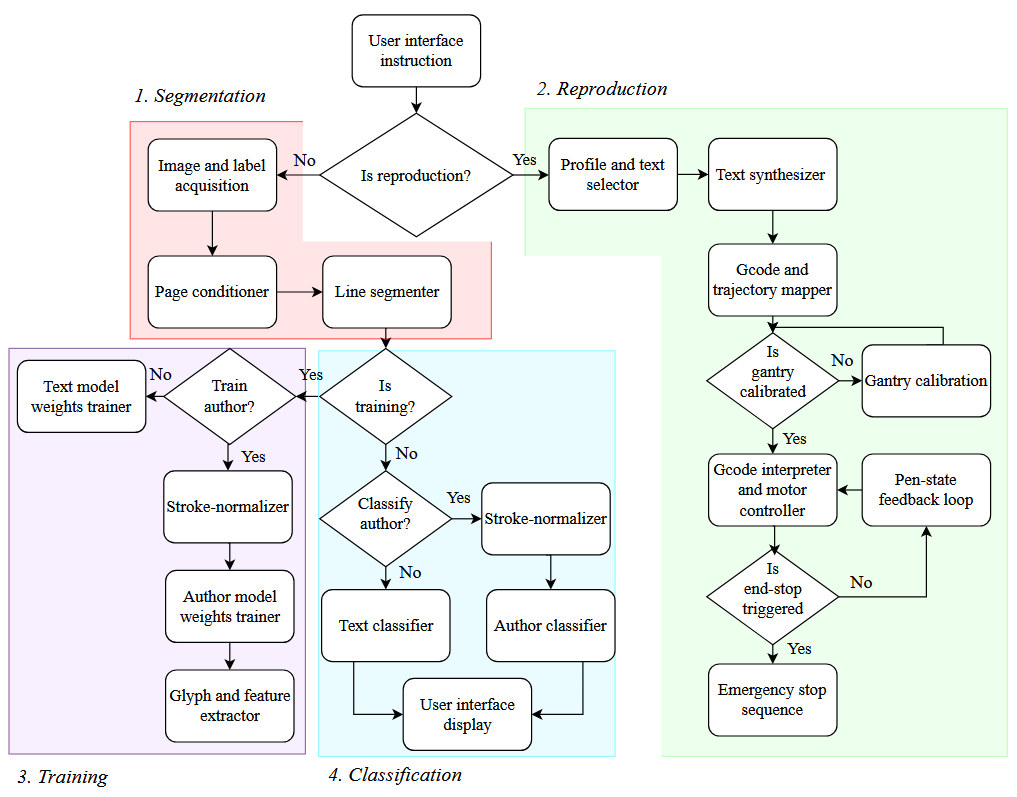
\includegraphics[width=0.98\linewidth]{Evidence/user_software_diagram_input.png}
\caption{Software system block diagram supplied by the author: (1) segmentation, (2) reproduction, (3) training and (4) classification.}
\label{fig:des-processing-system}
\end{figure}
\FloatBarrier

\noindent\textbf{1. Segmentation.} For an image-processing request, the system acquires the page and any available transcript labels. The page conditioner corrects orientation and uneven illumination, and the line segmenter separates the handwriting into line crops. These crops feed either training or classification; transcript labels are needed for supervised preparation, while classification estimates unknown content.

\noindent\textbf{2. Reproduction.} A writing request selects a stored writer profile and new text. The text synthesiser arranges the profile's glyph paths and scores candidate renderings, then the trajectory mapper converts the selected layout into G-code. Once the gantry is calibrated, the interpreter converts these commands into axis and pen-control signals. Pen-state feedback coordinates lifting and lowering, while a confirmed end-stop trip invokes the stop and recovery sequence. This is a separate request from reading a page.

\noindent\textbf{3. Training.} Segmented, labelled lines prepare the text and author models. The author route first normalises stroke thickness to the selected 0.17 x-height ratio. Transcript-guided glyph and feature extraction builds the writer profiles used for reproduction. Model training and profile extraction are separate preparation tasks: their saved weights and libraries are reused during operation. Weight training takes place off-device; page processing and motion control run on the ODROID.

\noindent\textbf{4. Classification.} The text classifier reads each complete line, while the author classifier identifies its writer after stroke normalisation. The two branches represent the requested outputs; a page report can contain both recognised text and writer identity. Line-level writer evidence is pooled before the results are returned to the interface. Character boundaries for profile construction are recovered separately using known transcripts, rather than requiring isolated letters before recognition.

The numbered groups retain the proposal's functional units: acquisition implements FU~1; conditioning and line preparation implement FU~2.1--2.2; classification implements FU~2.3; weight training implements FU~2.4; and glyph extraction, storage and retrieval implement FU~2.5--2.7. G-code conversion and interpretation implement FU~2.8, linking the software to the axis drives and pen mechanism in FU~3.1--3.4.
\FloatBarrier

\subsection{Hardware design}
\label{sec:des-hardware}
The hardware must hold the paper and pen securely, reach the required writing area, and convert a stored trajectory into repeatable motion. The design therefore combines a Cartesian belt drive with a separately actuated pen mechanism. The electrical interface is kept simple enough for direct control from the ODROID, while calibration relates software coordinates to the travel of the assembled machine.

\subsubsection{Plotter mechanics and mechanical construction}
The chosen method of text plotting is a Cartesian gantry system with two independent axes of movement and a pen up/down mechanism, consistent with the Cartesian arrangement illustrated by Teikari~\cite[p.~6]{teikari2016}. Complex kinematic equations and joint-dependent position errors are avoided by using separate $x$ and $y$ movements for reproduction. Linear GT2 timing belts and pulleys are used to convert rotary motion from stepper motors and axles to the desired Cartesian movements. Timing belts were chosen for their cost effectiveness and ability to provide relatively fast travel without a lead-screw transmission.

A Cartesian gantry consists of stationary rails that guide movement in one axis, and a movable rail that guides the other axis of movement. For this system and the explanations that follow, the stationary rails guide $y$-axis movement, while the $x$-axis rail moves along the $y$-axis. Figure~\ref{fig:des-gantry-axes} shows the axes of the gantry.

\begin{figure}[!htbp]\centering
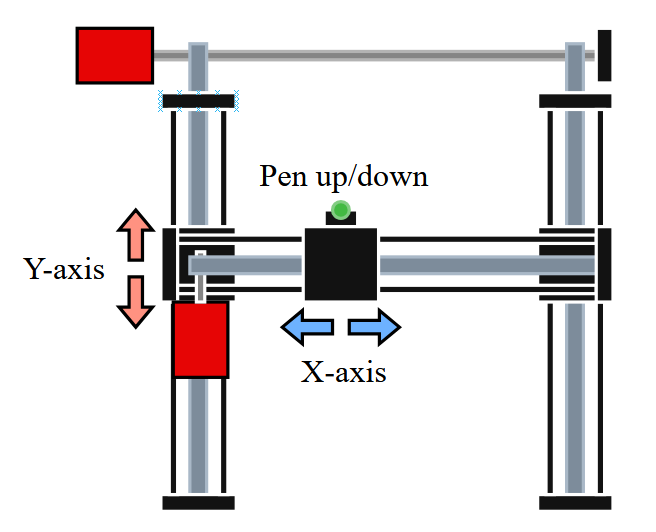
\includegraphics[width=0.67\linewidth]{Figures/gantry-axis-diagram.png}
\caption{Cartesian gantry axes and pen up/down mechanism.}
\label{fig:des-gantry-axes}
\end{figure}

The $x$-axis rail needs to move with stability and consistency, which is why it is supported at both ends by the two $y$-axis rails. A single stepper motor was chosen to drive the pulleys on both sides to ensure synchronised motion and save costs. Two independent stepper motors driving one axis introduce a synchronisation concern because differences in missed steps or loading could offset one side relative to the other. The challenge with using one motor to drive two timing pulleys is extending its shaft to both pulleys without excessive load or twist in the new axle. A rigid coupler was used to extend the stepper motor shaft with a chromed steel rod.

To reduce strain on the motors and allow smoother movement, linear bearings were fitted around the chromed rod rails so that the moving parts slide with low resistance. Bearing alignment is important as well as bearing diameter: an incorrectly aligned bearing can constrain the same rod in a different direction from the neighbouring bearing, increasing resistance instead of reducing it. During assembly, bearing fit and printed-part alignment were checked by sliding the parts along the rods before connecting the belts. The fit was adjusted where the assembled bearings restricted movement.

The shared shaft couples the two sides mechanically, but does not remove all sources of error. Unequal belt tension, shaft torsion and a frame that is not square can still change the pen position. Belt tension must therefore be sufficient to maintain engagement without adding unnecessary bearing load. The pen holder also needs enough stiffness to prevent lateral deflection as the direction of travel changes. These effects concern physical accuracy and cannot be inferred from the nominal step resolution alone.

The printed components locate bearings, support the motors and pulleys, fasten the belts, and guide the pen mechanism. The arrangement fixes the relative positions of the rail, belt and pen, so manufacturing fit and bracket stiffness affect the same position budget as the drive. The available travel is established in Section~\ref{sec:des-calibration}.

\subsubsection{Stepper motor selection and drive resolution}
\label{sec:des-drive}
A stepper motor turns through fixed angular increments as the winding-current pattern changes. The windings are the motor's coils, and each current pattern establishes a magnetic field that pulls the rotor towards a corresponding position. The A4988 regulates these winding currents by chopping: it switches the drive to maintain the requested current level. Chopping continues even while a position is held; advancing the requested current pattern, rather than chopping itself, produces the next step~\cite[p.~9]{a4988ds}.

Two stepper motors are used in the gantry plotter, one for the $x$ and one for the $y$ direction. The selected motor is the 42BYGH40-01 NEMA 17 bipolar stepper, with a 40\,mm body length, a $1.8^\circ$ full-step angle and a rated current of 1.68\,A per phase. Stepper control suits the required position commands because displacement follows from the number of commanded steps, without requiring an encoder for normal operation. The corresponding limitation is that the controller cannot determine whether every commanded step was physically completed.

Using the stepper transmission relationship~\cite{acarnley2002}, Equation~\ref{eq:des-pulley} derives the travel per revolution and pitch radius for the installed 20-tooth GT2 pulleys and 2\,mm belt pitch. The radius is determined by tooth pitch, rather than by measuring the shaft or outside pulley diameter.

\begin{equation}
\ell_{\mathrm{rev}}=N_t p=20(2)=40\ \mathrm{mm/rev},\qquad
r_p=\frac{N_t p}{2\pi}=6.37\ \mathrm{mm}.
\label{eq:des-pulley}
\end{equation}

Here $N_t$ is the tooth count and $p$ is belt pitch. The A4988 supports a microstep subdivision of $\mu_s=16$~\cite[p.~6]{a4988ds}. Combining this with 200 full steps per revolution gives the nominal displacement in Equation~\ref{eq:des-stepres}.

\begin{equation}
\kappa_0=\frac{200\mu_s}{\ell_{\mathrm{rev}}}=80\ \mathrm{microsteps/mm},\qquad
\Delta x_0=\frac{1}{\kappa_0}=0.0125\ \mathrm{mm}.
\label{eq:des-stepres}
\end{equation}

The A4988 supports this subdivision through its microstep-selection inputs~\cite[p.~6]{a4988ds}. The value in Equation~\ref{eq:des-stepres} is substantially smaller than the proposal's 0.5\,mm positional-error limit. It establishes adequate command granularity, but is not a measurement of accuracy: belt compliance, frame geometry, switch behaviour and pen deflection remain between the step count and the mark on paper. Microstepping also does not guarantee that every intermediate mechanical position is equally accurate under load.

Motor torque must be assessed at operating speed, rather than from holding torque alone. The generated Owen job uses a travel feed of 2400\,mm/min and drawing feed of 900\,mm/min. With the installed 40\,mm/revolution transmission, these correspond to 60 and 22.5\,rev/min respectively, using Equation~\ref{eq:des-rpm}.

\begin{equation}
n=\frac{F}{\ell_{\mathrm{rev}}}=\frac{2400}{40}=60\ \mathrm{rev/min}.
\label{eq:des-rpm}
\end{equation}

The load model in Equation~\ref{eq:des-torque} combines the standard linear-force and rotary-inertia relationships for a stepper-driven load~\cite{acarnley2002}, separating translation and rotation. It applies to the belt-driven axis, with all lengths expressed in metres.

\begin{equation}
T_{\mathrm{req}}=r_p(F_f+ma)+J_{\mathrm{rot}}\frac{a}{r_p}.
\label{eq:des-torque}
\end{equation}

Here $F_f$ is the resisting linear force, $m$ is the translating mass, $a$ is linear acceleration, and $J_{\mathrm{rot}}$ is the combined inertia of rotating parts referred to the motor shaft. The second axis carries the first-axis assembly, so its load must include that assembly. The rotational term must not also be included in $m$, which would count the same inertia twice. Equation~\ref{eq:des-torque} follows from $T=r_pF$ and angular acceleration $a/r_p$; it is a load calculation, not a substitute for the motor's measured torque--speed characteristic~\cite{acarnley2002}.

At constant speed, Equation~\ref{eq:des-torque} reduces to $T=r_pF_f=0.006366F_f$\,N\,m for the installed pulley, with $F_f$ in newtons. A numerical load margin requires measured carriage resistance, moving mass and reflected inertia. The available record does not establish these quantities sufficiently to substitute a verified operating load. The driver starts each segment without a controlled acceleration ramp, so a holding-torque rating alone cannot establish an allowable starting rate.

The ODROID coordinates the two axes using an integer error accumulator. For a move of $a_x$ and $a_y$ microsteps with $a_x\geq a_y$, the $x$ axis is stepped on each iteration. The accumulator is reduced by $a_y$ and a $y$ step is inserted whenever it crosses zero, before adding $a_x$ back. This is the Bresenham interpolation principle~\cite[p.~28]{bresenham1965}; it preserves the commanded endpoint and distributes the minor-axis steps along the line instead of completing one axis first.

Algorithm~\ref{alg:des-stepping} gives the major-axis form of the implemented loop. In the generated Owen file, the segment from $(17.024,239.996)$ to $(17.065,239.643)$\,mm produces signed count changes $(3,-29)$ at the configured nominal 80 microsteps/mm. For example, the $x$ increment is $\operatorname{round}(17.065\times80)-\operatorname{round}(17.024\times80)=1365-1362=3$. The $y$ axis is therefore the major axis, with initial accumulator $\lfloor29/2\rfloor=14$; the three $x$ pulses are distributed among the 29 $y$ pulses. This evaluates the generated command at the nominal scale, rather than assuming a recovered physical homing count.

\begin{designalgorithm}
\caption{Coordinated axis stepping with interruption checks}
\label{alg:des-stepping}
\prequire{Signed axis counts; pulse delay; connected GPIO interface.}
\begin{designpseudo}
\pstate{0}{$(N_M,N_m)\leftarrow$ major and minor absolute counts; set directions}
\pstate{0}{$e\leftarrow\lfloor N_M/2\rfloor$}
\pstate{0}{\textbf{for} $i\leftarrow1$ \textbf{to} $N_M$ \textbf{do}}
\pstate{1}{\textbf{if} abort requested or end stop confirmed \textbf{then}}
\pstate{2}{\textbf{return} interrupted, current position counters}
\pstate{1}{\textbf{end if}}
\pstate{1}{Pulse major axis; update its signed counter}
\pstate{1}{$e\leftarrow e-N_m$}
\pstate{1}{\textbf{if} $e<0$ \textbf{then}}
\pstate{2}{Pulse minor axis; update its signed counter; $e\leftarrow e+N_M$}
\pstate{1}{\textbf{end if}}
\pstate{0}{\textbf{end for}}
\pstate{0}{\textbf{return} completed, current position counters}
\end{designpseudo}
\end{designalgorithm}

The geometry and timing of this loop must be considered separately. The current implementation sleeps inside each axis-pulse call, so an iteration containing two pulses takes longer than one containing a single pulse. For major- and minor-axis counts $N_M$ and $N_m$, Equation~\ref{eq:des-pulsetime} gives the delay contribution, excluding GPIO and interpreter overhead.
\begin{equation}
t_{\mathrm{delay}}=(N_M+N_m)\tau,\qquad
\tau=\max\left(\frac{d}{vN_M},2\times10^{-6}\right),\quad v=F/60.
\label{eq:des-pulsetime}
\end{equation}
For that same generated segment, $d=\sqrt{0.041^2+0.353^2}=0.355373$\,mm, $v=900/60=15$\,mm/s, $N_M=29$ and $N_m=3$. Equation~\ref{eq:des-pulsetime} gives $\tau=0.355373/(15\times29)=0.000816950$\,s and $t_{\rm delay}=32\tau=0.0261424$\,s. The geometric feed budget is $d/v=0.0236915$\,s. The extra delay follows from the separate minor-axis pulses; neither value is a measured motor execution time.

Here $d$ is move length in millimetres and $v$ is the requested speed in mm/s. Equation~\ref{eq:des-pulsetime} means that a $45^\circ$ move has approximately twice the intended delay contribution, whereas an axis-parallel move does not. A shared pulse scheduler could reduce this directional speed variation. The present arrangement maintains simple coordinated positioning, but its feed value must not be treated as a measured trajectory speed.

Figure~\ref{fig:vt-stepping} makes the integer pulse distribution visible on another segment from a generated job, with count changes $(+6,-28)$. The major axis advances at every iteration, while the accumulator distributes the six minor-axis pulses. The plotted deviation from the ideal line reaches 0.5 microsteps, equivalent to $0.5/80=0.00625$\,mm at the nominal scale. This is the quantisation of the commanded path, not the mechanical error of the pen.

\begin{figure}[!htbp]\centering
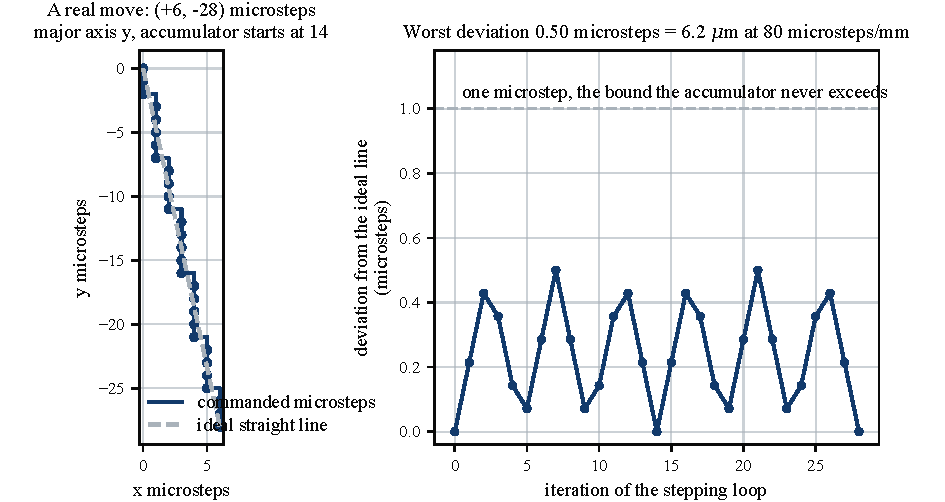
\includegraphics[width=\linewidth]{Figures/VisualTests/T52_bresenham_staircase.pdf}
\caption{Integer stepping and command-space deviation for one generated move; evaluated offline.}
\label{fig:vt-stepping}
\end{figure}

\subsubsection{Pen lift mechanism and drive circuit}
\label{sec:des-pen}
The pen has two required states: in contact with the page for a stroke, and clear of the page for travel. A compact geared motor and cam provide these states without adding a third positioning axis. The motor turns in one direction and the cam alternates the pen height as it rotates. A switch indicates the raised state. Compared with a servo, this arrangement uses a simple switched output and position indication, but it gives no commanded intermediate pen height or force.

Figure~\ref{fig:des-penmechanism} shows the two pen positions. The holder and page support are part of the same design decision: repeatable motor movement is of little value if a flexible holder changes the nib position or if a stack of paper changes contact pressure. A single restrained sheet on a rigid support reduces this variation. The mechanism was adjusted experimentally to achieve clearance during travel without excessive pressure during drawing.

\begin{figure}[!htbp]\centering
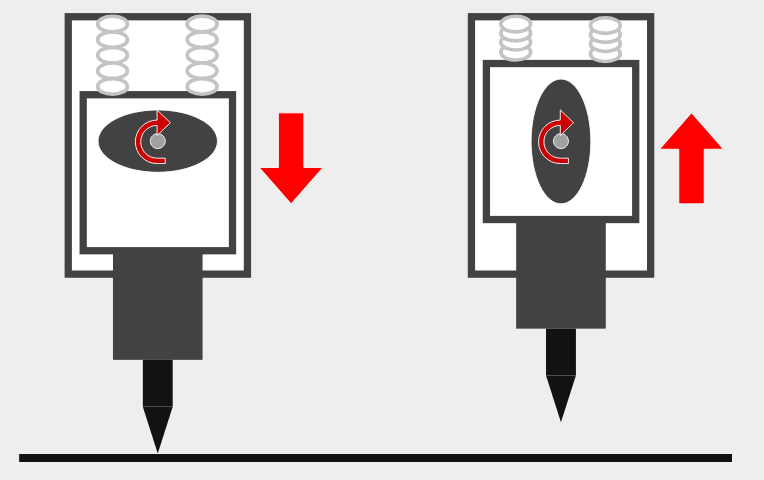
\includegraphics[width=0.66\linewidth]{Figures/pen-up-down-mechanism.png}
\caption{Cam-operated mechanism with the pen lowered and raised.}
\label{fig:des-penmechanism}
\end{figure}

The software checks the switch before energising the motor. If the desired state is already present, no pulse is required; an unnecessary rotation could move the pen away from the requested state. Otherwise the motor runs until the switch indicates the target or the timeout expires. The current control routine allows a 40\,ms overrun after confirmation of the raised state to seat the cam. This feedback operation differs from the G-code generator's settling dwell, which is described in Section~\ref{sec:des-gcode}.

The low-side BC337 circuit in Figure~\ref{fig:des-pencircuit} keeps the motor current out of the GPIO signal path. With a 1\,k$\Omega$ base resistor and the assumed $V_{BE}=0.7$\,V, Equation~\ref{eq:des-basecurrent} gives the approximate base current using the standard low-side resistor relation~\cite{rohmlowside2026}.
\begin{equation}
I_B=\frac{V_{\mathrm{GPIO}}-V_{BE}}{R_B}
=\frac{3.3-0.7}{1000}=2.6\ \mathrm{mA}.
\label{eq:des-basecurrent}
\end{equation}

The calculation in Equation~\ref{eq:des-basecurrent} establishes the nominal signal current only. It does not prove transistor saturation at motor startup or stall. The installed motor current, GPIO capability and transistor saturation conditions must be considered together~\cite{bc337ds}. Increasing base current without checking the GPIO rating would transfer the problem to the computer interface.

\begin{figure}[!htbp]\centering
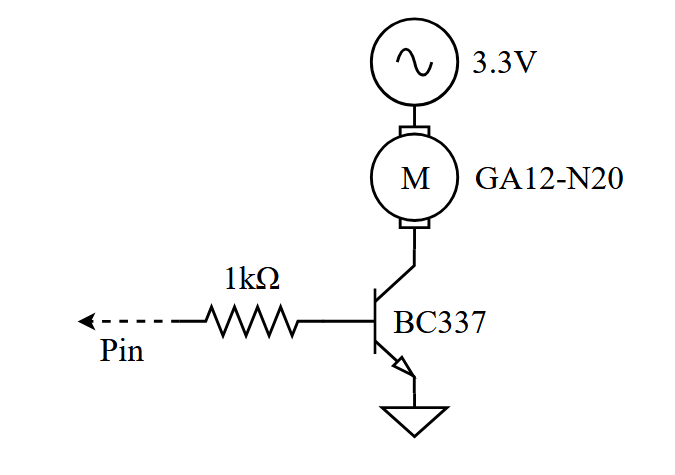
\includegraphics[width=0.60\linewidth]{Figures/pen-clicker-bc337-circuit.png}
\caption{Prototype pen-motor switching circuit. The supply arrangement and protection limitations are discussed below.}
\label{fig:des-pencircuit}
\end{figure}

The installed pen motor is powered from the ODROID's dedicated 3.3\,V supply pin, while the GPIO controls the transistor base through its resistor. The power pin and signal pin have different roles; moving the supply connection away from GPIO does not by itself establish that the rail can supply motor startup current. No flyback diode is fitted. Interrupting an inductive motor current can therefore impose a voltage transient on the switching stage~\cite{rohmlowside2026}. A diode across the motor, reverse-biased during normal operation, would provide a recirculation path; its current and voltage ratings must be selected from the motor and supply conditions. This is a limitation of the installed circuit, not a protection feature already implemented.

\subsubsection{End stops, homing and dimensional calibration}
\label{sec:des-calibration}
Four switches define the minimum and maximum travel of the two axes. Each is connected as an active-high input with a 10\,k$\Omega$ pull-down, as shown in Figure~\ref{fig:des-switch}. The pull-down defines the input while the contact is open. With the contact closed, its current is $3.3/10000=0.33$\,mA and dissipation is approximately 1.1\,mW. The resistor is between input and ground, so it does not limit fault current if the GPIO is incorrectly configured as an output driven low.

\begin{figure}[!htbp]\centering
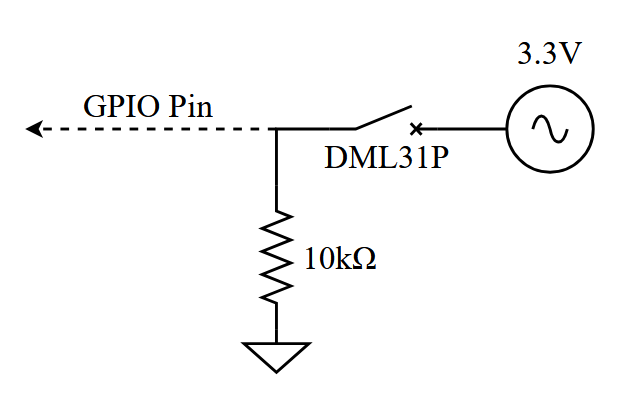
\includegraphics[width=0.62\linewidth]{Figures/endstop-switch-pulldown-circuit.png}
\caption{Active-high switch input with a 10\,k$\Omega$ pull-down.}
\label{fig:des-switch}
\end{figure}

The control routine confirms a high reading with two further samples separated by 6\,ms. Requiring three consistent readings rejects brief transients, at the cost of waiting approximately 12\,ms when a potential trip is checked. Axis pulses are not continuously generated during this blocking check, so multiplying the full confirmation interval by the commanded feed would not correctly describe the software's movement during debounce. Physical stopping distance also depends on the mechanics; it requires a measurement rather than a software-delay calculation alone.

After startup, the step counters do not establish a known physical origin. Calibration therefore drives one axis towards either switch, reverses towards the other, and counts the switch-to-switch steps. Equation~\ref{eq:des-calibration} converts this count to the scale used for motion.

\begin{equation}
\kappa_x=\frac{N_x}{L_x},\qquad \kappa_y=\frac{N_y}{L_y},\qquad
n_x=\operatorname{round}[(x+e)\kappa_x].
\label{eq:des-calibration}
\end{equation}
The configured travel dimensions give usable spans $200.6-2(5)=190.6$\,mm and $261.3-2(5)=251.3$\,mm after edge clearance. These values define the generated job's workspace. The numerical calibrated values of $\kappa_x$ and $\kappa_y$ additionally require the actual switch-to-switch counts $N_x,N_y$; a count has not been substituted where its measurement is unavailable.

Here $N_x,N_y$ are measured step counts, $L_x,L_y$ are the independently measured switch-to-switch travels, and $e=5$\,mm is the edge clearance. The corresponding expression applies to $y$. An axis retracts from the switch after calibration, and the origin lies inside the physical boundary. Absolute target counts are rounded and differenced against the tracked count, so rounding of one segment is not repeatedly accumulated as a new relative position error.

The recorded travel constants in the current code are $L_x=200.6$\,mm and $L_y=261.3$\,mm. With 5\,mm clearance on both ends, the software travel limits are 190.6 by 251.3\,mm before the writing margins are applied. These are configuration values describing the available travel; a separate calibration record is needed to state the measured microsteps per millimetre. The result of calibration is not retained as a valid position across a restart.

Calibration compensates for scale error, but it cannot correct an imprecise reference measurement. If the travel measurement has error $\delta L$, its first-order contribution to position error at commanded distance $x$ follows from the sensitivity-coefficient approach~\cite[pp.~18--19]{jcgm2008}, giving Equation~\ref{eq:des-scaleerror}.
\begin{equation}
|\delta x|\simeq |x|\frac{|\delta L|}{L}.
\label{eq:des-scaleerror}
\end{equation}

At the configured maximum $x$ travel, the multiplier in Equation~\ref{eq:des-scaleerror} is $190.6/200.6=0.95015$. Thus reference-length uncertainty contributes approximately $0.95015|\delta L_x|$ at the far end of the usable axis. This converts the actual geometry into a sensitivity coefficient; a measured uncertainty still requires the travel measurement and switch-repeatability record.

\subsubsection{Electrical integration and power distribution}
\label{sec:des-power}
The motor-driver supply is operated at 24\,V. The recorded supply-current indication is 0.35\,A, with the supply current limit set to 2.11\,A. These quantities have different meanings: the first is a reading at an operating condition, the second limits the available supply current, and neither specifies the winding-current regulation of an A4988. At the recorded operating condition, that supply delivers approximately $24(0.35)=8.4$\,W. This reading does not include a verified peak-load test or establish total consumption from both supplies.

The ODROID-N2+ header provides 3.3\,V digital I/O, and the A4988 logic supply operates from 3\,V to 5.5\,V~\cite{odroidn2ds},~\cite[p.~5]{a4988ds}. With the drivers' logic supply connected to 3.3\,V, the A4988 minimum high input is $0.7(3.3)=2.31$\,V~\cite[p.~4]{a4988ds}. A nominal 3.3\,V ODROID output therefore has $3.3-2.31=0.99$\,V of nominal high-level margin. This is a compatibility calculation from specified levels, not a measurement at the installed driver pins. Hardkernel recommends a 12\,V, 2\,A adapter for the board, but the actual adapter fitted to this system has not been identified; the value shown in the supplied sketch is therefore not treated as a measured supply specification~\cite{odroidn2ds}.

Table~\ref{tab:des-pin-map} maps each motion-controller connection to the ODROID 40-pin header. Physical header numbers and \texttt{gpiochip0} line offsets are listed separately because they are different numbering systems. The assignments follow the active controller configuration in \texttt{Software/CleanPipeline3/reproduce.py}; the table therefore identifies the configured signals. The retained record does not identify the physical 3.3\,V and ground header connections or the common-return routing.



The A4988 current-trip setting follows Equation~\ref{eq:des-current}~\cite[p.~9]{a4988ds}.
\begin{equation}
I_{\mathrm{trip,max}}=\frac{V_{\mathrm{ref}}}{8R_S}.
\label{eq:des-current}
\end{equation}

Here $R_S$ is the carrier's sense resistance and $V_{\mathrm{ref}}$ is the measured reference voltage. The installed motor's 1.68\,A phase rating gives the conditional electrical bound $V_{\rm ref}\leq8R_S(1.68)$. If the reported R10 marking is confirmed as $R_S=0.10\,\Omega$, this is $V_{\rm ref}\leq1.344$\,V before considering a lower limit imposed by carrier heating. This is a component-rating constraint, not the recorded adjustment: the actual current setting cannot be calculated without a measured $V_{\rm ref}$.

The bound is conditional on the reported R10 resistor marking. The ODROID uses its supplied mains adapter; its DC output rating is not recorded and is distinct from the 24\,V stepper supply. The dedicated ODROID 3.3\,V rail supplies the installed 3.3\,V loads, including the pen motor. The GPIO connections carry the associated control and feedback signals.

The complete wiring needs a defined common logic reference between the ODROID, drivers and pen circuit. Motor-current returns should not be confused with signal paths, and driver supply decoupling must be located at the driver rather than relying on long supply leads. Table~\ref{tab:des-pin-map} records the supply and signal connections.

\subsubsection{Image capture arrangement}
\label{sec:des-camera}
The image-processing input depends on the camera arrangement as well as the algorithms. A camera looking approximately normal to a flat page reduces perspective distortion, and a restrained page reduces local curvature that a single deskew angle cannot remove. The capture area must include the full writing region while keeping the relevant strokes large enough to survive the line crop and network resize. The proposal specifies well-lit operation; software illumination normalisation is intended to accommodate residual variation within that arrangement.

The USB capture path returns a saved image to the same classification routine used for uploads. This gives both inputs a common orientation and segmentation procedure.

The camera is specified as an 8\,MP USB autofocus unit with an IMX179 CMOS sensor and a $78^\circ$ field of view. Its supplied resolution specification is 3264 by 2488 pixels. The capture module opens the UVC device through OpenCV, reuses an active preview handle when available, and otherwise discards an initial sequence of five frames before saving the last readable frame. This gives the camera time to settle, but does not verify sharpness or autofocus convergence. The current routine does not explicitly request that advertised resolution, so the sensor specification alone does not establish operating resolution.

\subsubsection{Hardware verification and practical limitations}
The purpose of hardware verification is to establish that a coordinate command produces the intended type of movement before handwriting is introduced. Axis-aligned lines expose scale and direction errors; diagonal lines expose coordinated stepping and frame geometry; repeated pen changes expose clearance and pressure problems. The square-and-triangle comparison provides this geometric check (Figure~\ref{fig:des-shapetest}). Its visual agreement supports correct interpretation of the commanded shape, but does not by itself establish the proposal's absolute accuracy or repeatability specification.

\begin{figure}[!htbp]\centering
\begin{minipage}{0.47\linewidth}\centering
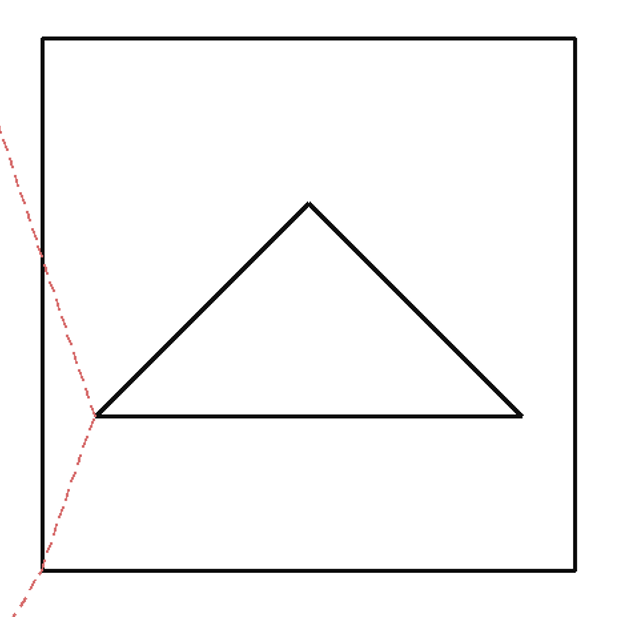
\includegraphics[width=\linewidth,height=0.23\textheight,keepaspectratio]{Figures/square-triangle-gcode-preview.png}\par(a) Commanded trajectory
\end{minipage}\hfill
\begin{minipage}{0.47\linewidth}\centering
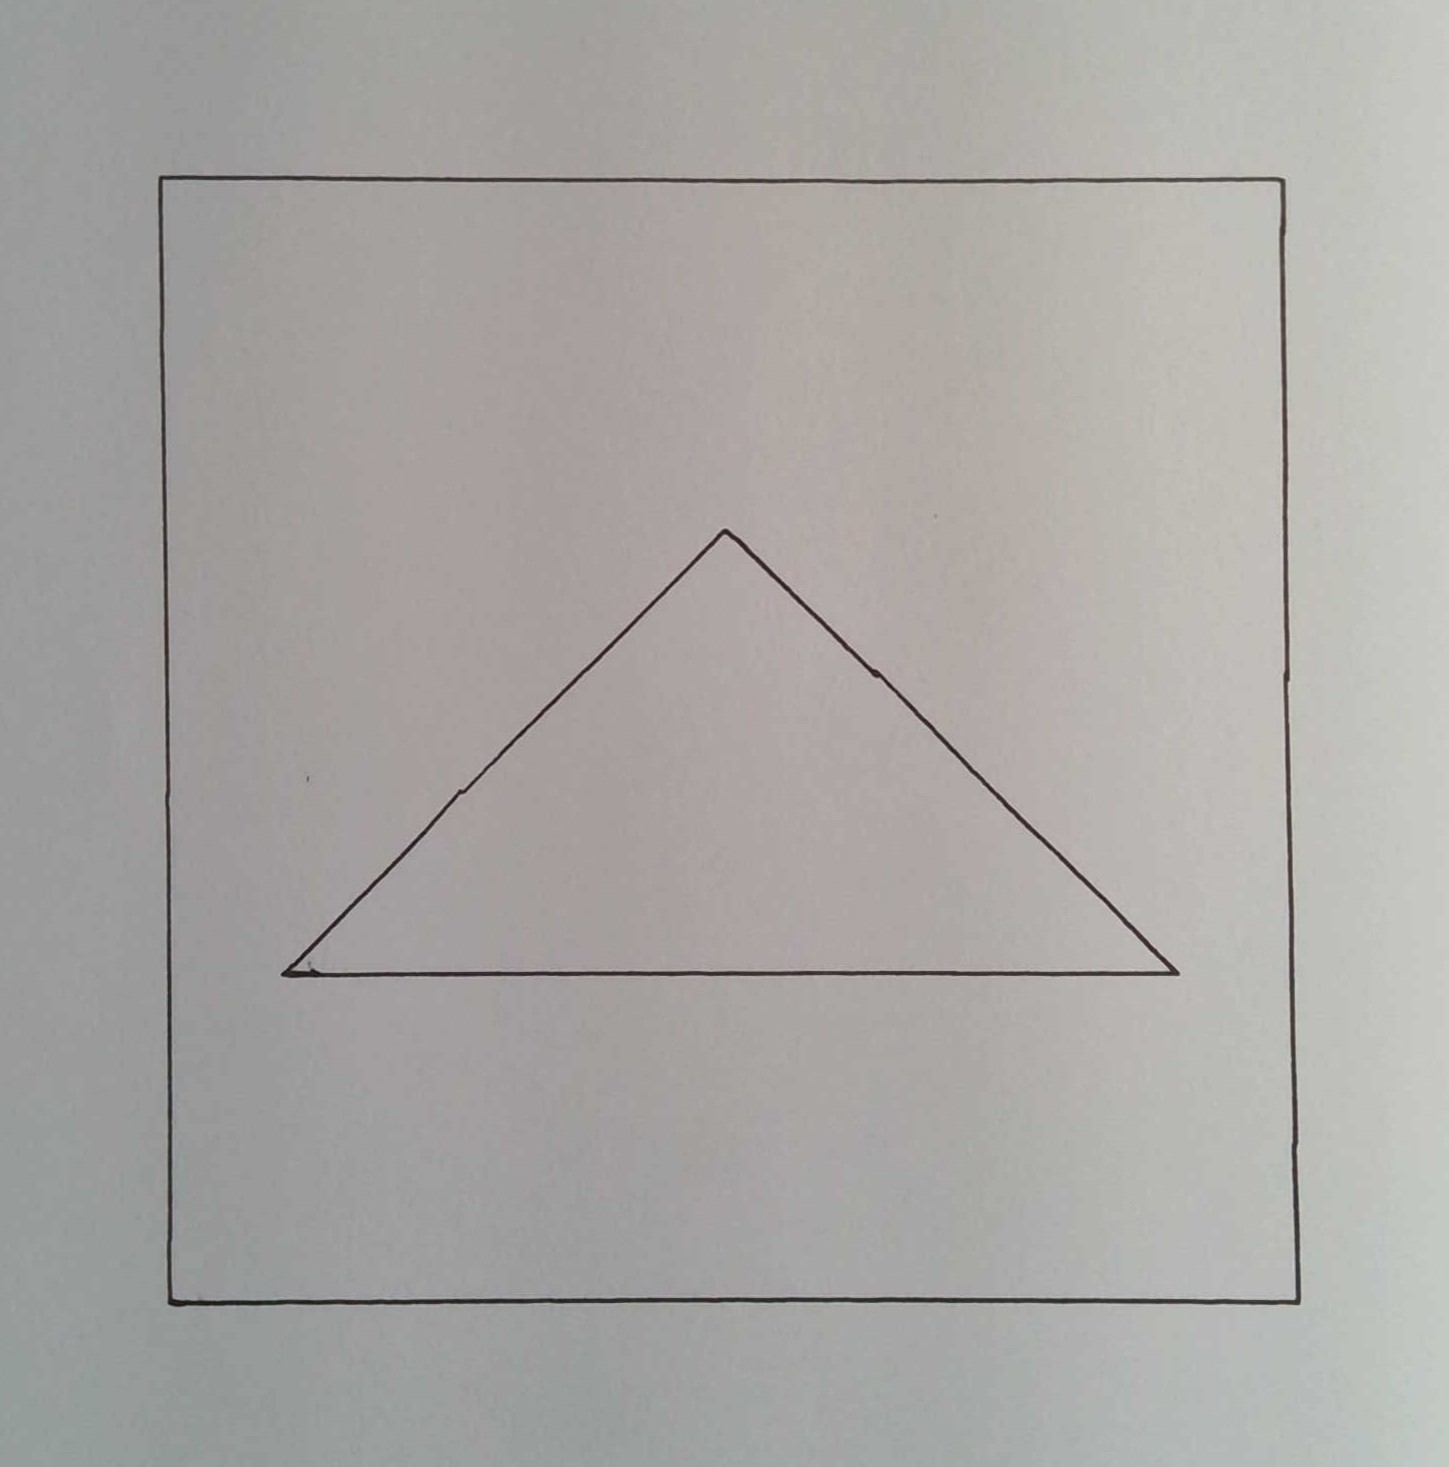
\includegraphics[width=\linewidth,height=0.23\textheight,keepaspectratio]{Figures/square-triangle-reproduced.jpg}\par(b) Physical drawing
\end{minipage}
\caption{Geometric commissioning example comparing the commanded path with the physical drawing. Formal positional qualification is reported in Results.}
\label{fig:des-shapetest}
\end{figure}

The design's principal strength is the direct relationship between orthogonal coordinates and motor displacement, combined with a mechanically shared drive on the two sides of the moving rail. Its principal uncertainties lie in physical compliance and open-loop execution. A missed step changes the actual position without changing the tracked count, and calibration cannot retrospectively recover where that happened. Controlled acceleration, a more consistent pulse scheduler and improved mechanical constraint are possible remedies, but their expected benefit must be separated from the performance of the implemented machine. The formal dimensional and repeated-drawing measurements in Results assess the resulting mechanical accuracy.
\FloatBarrier

\subsection{Page conditioning and line segmentation}
\label{sec:des-seg}
The recogniser requires an image containing one line of text. A photograph, however, may contain uneven illumination, a rotated page, printed rules, page edges and strokes extending between neighbouring lines. The purpose of this stage is to remove those disturbances while preserving the shape and relative spacing of the handwriting. The implemented sequence in \texttt{segment.py} works mainly on a half-resolution image, then returns to the full-resolution image to build the line crops.

\subsubsection{Input conditions and processing sequence}
The working image is a two-dimensional array of grey values. Where a colour array reaches the deskew routine, its channels are averaged to obtain brightness. Reducing the analysis image by averaging each $2\times2$ block reduces its pixel count by a factor of four. Averaging is preferred to selecting every second pixel because a thin stroke then contributes to the reduced image even if it falls between sampling positions. A further reduced mask is sufficient for the angle search, where only the arrangement of whole lines is needed.

The intermediate representations in Figure~\ref{fig:des-seg-stages} separate illumination correction, ink extraction, line boundaries and final crops. Inspecting these representations localises a missing stroke to the operation that removed it. The output includes the line images together with their order and diagnostic information such as skew angle, pitch and rejected crops.

\begin{figure}[!htbp]\centering
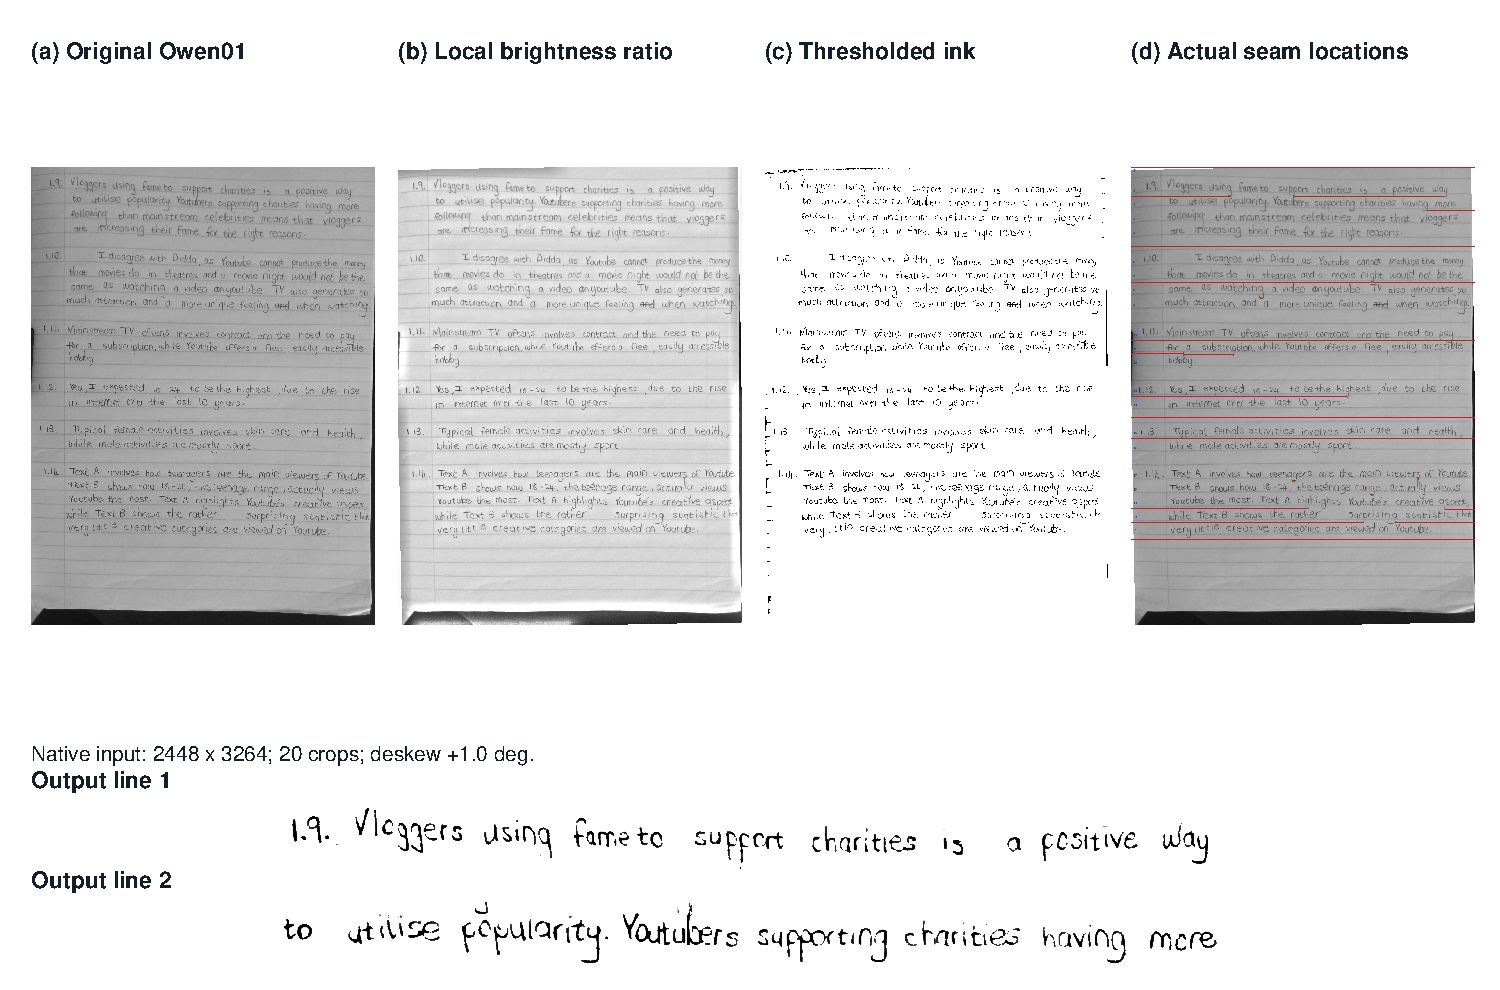
\includegraphics[width=0.96\linewidth]{Figures/design-segmentation-stages.pdf}
\caption{Processing stages used to obtain separate text-line images from a photographed page.}
\label{fig:des-seg-stages}
\end{figure}

A straight horizontal boundary is adequate only when there is a blank row between lines. Handwritten descenders and ascenders can overlap in vertical position without belonging to the same line. The chosen design first locates the lines, finds curved boundaries between them, then uses component geometry to refine which line owns each ink piece. This is more appropriate than treating every connected ink component as a character, since cursive words may form a single component.

Algorithm~\ref{alg:des-segment} links the representations used in Figure~\ref{fig:des-seg-stages}. The order matters: rules and artefacts are removed before estimating final line centres, whereas faint-ink recovery occurs after ownership has been established.

\begin{designalgorithm}
\caption{Photographed page to ordered line crops}
\label{alg:des-segment}
\prequire{Grey page on its chosen line axis.}
\pensure{Ordered full-resolution crops, coordinates and diagnostics.}
\begin{designpseudo}
\pstate{0}{$(G_f,G_h,M,R,\theta)\leftarrow\operatorname{Deskew}(G)$}
\pstate{0}{$M\leftarrow\operatorname{RemovePrintedStructure}(M,G_h)$}
\pstate{0}{$(M,\mathcal C)\leftarrow\operatorname{DropArtifactPieces}(M,R)$}
\pstate{0}{$(P,c)\leftarrow\operatorname{LineCentres}(M)$}
\pstate{0}{$b\leftarrow\operatorname{SeamCuts}(M,c,P)$}
\pstate{0}{$O\leftarrow\operatorname{AssignOwnership}(M,\mathcal C,b,c,P)$}
\pstate{0}{$\mathcal L\leftarrow\varnothing$; normalise full-resolution brightness}
\pstate{0}{\textbf{for each} line index $n$ \textbf{do}}
\pstate{1}{$C_n\leftarrow\operatorname{BuildLineCrop}(n,O,G_f,P)$}
\pstate{1}{\textbf{if} $C_n$ has sufficient ink and height \textbf{then}}
\pstate{2}{Append $C_n$, its fixed-canvas view and bounding box to $\mathcal L$}
\pstate{1}{\textbf{end if}}
\pstate{0}{\textbf{end for}}
\pstate{0}{$\mathcal L\leftarrow\operatorname{DropSolidCrops}(\mathcal L)$; renumber retained crops}
\pstate{0}{\textbf{return} $\mathcal L$, seams, ratio image and diagnostics}
\end{designpseudo}
\end{designalgorithm}

\subsubsection{Lighting normalisation and ink extraction}
The first requirement is to distinguish ink from paper under an illumination gradient. A single threshold applied directly to brightness can classify a shadowed part of the page as ink while losing pale strokes elsewhere. Local-mean comparison addresses this illumination problem in adaptive thresholding~\cite[pp.~2--3]{bradley2007}. The present design instead forms a local brightness ratio and selects its threshold from the ratio histogram. Equation~\ref{eq:des-ratio} compares each pixel with its own local background estimate instead.
\begin{equation}
R(y,x)=\frac{G(y,x)}{\max[B_r(y,x),1]},\qquad
M(y,x)=\mathbf{1}[R(y,x)<t^*].
\label{eq:des-ratio}
\end{equation}
In the Owen01 page trace, pixel $(y,x)=(317,343)$ of the $800\times600$ pre-deskew working image has $G=100$. Its 41 by 41 background window gives $B_r=161.43367$, hence $R=100/161.43367=0.619449$. The selected ratio threshold is $0.803906$, so this pixel enters the ink mask. The trace uses the documented reduction of the stored photograph.

Here $G$ is grey intensity on the 0--255 scale, $B_r$ is a square-window mean with radius $r$, $R$ is normalised brightness, and $M$ is the binary ink mask. The floor of 1 prevents division by zero in black regions. The code uses $r=\max(8,\min(40,\operatorname{round}(H/41)))$, where $H$ is the working-image height. The radius follows image size within bounded limits: it must average over strokes without following their darkness as if it were illumination.

The mean is evaluated through a summed-area table, using the four-corner rectangle sum described by Bradley and Roth~\cite[p.~2]{bradley2007}. For an exclusive prefix sum $S$, the window sum is obtained from four accesses, as shown in Equation~\ref{eq:des-integral}.
\begin{equation}
\Sigma_{[y_0,y_1)\times[x_0,x_1)}=
S(y_1,x_1)-S(y_0,x_1)-S(y_1,x_0)+S(y_0,x_0).
\label{eq:des-integral}
\end{equation}
The same pixel's four prefix values are $20696850$, $18404173$, $18359673$ and $16338366$. Equation~\ref{eq:des-integral} gives a window sum of $271370$, so $B_r=271370/1681=161.43367$. This is the local-background value used in the preceding mask decision.

The window area divides this sum to give $B_r$. Equation~\ref{eq:des-integral} makes the cost per window independent of its radius after the prefix image has been constructed. Edge replication is used by this local-mean routine so that the boundary is not darkened by artificial zero padding.

Otsu's criterion selects $t^*$ from the ratio histogram rather than from the original grey histogram~\cite{otsu1979}. Equation~\ref{eq:des-otsu} gives the between-class variance being maximised.
\begin{equation}
t^*=\arg\max_t\ \omega_0(t)\omega_1(t)
\bigl[\mu_0(t)-\mu_1(t)\bigr]^2.
\label{eq:des-otsu}
\end{equation}
For this page's ratio histogram, the selected bin is 171. Its masses are $\omega_0=0.07069375$ and $\omega_1=0.92930625$, with mean bin indices 124.98356 and 217.71913. Their between-class variance is approximately $564.97942$ in squared bin-index units. Converting the selected bin centre to the ratio scale gives $t^*=(171+0.5)(1.2/256)=0.80390625$, the threshold used above.

Here $\omega_0,\omega_1$ are the histogram masses below and above a candidate threshold and $\mu_0,\mu_1$ are their means. The normalisation in Equation~\ref{eq:des-ratio} first brings paper towards a common level, allowing the global criterion in Equation~\ref{eq:des-otsu} to operate on a more consistent image. The implementation uses 256 bins over the clipped ratio range 0--1.2.

Large solid regions are then removed because the dark surround or a binder interior can survive thresholding without representing handwriting. The page region is estimated from its bright connected area, and long nearly horizontal or vertical ink runs are masked as printed structure. Run thresholds are expressed relative to line pitch, rather than fixed photograph dimensions. The horizontal and vertical limits are respectively 1.25 and 1.4 pitches. These are geometric heuristics: a long handwritten underline can satisfy the same condition as a printed rule, so the algorithm is designed for text extraction rather than preserving every mark on a page.

\subsubsection{Page orientation and skew correction}
Orientation is treated at two scales. A quarter turn changes which axis contains the line gaps; a small skew changes how sharply ink is concentrated along rows. For the quarter-turn decision, the code compares the fraction of nearly empty rows in the current image and its $90^\circ$ rotation. A turn is accepted only when the rotated score exceeds the original by a factor of 1.35. This margin avoids rotating a page merely because two weak scores differ slightly. Sparse or unusually arranged text can still make the row-gap evidence ambiguous.

After choosing the line axis, the deskew routine tests angles from $-4^\circ$ to $+4^\circ$ at $0.5^\circ$ spacing. Equation~\ref{eq:des-skew} gives its objective, related to projection-profile methods~\cite{postl1986}.
\begin{equation}
\theta^*=\arg\max_\theta\sum_y p_\theta(y)^2,\qquad
p_\theta(y)=\sum_x M_\theta(y,x).
\label{eq:des-skew}
\end{equation}
The Owen01 angle search gave squared-projection scores of 442973 at $+0.5^\circ$, 464105 at $+1.0^\circ$ and 439403 at $+1.5^\circ$. The maximum over all seventeen tested angles was 464105, so the routine selected $+1.0^\circ$. These scores are computed from the reduced mask used by the angle search, before the final mask is rebuilt.

Here $p_\theta$ is the row ink count at a candidate angle. Squaring favours concentrated rows over the same amount of ink spread across many rows. Rather than rotating the complete mask for every trial, the implementation maps ink coordinates to candidate rows and counts them. The selected rotation is then applied to the full and working grey images, and the mask is recomputed. This avoids repeatedly interpolating a binary image.

A page and its upside-down version have the same line-axis structure. The server therefore uses the reader to compare up to three sampled line crops in both directions. It compares the mean best-frame log score, reuses the selected readings and reverses line order when necessary. This is an orientation heuristic, not an independent measure of text correctness. A reader that is confidently wrong can select the wrong orientation, particularly when little text is available.

\subsubsection{Line detection and separation}
The line pitch $P$ provides the main scale reference for later decisions. A smoothed row profile is formed from the central writing region; candidate peaks must exceed 6\% of its maximum. The preferred estimate is the median distance between peaks, subject to a lower bound based on component height. This check prevents the ascender, body and descender bands of a single large line from being treated as separate line spacings. Autocorrelation and a component-height estimate provide fallbacks when direct gaps are unsuitable.

Line centres are selected in order of peak strength, with a minimum separation of $0.6P$. This suppresses several peaks within the same line. The code also supports merging peaks separated by a shallow valley, but that additional rule is not automatically active for every photographed page; its default threshold disables merging. The distinction matters because a rule that improves rendered text need not improve the shadows and artefacts of a real photograph.

Between each pair of centres, a minimum-cost seam crosses the image from left to right. The dynamic programme in Equation~\ref{eq:des-seam} follows the seam-carving principle~\cite[p.~3]{avidan2007}.
\begin{equation}
D(y,x)=C(y,x)+\min_{|d|\leq s}
\{D(y+d,x-1)+0.02|d|\}.
\label{eq:des-seam}
\end{equation}
In the traced boundary between centres 38 and 61, the selected predecessor at column 283 changes from row 50 to row 49 in working-image coordinates. Its stored predecessor cost is $0.00641966$, the movement penalty is $0.02$ and the new local cost is $0.0000226843$. Equation~\ref{eq:des-seam} therefore gives $D\simeq0.00641966+0.02+0.0000226843=0.02644234$. This traces one selected minimum of the actual dynamic programme; equal-cost alternatives can also occur.

Here $D$ is accumulated cost, $C$ is the local cost and $s=7$ is the allowed row change per column. Backtracking from the minimum final cost returns the boundary. Equation~\ref{eq:des-seam} penalises unnecessary vertical movement while allowing a boundary to bend around a descender.

The project-specific cost in Equation~\ref{eq:des-seamcost} combines an ink-crossing penalty with a weaker attraction to the space between line centres. These terms adapt the minimum-cost seam principle to the detected text-line gaps; the weights are engineering choices examined by the sensitivity check below.
\begin{equation}
C(y,x)=4\widetilde M(y,x)
+0.012\left(\frac{y-y_m}{h_g}\right)^2.
\label{eq:des-seamcost}
\end{equation}
At that boundary point, $y_m=(38+61)/2=49.5$, $h_g=(61-38)/2=11.5$ and the closed mask is zero. The implemented local cost is therefore $C=0.012[(49-49.5)/11.5]^2=0.0000226843$. It provides the local term used in the preceding accumulated-cost calculation.

Here $\widetilde M$ is the mask after morphological closing, a dilation followed by erosion that fills narrow breaks and gaps~\cite[p.~541]{haralick1987}, $y_m$ is the midpoint of the neighbouring centres and $h_g$ is half their separation. The closing radius is $\max(2,\lfloor0.07P\rfloor)$ pixels. Closing fills narrow gaps that would otherwise let a seam enter a stroke, without simply treating a thick dilation around every letter as real ink. In Equation~\ref{eq:des-seamcost}, the midpoint term resolves low-ink alternatives; it is deliberately much weaker than the ink penalty. The examples in Section~\ref{sec:des-segverify} examine the resulting boundaries and the cases that still defeat these geometric preferences.

A new sensitivity check on six fixed gaps from two real pages varies the midpoint and step penalties separately. At the implemented 0.012/0.02 setting, mean midpoint offset is 0.363 working pixels; removing the midpoint attraction raises it to 4.055 pixels. All tested settings still cross two raw-ink pixels across those seams, so this checks the weights' effects rather than proving an optimum. Appendix~\ref{app:des-seam-sweep} gives the settings and retained outcomes.

Figure~\ref{fig:vt-seamfield} shows why the curved boundary is useful on Abhinav01 at native page resolution. Among that page's gaps, the first example was selected for the largest reduction in crossed ink: the midpoint cut intersects 64 working-image ink pixels, while the seam intersects one. The second was selected for the largest departure from the midpoint; its seam moves by up to 22 rows and crosses no ink, compared with 44 pixels for the straight cut. These selected examples expose the effect of the cost function rather than establishing an average segmentation improvement.

\begin{figure}[!htbp]\centering
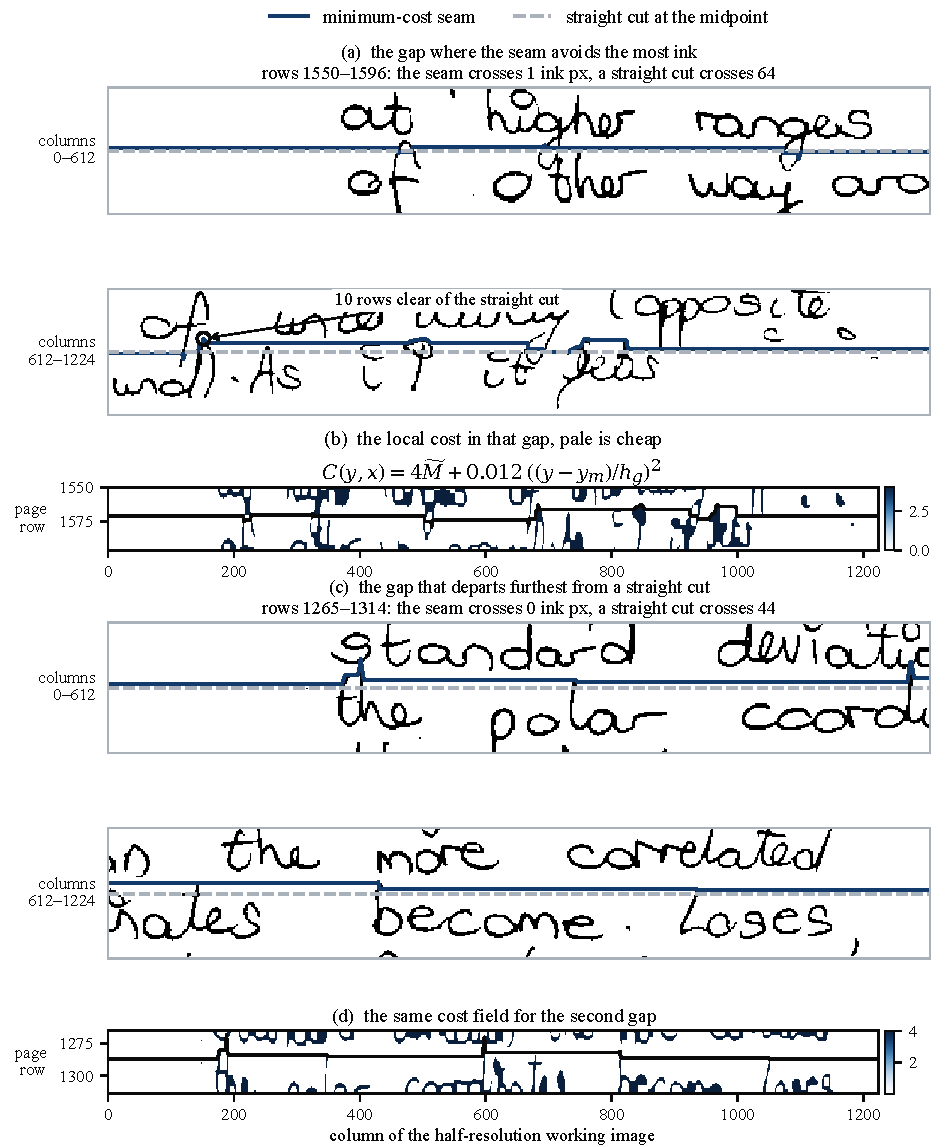
\includegraphics[width=\linewidth]{Figures/VisualTests/T25_seam_cost_field.pdf}
\caption{Seam paths and local cost fields on two explicitly selected gaps from Abhinav01.}
\label{fig:vt-seamfield}
\end{figure}

\subsubsection{Ink ownership and classifier crop preparation}
Seams initially divide the image into bands, but a pixel-by-pixel cut can separate a dot from its stem or clip a curved descender. Connected-component ownership therefore refines the band assignment. Components are found with row runs and union operations, following connected-component labelling principles~\cite[pp.~476--479]{rosenfeld1966}. The implementation includes diagonal contact, giving eight-connected components. Large pieces can still contain writing from more than one line, so component labelling alone is not a complete line assignment.

Algorithm~\ref{alg:des-ownership} summarises the correction order. For a component spanning several bands, a band holding at least 15\% of its in-band ink is substantial. The uppermost substantial band supplies the reference owner for small-piece corrections; otherwise the largest overlap is used. Large components are not indiscriminately moved into that band: their pixels retain seam-band assignment except where the small-piece and narrow-tail rules apply. This distinction preserves a word's main body while recovering a protruding part.

\begin{designalgorithm}
\caption{Refining seam bands into ink ownership}
\label{alg:des-ownership}
\prequire{Ink mask $M$, components $\mathcal C$, seams, centres and pitch $P$.}
\begin{designpseudo}
\pstate{0}{\textbf{for each} component $C\in\mathcal C$ \textbf{do}}
\pstate{1}{Count overlap $a_{C,n}$ with each seam band $n$}
\pstate{1}{$S\leftarrow\{n:a_{C,n}\geq0.15\sum_j a_{C,j}\}$}
\pstate{1}{Choose topmost $S$ as reference owner, or maximum overlap if $S=\varnothing$}
\pstate{1}{Correct eligible narrow tails and small pieces; reject remote specks}
\pstate{1}{Associate compact dots with plausible stems using pitch-scaled guards}
\pstate{0}{\textbf{end for}}
\pstate{0}{$O\leftarrow$ corrected ownership, preserving large-piece seam assignments}
\pstate{0}{\textbf{for each} raw component near a neighbouring line \textbf{do}}
\pstate{1}{\textbf{if} detached-dot or enclosed-ring guards pass \textbf{then}}
\pstate{2}{Transfer eligible pixels to the supported stem's line; protect correction}
\pstate{1}{\textbf{end if}}
\pstate{0}{\textbf{end for}}
\pstate{0}{Reassign residual fragments lacking their own body-band support}
\pstate{0}{\textbf{return} $O$; excluded pixels retain no line index}
\end{designpseudo}
\end{designalgorithm}

An \texttt{i} dot between two text lines illustrates the need for this sequence. A seam may put it with the upper line because of its vertical position, while a stem below supplies evidence for the lower line. Closing used for component analysis can also join the dot to an unrelated descender; the raw mask is therefore revisited rather than treating the closed component as unquestionable evidence. A ring-shaped mark needs the additional hole test so that an open hook is not treated as a detached loop. These are geometric decisions with ambiguous cases, rather than knowledge of the intended character.

The final crop is built from the full-resolution image and the refined ownership map. Contrast adjustment improves faint ink, while ownership restricts recovery so that strengthening one line does not simply pull a neighbouring stroke into it. The recogniser receives an aspect-preserving fit on a 64 by 640 canvas. Equation~\ref{eq:des-fit} defines the common scale for an original crop of height $h$ and width $w$.
\begin{equation}
a=\min\left(\frac{64}{h},\frac{640}{w}\right),\qquad
(h',w')\simeq(ah,aw).
\label{eq:des-fit}
\end{equation}
The archived first Owen01 line is $156\times2170$ pixels. Its fit scale is $a=\min(64/156,640/2170)=0.2949309$, giving a $46\times640$ resized image after integer rounding. The routine places it nine rows below the top of the 64-row canvas, retaining its aspect ratio and filling the remaining rows with white.

Remaining space is padded white, with the ink left-aligned and vertically centred. The shared scale in Equation~\ref{eq:des-fit} avoids stretching narrow letters differently from wide ones. Very long lines, however, become short in height when fitted to the width limit, which reduces the detail available to the networks.

The full-resolution crop uses a soft interpolation of its own ink mask to avoid jagged cut edges. A separate ownership exclusion is resized with nearest-neighbour interpolation: interpolating a yes/no ownership decision could partly return a neighbour's ink. Local thresholding can recover faint strokes within a neighbourhood of this line, but cannot recover ink already assigned to another line. Contrast is stretched between a robust ink level and paper level, followed by a darkness exponent of 0.55. This strengthens faint writing without replacing its geometry with a solid rectangular band.

The final solid-crop guard rejects a crop only when its dark-pixel fraction exceeds both 15\% and three times the page's median crop fraction. Requiring both prevents one unusually dense but genuine line from being rejected merely because other lines are sparse. This reduces the chance of a solid shadow receiving a strong writer vote in Section~\ref{sec:des-integration}. If every crop would be rejected, the implementation retains the input crop list; crop rejection is therefore a guard rather than a guarantee of valid text.

The three largest ownership corrections on Abhinav01 are displayed in Figure~\ref{fig:vt-ownership}. Colour identifies the assigned line, and the boxes locate pixels whose ownership changes after the component rules. Across the page, 462 pixels change assignment; the three boxed components contain 115, 78 and 73 pixels. The examples make the detached-piece and protruding-stroke corrections inspectable. No manually labelled pixel-ownership reference was supplied, so the reassignment count measures the action of the rules rather than their accuracy.

\begin{figure}[!htbp]\centering
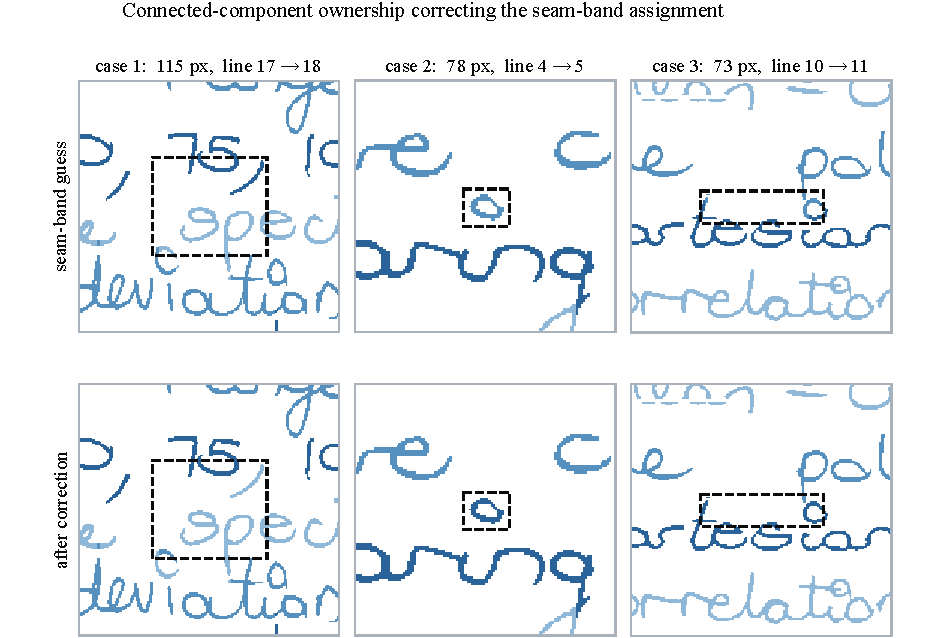
\includegraphics[width=\linewidth]{Figures/VisualTests/T27_ownership_corrections.pdf}
\caption{Initial seam-band ownership and corrected component ownership on the same page.}
\label{fig:vt-ownership}
\end{figure}

\subsubsection{Segmentation verification and limitations}
\label{sec:des-segverify}
Figure~\ref{fig:des-seg-variation} uses three actual photographs of the same three-line handwritten page from the camera roll. Their shadows and page presentation differ; no illuminance or physical rotation angle was recorded. The unchanged native images were processed through the line-axis decision and segmentation, without manually correcting an unsuccessful orientation.

The striped-shadow capture produced three crops. The diffuse-shadow capture produced four, so matching the writing visually remains necessary even under milder-looking illumination. The third capture was left on the wrong line axis: its gap scores were 0.379 and 0.400, giving a ratio of only 1.054 against the required 1.35, and segmentation produced 28 slices. Reaching the $-4^\circ$ deskew limit could not correct a missed quarter turn. These cases expose a sparse-page limitation of row-gap orientation; they do not establish a lighting operating range or a success rate. An acquisition guide or a separately verified orientation method would address the ambiguity before fine deskewing.

The fuller Owen page in Figure~\ref{fig:des-seg-stages} produced 20 crops at native resolution, matching its 20 labelled text lines. That count checks gross splitting, not every boundary pixel. Appendix~\ref{app:des-visual-tests} records the capture filenames, extended digital perturbations and independent algorithm checks, including failures after additional image reduction.

\begin{figure}[!htbp]\centering
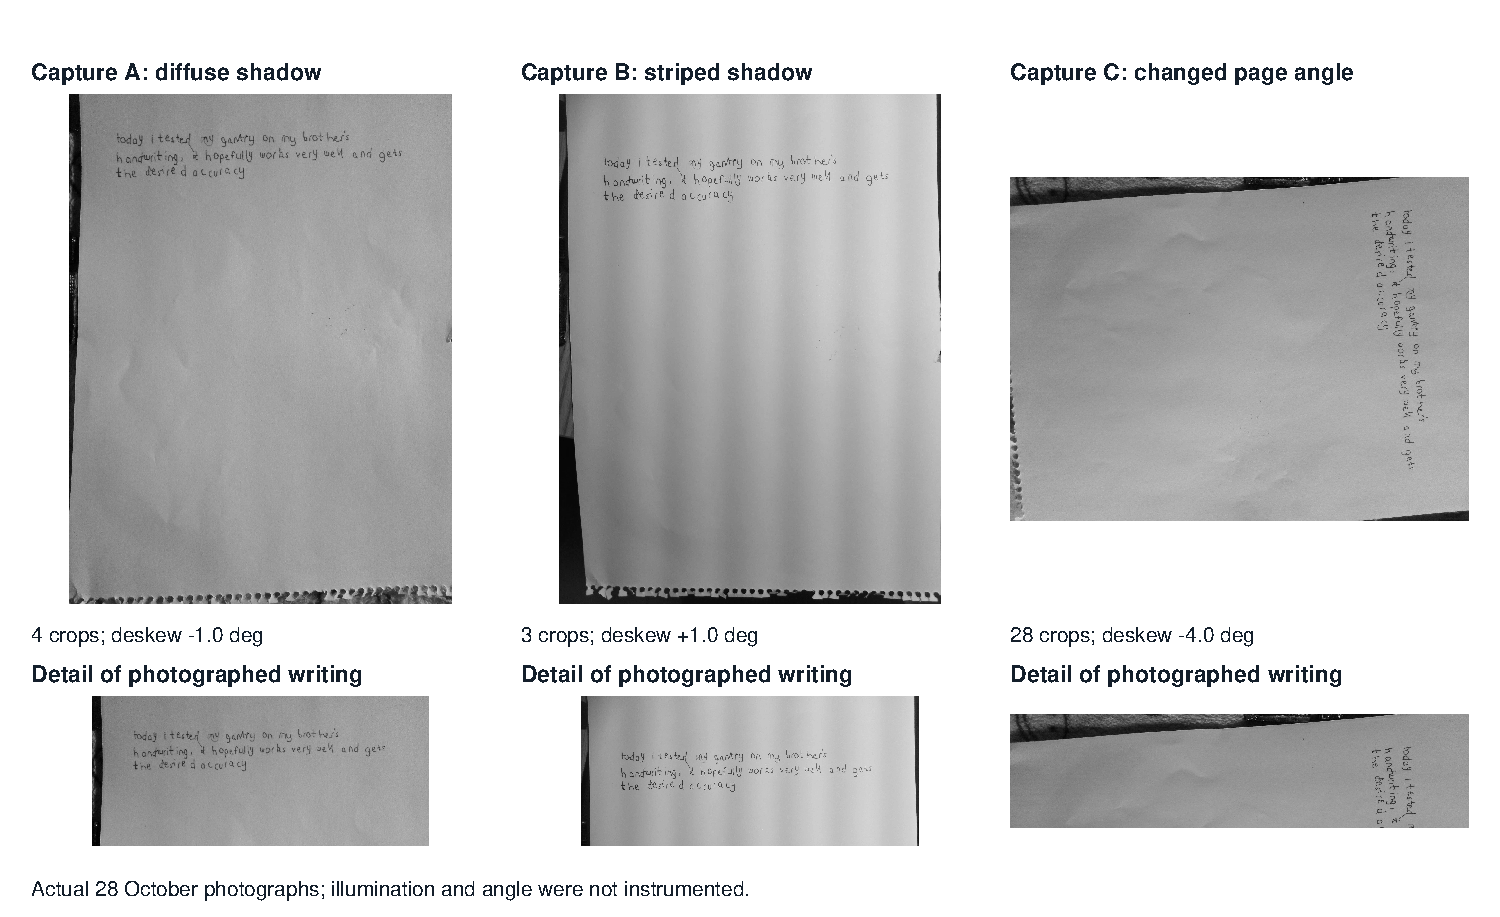
\includegraphics[width=0.95\linewidth]{Figures/design-segmentation-variation.pdf}
\caption{Actual repeated photographs and segmentation diagnostics for the same sparse page. Capture C retains the unsuccessful axis decision.}
\label{fig:des-seg-variation}
\end{figure}

The scale-based thresholds and curved boundaries accommodate changes in handwriting size and overlapping vertical extents without assigning every page a fixed pixel spacing. Their assumptions also define the limitations. Highly irregular line spacing weakens a single pitch estimate, touching strokes from two lines can defeat component ownership, and sparse pages provide weak orientation evidence. Severe perspective or page curvature is not corrected by a global rotation. Improving the mount addresses the latter at source; more general page rectification would add processing and require its own verification.
\FloatBarrier

\subsection{Neural network design, training and classification}
\label{sec:des-class}
The classification stage has two outputs: the text in a line and the identity of its writer. Both depend on stroke features, but text recognition must preserve their horizontal order while writer identification must combine evidence across the line. Two networks therefore use the same convolutional architecture with different heads. The recogniser follows the CNN--BiLSTM approach of Kizilirmak and Yanikoglu~\cite[pp.~4--5]{kizilirmak2023}; the project implements and integrates that architecture with its own preprocessing, training and handwriting-reproduction pipeline.

\subsubsection{Training data, labels and evaluation separation}
Public IAM handwriting~\cite{marti2002} and the photographed personal contributions provide examples with known text and writer identity. Public line images supply text-recognition training data, while writer-labelled pages and the personal samples support writer identification and style extraction. The eleven writers selected for the reported evaluation and intended demonstration are six database writers (150, 152, 153, 384, 552 and 588) and five personal contributors. A stored profile, a classifier output class and an evaluated writer are different objects; the checkpoint's recorded class mapping defines how its output indices are interpreted.

The data pipeline pairs every crop with its transcript and writer label. The same preparation functions are used by the first-principles and framework training routes so that a comparison does not silently change segmentation or label handling. Blank or unusable labelled lines are excluded. Characters outside the configured alphabet are filtered by the label encoder; they cannot be recognised as separate output symbols unless the alphabet and output layer are extended.

The page-based writer dataset holds out an IAM page per writer, while the personal data use a fixed-seed 15\% line split. A page split and a line split provide different separation: a held-out personal line can share camera conditions, page background and writing session with training lines. It is therefore appropriate to describe those samples as held-out lines, rather than as wholly unseen capture sessions. Augmented versions of a sample must remain within its assigned training partition.

Preparing public forms also requires excluding printed prompts and signatures before matching detected lines to their transcripts. The eleven-writer classifier corpus contains 1186 labelled lines: 517 IAM and 669 photographed lines, split into 1031 training and 155 held-out lines. The final reader instead uses a joint corpus of Teklia pre-cut IAM lines and the five photographed writers; its exact training and validation counts are not preserved in the available record.

Evaluation separation concerns three inputs: the writer classifier's training lines, the reader's training lines and the pages used to build glyph profiles. Holding a line out of one classifier does not exclude it from the other corpus, and constructing a profile from an evaluation page already exposes its letterforms. Cross-corpus source identifiers and profile-page manifests are therefore needed before describing combined performance as independent of those inputs.

\subsubsection{Shared convolutional feature extractor}
The input tensor has dimensions $(B,1,64,640)$, where $B$ is batch size. The grey crop is inverted and scaled to $[-1,1]$, making dark ink positive and white padding negative. Table~\ref{tab:des-backbone} gives the implemented feature-map dimensions. Two pooling operations reduce the width to 160 positions; there is no third spatial pooling stage before height is collapsed.

\begin{table}[!htbp]\centering\small
\begin{tabularx}{\linewidth}{|l|X|l|}
\hline\textbf{Stage}&\textbf{Operation}&\textbf{Output excluding batch}\\\hline
Input&Aspect-preserving line fit and intensity scaling&$1\times64\times640$\\\hline
1&Two $3\times3$ convolutions, each with batch normalisation and ReLU; $2\times2$ max pool&$32\times32\times320$\\\hline
2&Four convolution/normalisation/ReLU blocks; $2\times2$ max pool&$64\times16\times160$\\\hline
3&Six convolution/normalisation/ReLU blocks&$128\times16\times160$\\\hline
Height reduction&Maximum over the remaining height&$128\times1\times160$\\\hline
\end{tabularx}
\caption{Implemented convolutional backbone shared in architecture by the text and writer networks. The two models have separately trained parameters.}
\label{tab:des-backbone}
\end{table}

The convolutional feature extraction follows the reference architecture~\cite[pp.~4--5]{kizilirmak2023}. The local weighted-sum operation follows the CNN formulation~\cite[pp.~6--8]{lecun1998}; Equation~\ref{eq:des-conv} writes it explicitly for the numerical implementation. For output channel $o$, the input-channel and kernel sums combine into one feature value.
\begin{equation}
z_{o,y,x}=b_o+\sum_c\sum_{i,j}W_{o,c,i,j}X_{c,y+i,x+j}.
\label{eq:des-conv}
\end{equation}
For the first Owen01 line, channel 0 of the first convolution at canvas row 34, column 462 gives $\sum WX=-1.150897$ with learned bias $b=-0.000435125$. Equation~\ref{eq:des-conv} therefore produces $z=-1.151332$. The nine actual input and learned-weight values are retained in Appendix~\ref{app:des-real-calculations}.

Here $W$ is the learned kernel, $b$ its bias and $X$ the padded input. Equation~\ref{eq:des-conv} is the cross-correlation convention used by the implementation. Image patches are rearranged into a matrix and multiplied by flattened kernels, rather than evaluating a Python loop for every multiply. This follows the matrix formulation of convolution~\cite{chellapilla2006}. The choice improves the practicality of the numerical route while leaving the layer's calculation visible.

Batch normalisation evaluates Equation~\ref{eq:des-bn}, with channel statistics computed over the batch and spatial dimensions during training~\cite[pp.~4--5]{ioffe2015}.
\begin{equation}
\widehat z=\frac{z-\mu_B}{\sqrt{\sigma_B^2+\epsilon}},\qquad
y=\gamma\widehat z+\beta.
\label{eq:des-bn}
\end{equation}
At the same activation, the checkpoint stores $\mu=0.2163021$, $\sigma^2=0.02585394$, $\gamma=1.0193636$ and $\beta=0.1324657$. Using $\epsilon=10^{-5}$ in Equation~\ref{eq:des-bn} gives $y=1.0193636(-1.1513321-0.2163021)/\sqrt{0.02585394+10^{-5}}+0.1324657\simeq-8.53619$. The following ReLU sets this negative response to zero. These are the stored inference statistics, rather than statistics calculated from this single line.

Here $\gamma,\beta$ are learned channel parameters and $\epsilon$ stabilises division. At inference, stored running statistics replace $\mu_B,\sigma_B^2$, making Equation~\ref{eq:des-bn} a fixed affine operation. The following ReLU applies $\max(0,y)$ and max pooling retains the largest feature in each local window. These operations progressively convert pixel neighbourhoods into learned responses while reducing the spatial size passed to the task heads.

\begin{figure}[!htbp]\centering
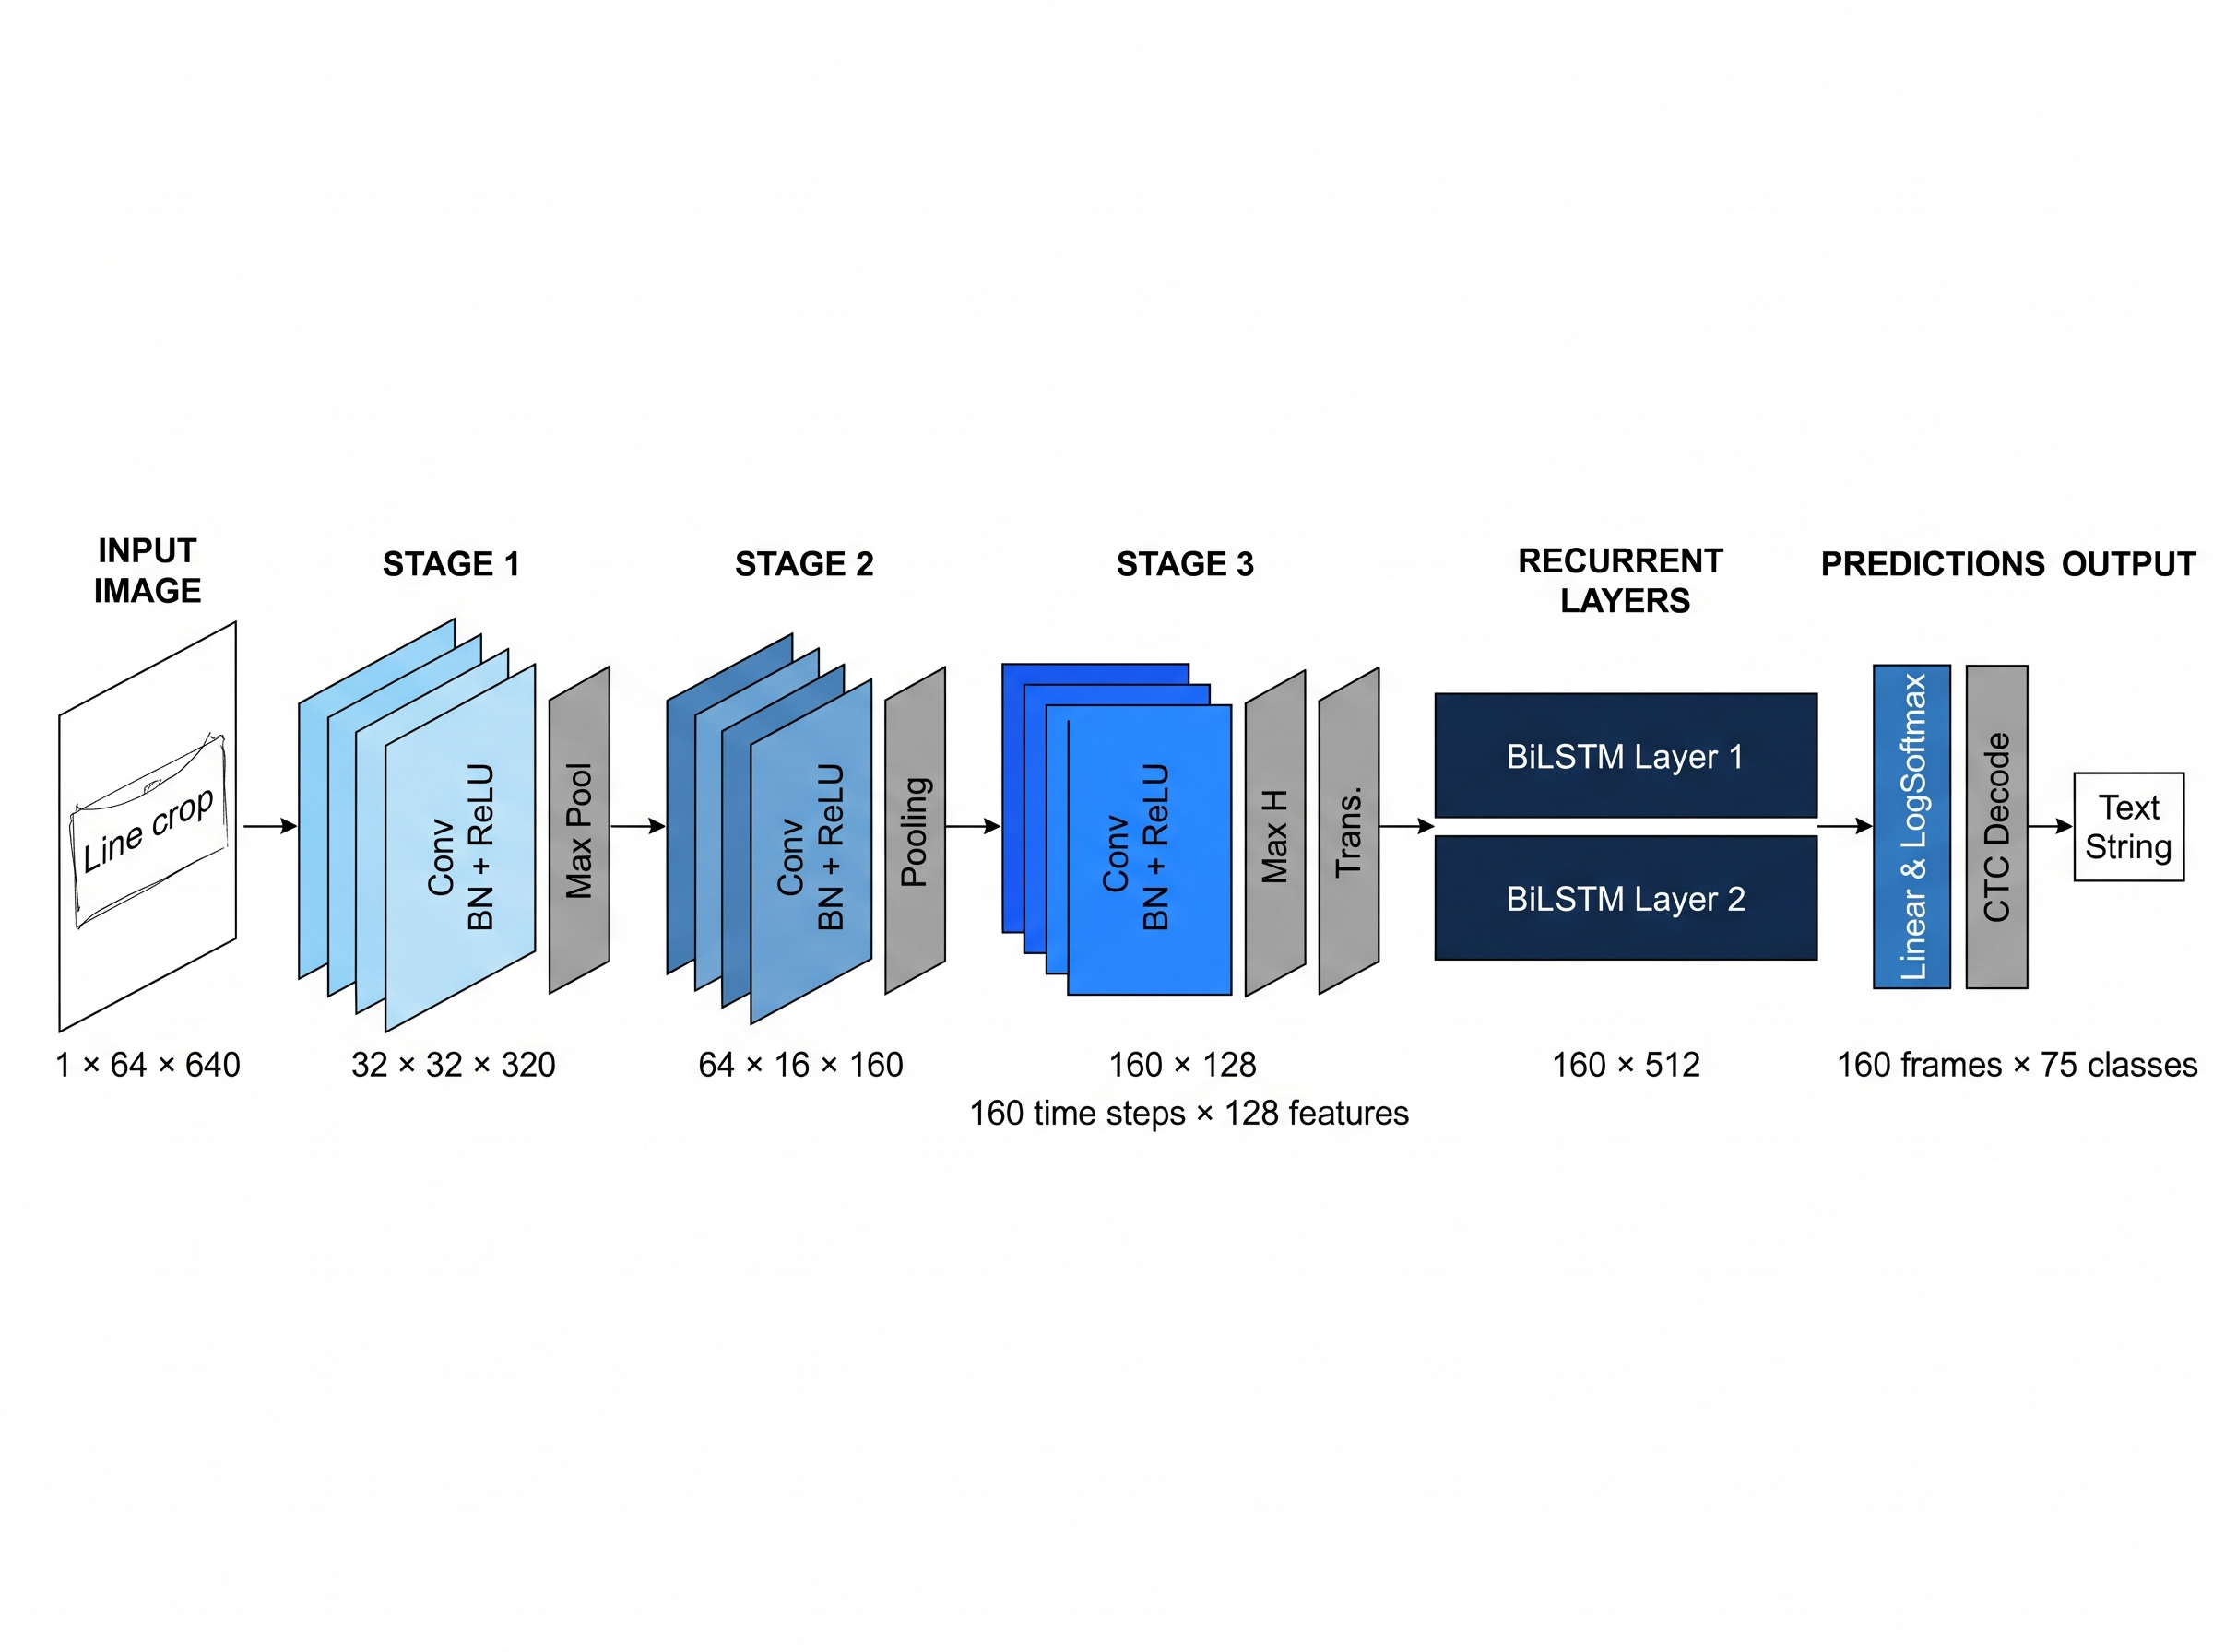
\includegraphics[width=0.96\linewidth,trim=0 130bp 0 134bp,clip]{Figures/BiLSTMCRNN.jpeg}
\caption{Architecture of the text reader and writer classifier.}
\label{fig:des-network}
\end{figure}

Figure~\ref{fig:des-network} makes the different uses of horizontal position explicit. The term ``shared'' refers to architecture and numerical building blocks; it does not mean that the trained writer classifier uses the reader's current weight tensors.

The arrays behind the architecture are shown in Figure~\ref{fig:vt-featurestack}, using the joint reader on the archived Owen line. Each row shows three channels selected for their activation strength at that stage; the maps are independently scaled for visibility, so their darkness is not a comparison of absolute response across layers. After the two spatial pooling stages, the final tensor is $128\times16\times160$. Taking the maximum over height gives $128\times1\times160$: 160 ordered feature columns, each containing 128 values. This links the convolutional representation to the sequence input without treating an output frame as a complete character.

\begin{figure}[!htbp]\centering
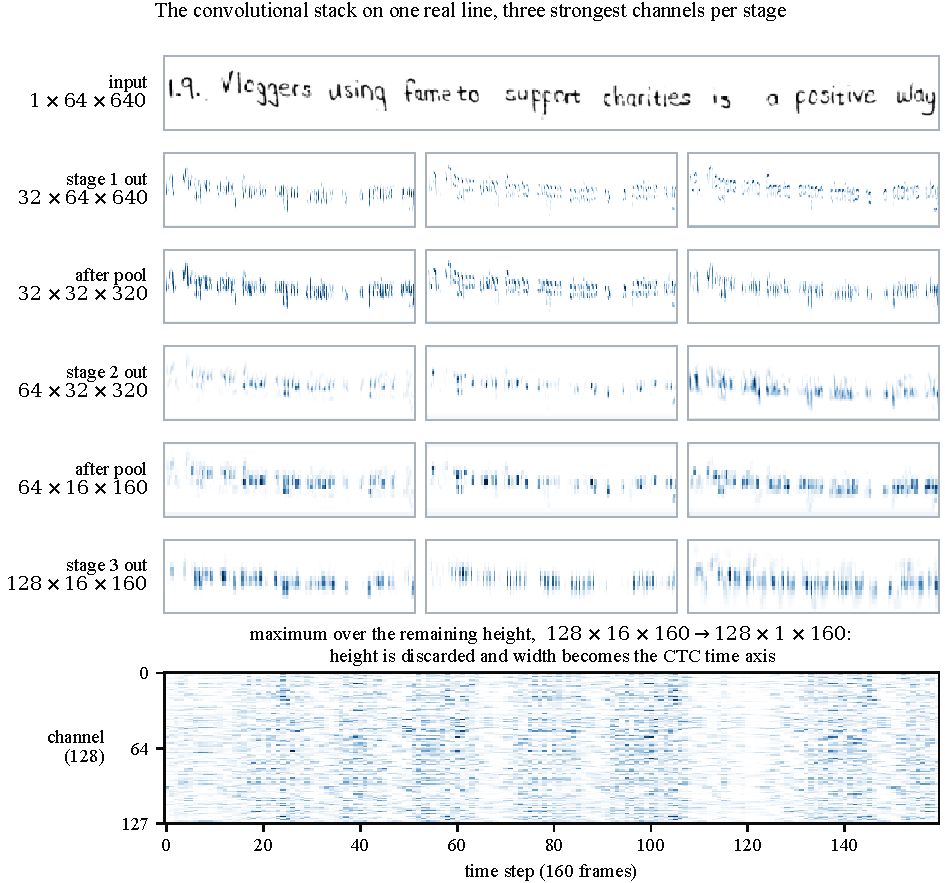
\includegraphics[width=\linewidth]{Figures/VisualTests/T32_feature_stack.pdf}
\caption{Feature maps and height pooling from a real line passed through the selected joint reader.}
\label{fig:vt-featurestack}
\end{figure}

\subsubsection{Text recognition using sequence modelling and CTC}
The text head treats the 160 feature columns as a sequence. Each column contains 128 features after height pooling. Two bidirectional LSTM layers, each with 256 hidden units per direction, combine evidence from both sides of a character before a linear head produces scores over the alphabet and the blank class. The configured alphabet contains 74 characters, giving 75 output classes including blank. The chosen input geometry and decoding are part of this project's implementation rather than an assertion that every setting in the reference study was reproduced.

The LSTM state update in Equation~\ref{eq:des-lstm} retains an additive memory path~\cite[p.~5]{graves2013}.
\begin{equation}
c_t=f_t\odot c_{t-1}+i_t\odot g_t,\qquad
h_t=o_t\odot\tanh(c_t).
\label{eq:des-lstm}
\end{equation}
In the first forward LSTM layer for that line, frame 10 and cell 0 have $c_{t-1}=-2.7277257$, $f_t=0.7306111$, $i_t=0.6666368$ and $g_t=-0.8560218$. Equation~\ref{eq:des-lstm} gives $c_t\simeq-2.5635625$. With $o_t=0.000145395$, the cell emits $h_t\simeq-0.000143680$. This records the memory calculation used while processing the real feature sequence.

Here $c_t$ is cell state, $h_t$ is hidden output, $i_t,f_t,o_t$ are sigmoid input, forget and output gates, and $g_t$ is the candidate update. Each is computed from the current feature vector and previous hidden state. The implementation omits the additional cell-to-gate peephole connections shown in the cited source. The backward direction applies the same type of recurrence to the reversed sequence, and the two outputs are concatenated. Equation~\ref{eq:des-lstm} explains why the implemented reader has sequence state in addition to convolutional features.

The gates are obtained from one matrix calculation, split in input, forget, candidate and output order: $[a_i,a_f,a_g,a_o]^T=W_xx_t+W_hh_{t-1}+b_x+b_h$. Sigmoid is applied to $a_i,a_f,a_o$ and $\tanh$ to $a_g$. Concatenating both directions gives 512 features per frame; the second recurrent layer therefore receives 512 inputs rather than the first layer's 128. At inference the entire line is available, so using right-hand context does not require predicting future input.

CTC trains from a line transcript without requiring character positions~\cite[pp.~2--3]{graves2006}. Equation~\ref{eq:des-ctc} sums the probabilities of frame paths that collapse to the target string.
\begin{equation}
\mathcal L_{\mathrm{CTC}}=-\log\sum_{\pi:\mathcal B(\pi)=\boldsymbol\ell}
\prod_{t=1}^{T}p_t(\pi_t).
\label{eq:des-ctc}
\end{equation}
For the complete labelled line ``1.9. Vloggers using fame to support charities is a positive way'', the recorded forward--backward total is $\log Z=-0.47033843$. Equation~\ref{eq:des-ctc} gives $\mathcal L_{\rm CTC}=0.47033843$ and $Z\simeq0.6247908$. This loss was evaluated offline from the trained reader's actual logits and known transcript, without updating its weights.

Here $p_t(k)$ is the frame probability for symbol $k$, $\boldsymbol\ell$ is the transcript, and $\mathcal B$ merges consecutive repeats before deleting blanks. For example, the path $a,a,\varnothing,b,b$ collapses to ``ab'', while $a,\varnothing,a$ preserves ``aa''. The dynamic programme uses blank-interleaved states with transitions that stay, advance one state, or skip a blank when the adjacent labels differ. Arithmetic is performed in log space to avoid multiplying many small probabilities.

The CTC collapse and best-path decoding rules follow Graves et al.~\cite[pp.~2--3]{graves2006}; the implementation produces $T=160$ frames. A target with $L$ labels and $r$ adjacent repeated-label pairs requires at least $L+r$ frames. The extended lattice has $2L+1$ states, but not every state must be visited; that number is not a universal minimum sequence length. At inference, greedy frame decisions are collapsed by the same rule. This avoids a dictionary or language model, but a locally plausible wrong frame path can remain wrong even where a beam search could recover an alternative.

Algorithm~\ref{alg:des-ctc} describes the numerical loss and derivative. Let $\alpha_{t,s}$ include the current state's emission, while $\beta_{t,s}$ accounts only for emissions after frame $t$. The derivative used by the implementation is then Equation~\ref{eq:des-ctcgrad}, with the occupancy convention obtained by adapting the CTC forward--backward derivation~\cite[pp.~5--6]{graves2006}.
\begin{equation}
q_{t,k}=\sum_{s:\ell'_s=k}\exp(\alpha_{t,s}+\beta_{t,s}-\log Z),
\qquad \frac{\partial\mathcal L}{\partial z_{t,k}}=p_t(k)-q_{t,k}.
\label{eq:des-ctcgrad}
\end{equation}
At frame 11, the probability of \texttt{V} is $p_{11,V}=0.98030665$ and the target-constrained occupancy is $q_{11,V}=0.99999995$. The CTC logit derivative is therefore $p-q=-0.01969329$. It is negative because the admissible target paths require more \texttt{V} probability than the current output supplies at that frame; the real-input finite-difference check in Appendix~\ref{app:des-expanded-checks} checks this derivative.

Here $Z$ is the total probability of admissible target paths, $z$ denotes logits and $q$ is posterior class occupancy. The convention for $\beta$ avoids counting the current emission twice. Equation~\ref{eq:des-ctcgrad} is averaged over the batch in the trainer, without an additional target-length division.
Algorithm~\ref{alg:des-ctc} in Appendix~\ref{app:des-training-procedures} gives the full forward--backward procedure with explicit blank/repeat transitions.

The word ``Vloggers'' in this actual transcript contains adjacent \texttt{g}s. They require separate emission runs with a blank between them: a direct skip between identical label states would collapse to one character. The same restriction is retained during forced alignment in Section~\ref{sec:des-alignment}; training sums admissible paths, whereas extraction selects one.

Figure~\ref{fig:vt-lattice} compares the two paths through the same reader output. Greedy decoding selects the largest probability at each frame, whereas forced alignment restricts the path to the supplied transcript, following the CTC conventions already defined above~\cite[pp.~2--4]{graves2006}. On this particular line, the decoded string matches the known transcript exactly; the blank class accounts for about 46\% of the mean frame probability. The repeated letters in ``Vloggers'' illustrate why separated emission runs are needed. This is one worked recognition example, not a replacement for the pooled character-accuracy results.

\begin{figure}[!htbp]\centering
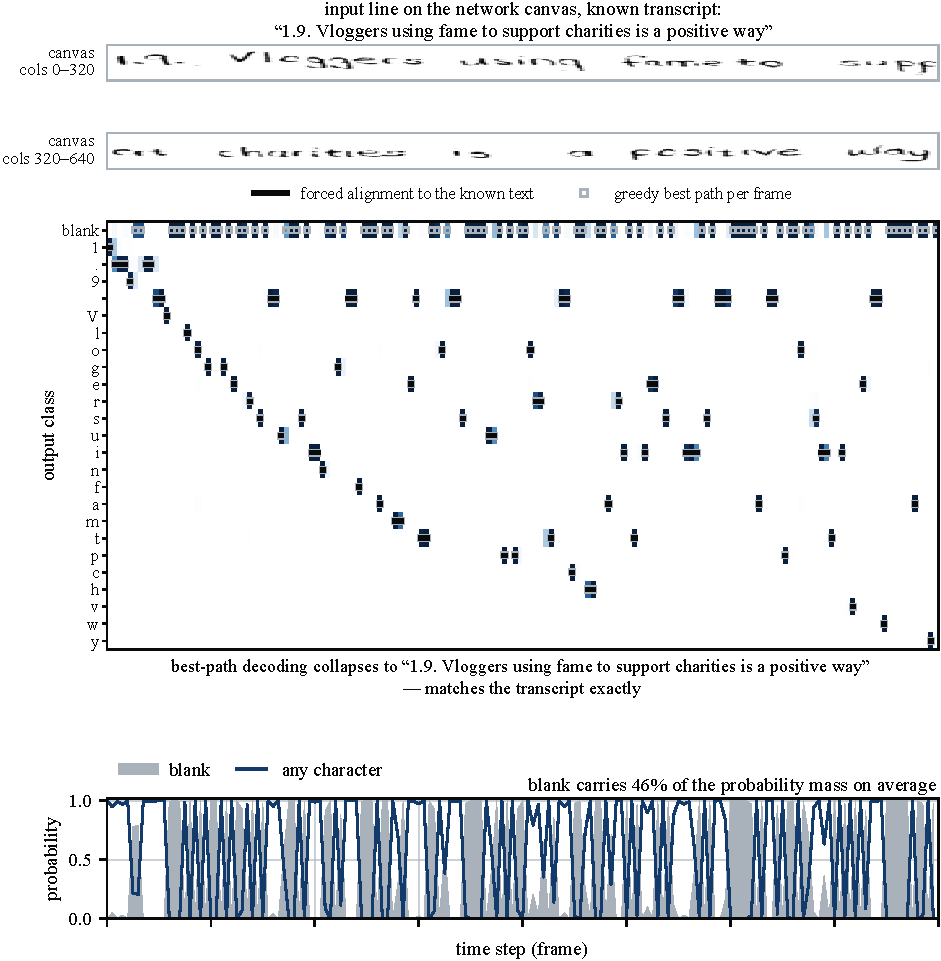
\includegraphics[width=\linewidth]{Figures/VisualTests/T36_ctc_lattice.pdf}
\caption{Forced alignment, greedy decoding and blank probability for one known Owen transcript.}
\label{fig:vt-lattice}
\end{figure}

\subsubsection{Writer identification and stroke normalisation}
\label{sec:des-shapenamer}
Writer identification should combine the shape evidence distributed along a line. It therefore averages the 160 column features rather than passing them through a sequence decoder. A 128-element feature vector is mapped through a 96-unit hidden layer, ReLU and a final $K$-class output. Dropout with probability 0.2 is active in the hidden head during training and omitted during inference~\cite[pp.~1931, 1934]{srivastava2014}. Here $K$ is the number of writers represented by that checkpoint.

The initial classifier operated on handwriting as photographed and performed well on those samples. Ink width can itself carry writer-identification information: Brink et al. explicitly use directional ink-trace width as a feature and relate it to the pen and writing style~\cite[p.~162]{brink2012}. The photographed input also retains darkness and capture variation, which the initial network was not constrained to ignore. The gantry uses its own pen, so reproducing the selected writer's geometry does not reproduce the same ink appearance. A classifier that relies on those cues would therefore provide an unsuitable basis for judging whether the robot preserved the writer's style.

The later classifier uses stroke-normalised input to restrict this source of variation. Ink is binarised, reduced to a centreline with Zhang--Suen thinning~\cite[p.~237]{zhang1984}, then expanded using morphological dilation~\cite[p.~533]{haralick1987} before the fixed-canvas fit. Equation~\ref{eq:des-strokenorm} combines these established operations with the project-selected width rule.
\begin{equation}
I_s=255\left[1-\delta_k\bigl(\operatorname{thin}(M)\bigr)\right],\quad
w=\operatorname{clip}\bigl(\operatorname{round}(\rho h_x),2,9\bigr),\quad
k=2\lfloor w/2\rfloor+1.
\label{eq:des-strokenorm}
\end{equation}
The same Owen crop has an estimated body-band height of 38 pixels. At the selected $\rho=0.17$, the width calculation gives $w=\operatorname{clip}(\operatorname{round}(0.17\times38),2,9)=6$, then $k=2\lfloor6/2\rfloor+1=7$. The actual redraw therefore uses a seven-pixel square dilation before fitting the line to the network canvas.

Here $h_x$ is estimated x-height, $\rho$ is the selected width fraction and $\delta_k$ is square dilation with an odd $k$-pixel kernel. The actual discrete kernel is important: nearby fractions can produce exactly the same transformed image. The code contains a default fraction of 0.14 and supports explicit training widths; the final model and its preprocessing must use matching settings.

The stroke-normalised classifier is used for writer identification and synthesis evaluation in the final design described here. This reduces dependence on ink appearance while retaining the letter geometry that the gantry can reproduce. It does not make the classifier completely independent of capture conditions, since thresholding and skeletonisation can themselves change a faint or touching stroke. It also removes potentially useful evidence from original handwriting, making the choice a deliberate trade-off between photograph-specific discrimination and consistency across original and reproduced writing.

Figure~\ref{fig:des-strokenorm} shows this transformation on existing real crops. The comparison makes the individual operations visible: binary extraction defines what ink is retained, thinning reduces it to a centreline, and dilation restores a controlled width. A matched ink-versus-shape comparison on original and reproduced samples can then test the reason for the choice without substituting classifier confidence for independent stylistic agreement.

\begin{figure}[!htbp]\centering
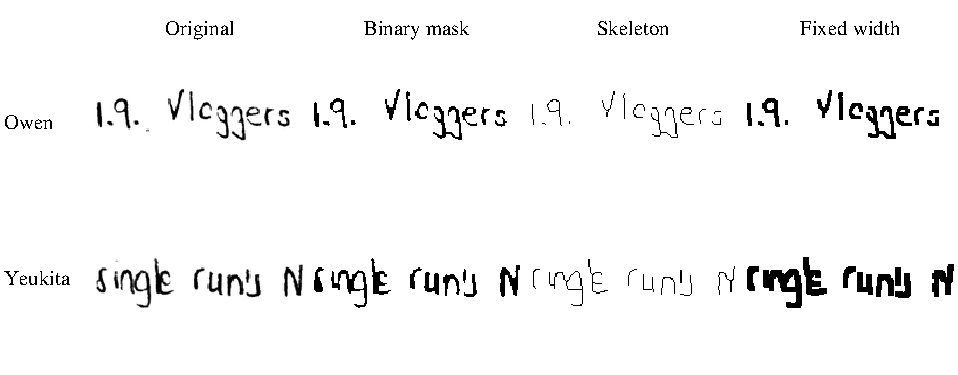
\includegraphics[width=0.98\linewidth]{Figures/design-stroke-normalisation.pdf}
\caption{Stroke-normalisation stages on selected Owen and Yeukita crops at the selected width fraction of 0.17.}
\label{fig:des-strokenorm}
\end{figure}

The width-selection tooling separates deterministic preparation from repeated learning. It skeletonises and redraws each crop once per candidate width, saving images together with writer names, labels and split membership. Training then augments those prepared images each epoch. A fixed split and controlled initialisation make the widths comparable without changing the writer population at the same time. The preparation code records cases where normalisation returns no usable ink and the raw crop is retained; these cases retain their original crop rather than a successfully normalised shape.

Table~\ref{tab:des-widthselection} records the supplied eleven-class validation sweep. All four runs had a 50-epoch budget and used the framework writer model on a Google Colab T4 GPU. The reported epoch is the best saved epoch, not the stopping epoch. The 0.17 setting gave the highest held-out accuracy in this sweep and defines the selected eleven-writer configuration; this is a preprocessing choice evaluated on validation data, not the integrated robot's writer-identification result.

\begin{table}[!htbp]\centering\small
\begin{tabular}{|c|c|c|}
\hline\textbf{Width fraction $\rho$}&\textbf{Best saved epoch}&\textbf{Held-out writer accuracy}\\\hline
0.06&38&98.06\%\\\hline
0.09&43&97.42\%\\\hline
0.11&39&98.06\%\\\hline
0.17&43&99.35\%\\\hline
\end{tabular}
\caption{Stroke-width selection using the same eleven-writer population and held-out partition.}
\label{tab:des-widthselection}
\end{table}

Appendix~\ref{app:vt-width} illustrates the actual integer dilation kernels selected by the sweep fractions; nearby fractions can coincide on a particular crop. The selected checkpoint stores its width as 0.17. Both preparation and inference for that configuration must use this value; the module default of 0.14 is not its training setting. Figure~\ref{fig:des-strokenorm} illustrates the selected transformation on existing crops. Reusing the held-out partition to choose width makes it model-selection data; an independent test set remains necessary for an unbiased final performance claim.

\subsubsection{Training procedure and model selection}
\label{sec:des-training}
The implemented training routes update the convolutional backbone and task-specific head together. Convolution weights use variance-scaled initialisation; normalisation scales begin at one and offsets at zero. Training-time augmentation changes line geometry while preserving its label. The implemented transforms include shear, small rotations, perspective changes and elastic distortion. These operations are applied only to the training view, while validation retains a consistent preprocessing path.

The text trainer supports public lines, page-derived lines and a joint source that mixes public and personal examples. In the joint configuration, a personal-sample fraction controls their representation rather than letting a much larger public dataset determine the entire batch distribution. The default fraction is 0.20. This is a sampling choice, not a claim that personal and public samples are interchangeable. Its value and the training source must accompany any comparison between checkpoints.

Table~\ref{tab:des-training} summarises the numerical training recipe exposed by the current implementation. The number of epochs is a run setting and should be reported from the actual training record, rather than taking a command-line default as the completed run.

\begin{table}[!htbp]\centering\small
\begin{tabularx}{\linewidth}{|l|X|X|}
\hline\textbf{Setting}&\textbf{Reader}&\textbf{Writer classifier}\\\hline
Objective&CTC loss&Cross-entropy\\\hline
Optimiser&RMSprop&AdamW\\\hline
Initial learning rate&$10^{-3}$ default&$10^{-3}$ default\\\hline
Weight decay&$10^{-5}$&$10^{-4}$\\\hline
Learning-rate schedule&Plateau reduction, factor 0.5, patience 5, minimum $10^{-5}$&Cosine annealing over the configured run\\\hline
Gradient-norm clipping&Not applied by the current NumPy text loop&Maximum norm 5\\\hline
Best-checkpoint criterion&Lowest validation loss&Highest validation accuracy\\\hline
\end{tabularx}
\caption{Training settings implemented in the first-principles trainer. The table describes implemented defaults rather than a recovered record of every completed training run.}
\label{tab:des-training}
\end{table}

Cross-entropy penalises the writer model's predicted probability of the true class. For label $y$ and probabilities $p_k$, its per-sample loss is $-\log p_y$, with logit derivative $p_k-\mathbf{1}[k=y]$~\cite[p.~6]{graves2013}. The CTC backward pass similarly relates each predicted frame probability to its target-state occupancy, calculated by forward and backward recurrences through the alignment lattice~\cite[pp.~4--6]{graves2006}. These gradients are propagated through the task head and the convolutional stages; they are not supplied to the numerical trainer by automatic differentiation.

Validation runs with dropout disabled and stored normalisation statistics. A low training loss alone does not select the model. Separate checkpoint and best-model files preserve progress while retaining the selected validation model. Reproducible batching, declared splits and saved writer mappings support later evaluation, but comparable recipes do not imply identical weights or learning curves across implementations.

Algorithm~\ref{alg:des-train} identifies the operations actually required for a first-principles training batch. Forward caches store quantities needed by the derivatives, rather than rerunning stochastic augmentation or dropout during the backward pass.
The complete numerical batch/update procedure appears in Algorithm~\ref{alg:des-train} in Appendix~\ref{app:des-training-procedures}; the calculations remain explicit in the source.

\subsubsection{First principles and framework implementations}
\label{sec:des-implementations}
The first-principles route in \texttt{train.py} evaluates the forward pass, backward pass, loss and optimiser updates using explicit NumPy operations. NumPy supplies array arithmetic and matrix operations; it does not supply a convolutional network, automatic differentiation or a CTC training function in this route. The learned parameters are stored as named arrays. The inference module reads these arrays and evaluates the forward operations without requiring a machine-learning framework.

The framework route in \texttt{trainlibrary.py} expresses the corresponding networks using PyTorch layers and automatic differentiation. Both routes use the project's data preparation, parameter naming and named-array export layout. This makes the framework implementation useful as a numerical reference while allowing either training route to supply weights to the NumPy inference code.

The selected reader and eleven-writer weights were trained using PyTorch and exported to named arrays. The first-principles contribution comprises the implemented numerical training operations and the operational NumPy forward path. Fixed-parameter comparisons verify the numerical calculations; the provenance of the selected weights remains the framework training route.

Matching the architecture is not sufficient to establish a matched training experiment. The current numerical CTC function averages unnormalised sequence losses across the batch, whereas the framework trainer constructs CTC with its default mean reduction, which normalises each sequence by target length before averaging~\cite{pytorchctc}. The framework loop also zeroes impossible-alignment losses. These conventions must be matched for a controlled training comparison because target-length weighting changes the influence of short and long lines. Named-array export remains compatible with both routes.

The selected demonstration reader is \texttt{paper\_cnn\_bilstm\_ctc\_joint\_best.npz}; the selected eleven-writer checkpoint is \texttt{author\_shape\_11\_pw170\_weights.npz}. Results in Section~\ref{sec:results} compare these selected models with separately trained numerical-route reader and writer checkpoints. The joint reader also supplies the numerical Design traces, so those traces retain their original checkpoint provenance. The reader's training computer, completed epoch count and original learning-rate/batch settings are not preserved in the supplied record. The implementation defaults in Table~\ref{tab:des-training} must therefore not be presented as recovered settings for that historical run.

The operation-by-operation comparison is retained in Table~\ref{tab:des-implementations}, Appendix~\ref{app:des-reference-tables}.

Equation~\ref{eq:des-conv} and the shape progression in Table~\ref{tab:des-backbone} define the implemented forward calculation. Its numerical correspondence and the backward operations are checked separately in Section~\ref{sec:des-netverify}. This separation distinguishes a correct description of an architecture from evidence that its calculations were implemented correctly.

The patch-matrix weight/input derivatives, their algebraic derivation and the patch-storage calculation are given in Appendix~\ref{app:des-expanded-checks}.

Additional convolution and CTC derivative checks are illustrated in Appendix~\ref{app:vt-gradient}; they test numerical operations separately from recognition accuracy.

\subsubsection{Network verification and design limitations}
\label{sec:des-netverify}
Verification separates numerical correspondence from learning performance. For the first, the implementations receive the same parameters and inputs, with matched precision, normalisation state and stochastic masks. Differences in logits, loss and gradients then test the implementation. A second experiment trains each route on the same split with recorded initialisation and settings, and compares learning behaviour and held-out predictions. These experiments answer different questions: separately trained weights can differ even when the underlying operations agree.

The existing comparison archive contains a controlled text experiment using 500 training lines, 40 validation lines and 40 test lines over 15 epochs. It is useful supporting evidence for the implementation, but it is not the final eleven-writer system evaluation. A separate archived double-precision comparison uses two random 64 by 640 inputs and identical initial weights, checking the reader and a thirteen-output writer head. Table~\ref{tab:des-numericalcheck} summarises its recorded values. The writer dropout is disabled for this comparison so that unrelated random masks do not dominate the difference.

\begin{table}[H]\centering\small
\begin{tabularx}{\linewidth}{|X|r|r|}
\hline\textbf{Recorded comparison metric}&\textbf{Reader}&\textbf{Writer classifier}\\\hline
Maximum logit difference / maximum magnitude&$2.12\times10^{-14}$&$3.04\times10^{-15}$\\\hline
Absolute loss difference&$1.14\times10^{-13}$&$1.78\times10^{-15}$\\\hline
Worst ranked gradient relative $L_2$ difference&$2.80\times10^{-13}$&$6.01\times10^{-14}$\\\hline
\end{tabularx}
\caption{Archived float64 implementation comparison from the CleanPipeline2 verification script. This is a controlled numerical check, not a final-model recognition result.}
\label{tab:des-numericalcheck}
\end{table}

The logit metric in Table~\ref{tab:des-numericalcheck} divides the largest absolute difference by the larger maximum magnitude, with a $10^{-8}$ denominator floor. Gradient differences are $\|g_N-g_T\|_2/\|g_T\|_2$, where $g_N$ and $g_T$ are numerical-route and framework gradients. Tensors whose maximum gradient magnitude is below $10^{-6}$ are retained in the archive but excluded from the worst-ranked summary: dividing roundoff by a nearly zero gradient gives an unhelpful relative error. These results support close agreement for that tested configuration; they do not establish equivalence for every input, code revision or training trajectory.

A separate, newly run small-lattice check enumerated all $4^5=1024$ frame paths for a repeated-label target and compared their summed probability with the numerical CTC loss. The absolute loss difference was $4.44\times10^{-16}$; central differences over all 20 logits gave a maximum absolute derivative difference of $3.63\times10^{-11}$. This verifies that finite example, including the required blank between repeated labels. Its construction and limits appear in Appendix~\ref{app:des-visual-tests}; it is not a learned-model accuracy measurement.

The finite-difference reference, numerical substitution and its treatment of non-smooth operations are recorded in Equation~\ref{eq:des-gradcheck} in Appendix~\ref{app:des-expanded-checks}.

The main design limitations concern what the input and training population can support. Fixed-width fitting limits detail in long lines; a closed writer head always selects among its trained classes; and line-level personal holdout does not establish independence from page or capture conditions. Stroke normalisation improves consistency with the pen plotter but can destroy detail when thresholding or thinning fails. These limitations should be assessed through appropriate examples and held-out measurements, rather than by treating a high softmax probability as proof of generalisation. Formal recognition and writer-identification qualification remains in Results.
\FloatBarrier

\subsection{Style extraction and handwriting reproduction}
\label{sec:des-reproduction}
Recognising a line does not provide the motion needed to write it. The reproduction stage must recover usable pen paths from a writer's examples, store the properties that distinguish that writer, and assemble the paths into text that was not necessarily present in the examples. The chosen representation is a library of normalised glyph trajectories accompanied by line-level style measurements. Profile extraction and trajectory assembly are implemented in \texttt{style.py} and \texttt{synthesise.py}, respectively. This representation provides explicit control over scale and movement, while making the limits of character-based reproduction visible.

\subsubsection{Choice of reproduction representation}
The available writer samples are a few labelled pages photographed after writing. A glyph library can reuse these observations without fitting a separate generative network for each writer. Haines et al. provide a relevant precedent: their standard experiments used approximately four A4 pages per writer~\cite[p.~4]{haines2016}. This is evidence that a small-page collection can support a glyph-based approach, not a guarantee that four pages cover every character or writing context. The present library likewise depends on the characters and variants actually observed.

The offline data also influenced the choice. Graves's recurrent synthesis model learns from ordered pen positions and end-of-stroke markers~\cite[p.~18]{graves2013}; these are not recorded in this project's photographs. A skeleton supplies geometric paths, but cannot recover their true order, speed or pressure. Using it as measured online training data would introduce an unsupported assumption.

Learned image generators remain a valid alternative, including methods that need very few references from a new writer. For example, One-DM uses one style reference at generation, but its IAM experiment trains with 339 writers and its implementation uses four RTX 3090 GPUs~\cite[p.~9]{dai2024}. A small reference set must therefore be distinguished from the corpus and computation needed to train the generator. Developing and training an additional generator from first principles on the ODROID was outside the chosen computational scope; no training-time comparison was measured. The glyph approach instead retains explicit trajectories that can be scaled, joined and converted directly to machine coordinates. Its trade-off is weaker modelling of connected, context-dependent letterforms, examined at the end of this subsection.

\subsubsection{Character alignment and glyph extraction}
\label{sec:des-alignment}
The extraction input is a line image and its known transcript. Character boundaries are not supplied as labels. The alignment builds on the blank-interleaved CTC lattice~\cite[pp.~4--5]{graves2006}. Instead, the trained reader gives a probability distribution for every output frame, and forced alignment finds the highest-scoring CTC path consistent with the supplied text. This is a localisation problem: the transcript constrains which labels must occur, while the frame scores indicate where they most plausibly occur.

The alignment uses the same permitted transitions as the CTC training lattice, but maximises a path score instead of summing all path probabilities. Equation~\ref{eq:des-viterbi} gives the recurrence by replacing path summation in the CTC lattice with maximisation~\cite[pp.~4--5]{graves2006}.
\begin{equation}
V(t,s)=\log p_t(\ell'_s)+\max_{r\in\mathcal P(s)}V(t-1,r).
\label{eq:des-viterbi}
\end{equation}
For the \texttt{V} in that Owen line, frame 11 corresponds to state 11 of the blank-interleaved transcript. Its log emission is $-0.01988991$ and the three admissible predecessor scores are $-13.91888$, $-10.01139$ and $-1.3624485$. Equation~\ref{eq:des-viterbi} selects their maximum and gives $V=-0.01988991-1.3624485=-1.3823384$. Backtracking assigns \texttt{V} the frame interval $[11,12)$.

Here $\ell'$ is the blank-interleaved transcript and $\mathcal P(s)$ is the permitted predecessor set: stay, advance one state, or skip an admissible blank. Backtracking yields the frames assigned to each character. Equation~\ref{eq:des-viterbi} makes clear why correct text does not guarantee correct boundaries: several spatial allocations can remain plausible under the same transcript.

An output frame is converted through the network canvas to the original crop using the inverse of its aspect-preserving scale. If a frame edge is $t$ out of $T$ and the crop was scaled by $a$, its initial horizontal location is approximately $(640t/T)/a$, clamped to the source width. This undoes the resize rather than assuming that every crop occupied the complete 640-pixel width.

The baseline and x-height are operational estimates from the line's horizontal ink profile, not annotated typographic measurements. With $p(y)=\sum_x M(y,x)$, the implementation takes the first and last rows satisfying $p(y)\geq0.45\max p$ as the body-band top and baseline; their difference gives $h_x$. Bands below three pixels are rejected. This common scale makes glyph dimensions comparable across source resolutions, although unusual capitals, short lines or a large descender can bias the estimated body band.

The worked example in Figure~\ref{fig:des-alignment} uses an archived original Owen line crop, visually matched to the first line of its page transcript, with the joint reader checkpoint. The reader recovered the full line, and the extraction routine then generated the displayed boundaries and normalised paths. Correct text does not certify a correct individual cut: small punctuation and neighbouring strokes still require inspection. The archived crop is identified separately from the new whole-page segmentation run in the evidence manifest.

The initial boundaries are refined by looking for thin, low ink near the expected cut. Equation~\ref{eq:des-cutcost} defines the project-specific column cost used for this refinement. It combines low ink density with a preference for cutting a shallow connector near the baseline.
\begin{equation}
C_x=\frac{\overline p_x}{q_{0.60}(\{\overline p_j:\overline p_j>0\})}
+1.15\operatorname{clip}\left(\frac{b-y_{\mathrm{top}}(x)}{h_x},0,3\right).
\label{eq:des-cutcost}
\end{equation}
The refined right boundary of this \texttt{V} is source column 193. Although smoothing gives $\overline p_{193}=2.8$ and the positive-column reference is 14.36, the raw ink count at column 193 is zero. The explicit blank-column rule therefore overrides $2.8/14.36$ and assigns zero cut cost. This is a real case in which the gap rule prevents smoothing alone from penalising a clean separation.

Here $\overline p_x$ is smoothed column ink count, the denominator is its 60th percentile over positive counts, $b$ is baseline position, and $y_{\mathrm{top}}(x)$ is the highest ink row in that column. A denominator floor prevents division by zero. A true blank column is assigned zero cost. The search radius is approximately half an x-height, with a smaller penalty for distance from the initial boundary. The two terms in Equation~\ref{eq:des-cutcost} favour a narrow connector near the baseline over cutting through the body of a letter.

One shared boundary array is enforced to remain increasing, with a minimum cell width of $\max(1,0.08h_x)$ pixels. Independently snapping neighbouring boundaries could place both at the same gap and create an empty glyph. Figure~\ref{fig:des-alignment} shows the refined cuts and resulting character shapes.

\begin{figure}[!htbp]\centering
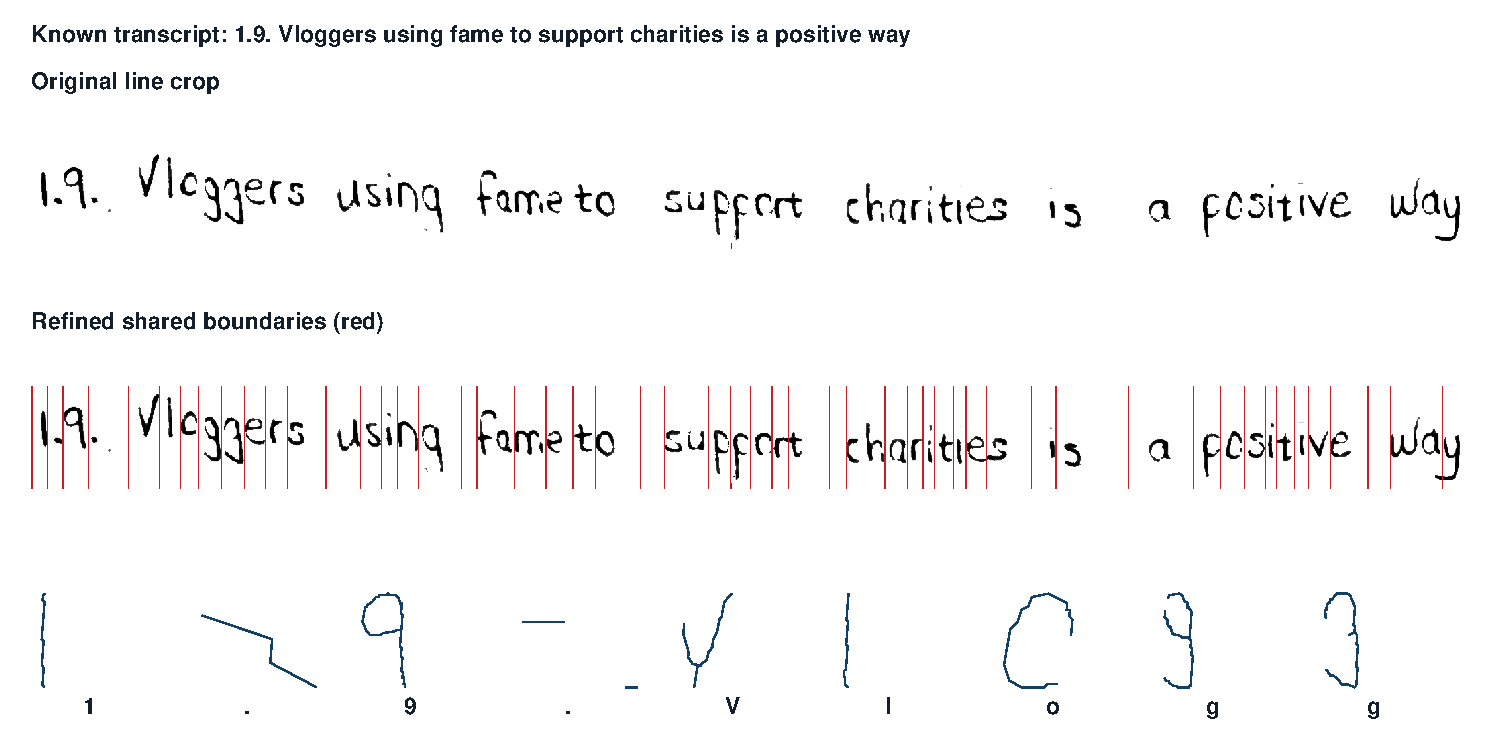
\includegraphics[width=0.96\linewidth]{Figures/design-glyph-alignment.pdf}
\caption{Transcript-constrained character localisation and refinement of glyph boundaries.}
\label{fig:des-alignment}
\end{figure}

\subsubsection{Skeleton tracing and pen path construction}
Ink is an area, whereas the gantry needs a path. Zhang--Suen thinning reduces the line mask to a one-pixel centreline~\cite[p.~237]{zhang1984}. The complete line is thinned before character cells are separated. Thinning each cut cell independently would introduce an artificial image edge at every character boundary and could change the recovered centreline there.

The skeleton is treated as a graph: adjacent ink pixels form edges, and endpoints and junctions determine where paths begin or split. Redundant diagonal edges are suppressed when an orthogonal route already connects the same local pixels. The default tracer first splits paths at junctions, prunes short dangling spurs, then greedily rejoins nearby ends with a continuation angle below $75^\circ$. Thus the default is not simply one pen lift per junction. A separate through-junction tracer exists but is not enabled by default. Neither procedure establishes natural pen order: the image records final ink, and several stroke sequences can create the same graph.

Traced paths are divided at the character boundaries and simplified while limiting geometric deviation, following the polyline-simplification principle of Douglas and Peucker~\cite{douglas1973}. Short spurs and cut ligature tails require care because a genuine small stroke can resemble a skeleton artefact. Isolated dots may thin to a single point with no traceable edge; these are recovered as short paths rather than silently discarded.

A detached \texttt{t} or \texttt{f} crossbar can extend over the next character cell. The extractor checks its width, flatness and height and, when the configured crossbar rule applies, assigns the complete bar to the corresponding letter instead of splitting it at a vertical cut. Such an overlap is not recorded as an in-word pen connection. Without this distinction, a crossbar would both contaminate the next glyph and inflate the profile's connectedness.

The project uses the following coordinate transform to separate source-image size, baseline and slant from the geometry to be stored. Slant normalisation uses the shear principle described for cursive writing~\cite{vinciarelli2001}; the following coordinate convention is defined for this project. Equation~\ref{eq:des-glyphcoords} first expresses each path point relative to the cut boundary $x_L$ and baseline $b$, using the estimated x-height $h_x$ and slant $\phi$.
\begin{equation}
v=\frac{b-y}{h_x},\qquad
u_0=\frac{x-x_L}{h_x}-v\tan\phi,\qquad u=u_0-\delta.
\label{eq:des-glyphcoords}
\end{equation}
A traced point on this \texttt{V} is $(x,y)=(173,59)$, with left cut $x_L=146$, baseline $b=107$, $h_x=38$ and $\tan\phi=-0.0787017$. Equation~\ref{eq:des-glyphcoords} gives $v=48/38=1.263158$ and $u_0=27/38-1.263158(-0.0787017)=0.809939$. After the implementation's three-decimal intermediate rounding and measured post-trim shift $\delta=0.4472489$, the stored point is $(u,v)=(0.363,1.263)$ and the recorded lead is 0.447 x-heights.

Image rows increasing downwards become glyph height increasing upwards. After trimming eligible ligature tails, the code sets $\delta=\min(u_0+v\tan\phi)$ over the remaining points, subtracts it from the stored horizontal coordinates and records lead $l=\operatorname{clip}(\delta,0,1.5)$. Thus the stored path and its lead are separate quantities: they preserve the relation between the character cell and the ink rather than forcing every cell to start at its first stroke. Slant is removed for storage and reapplied during placement. The glyph can then be drawn at a chosen physical x-height instead of a fixed number of source pixels.

Entry and exit positions are recorded along with whether the skeleton crosses a character boundary. This distinguishes a measured original connection from a merely small visual gap. The extracted paths still represent a geometric reconstruction, rather than the writer's true pen trajectory: retracing, pressure and movement direction cannot generally be recovered uniquely from a static image.

Figure~\ref{fig:vt-tracing} follows a real Owen line fragment from ink area to centreline and then to simplified paths. Across the complete traced line, 85 paths contain 3\,738 vertices before simplification and 974 afterwards, using the extraction tolerance of 0.6 source pixels. This removes 2\,764 vertices, approximately 74\%, before later glyph placement. Path colours and start markers also expose the separate pen strokes. The order is inferred from static ink and does not recover the writer's original stroke timing. Appendix~\ref{app:vt-glyphgeometry} connects the resulting points to the stored glyph frame and connectedness count.

\begin{figure}[!htbp]\centering
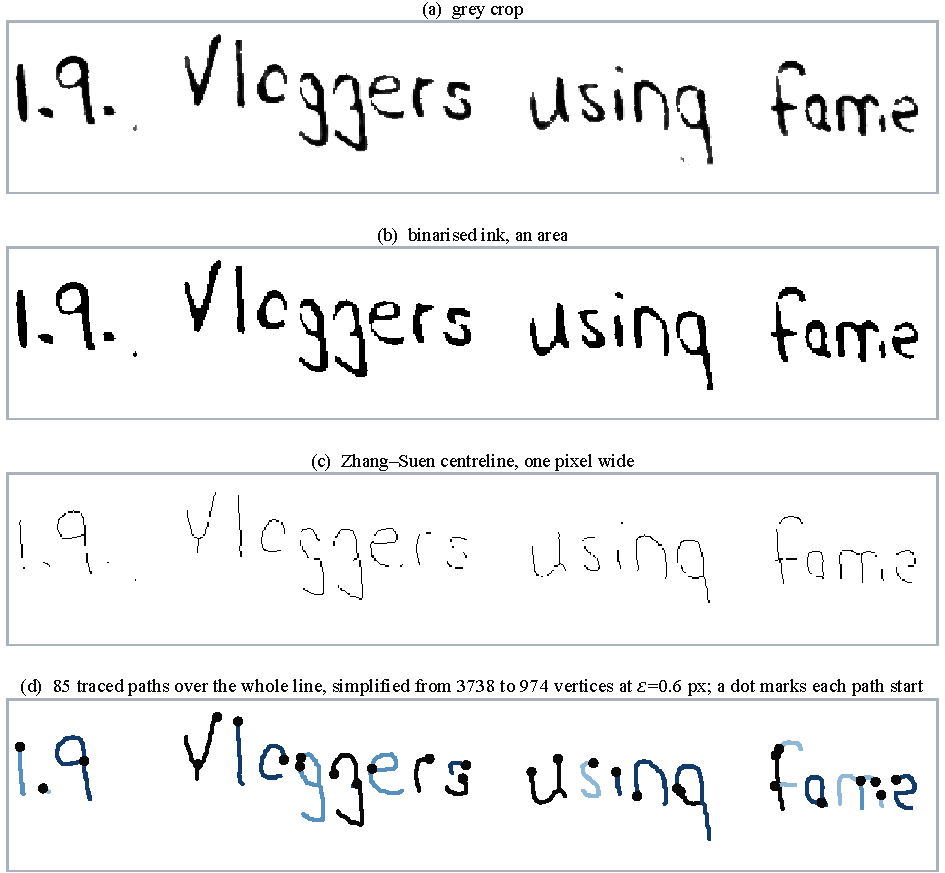
\includegraphics[width=\linewidth]{Figures/VisualTests/T41_skeleton_trace_simplify.pdf}
\caption{Real ink, its thinned centreline and the traced paths after bounded simplification.}
\label{fig:vt-tracing}
\end{figure}

\subsubsection{Glyph selection and library quality}
The library must retain variation without giving every cut equal credibility. A recogniser can assign the correct transcript while placing one boundary inside a letter, so alignment is followed by geometric and consistency checks. Low-confidence lines are filtered relative to the writer's own alignment distribution. Per-glyph checks reject implausible width, height, stroke count, pen length and disagreement between ink width and the allocated character advance.

The width gate allows up to 2.1 x-heights for ordinary characters and 2.9 for wide characters such as \texttt{m} and \texttt{w}. Further width and height checks use the character's own distribution, rather than applying one absolute size to every letter. The 40th-percentile width provides a reference less easily enlarged by a few cuts that contain part of a neighbour. Tightening is retained only when enough variants survive to form a usable pool. These gates encode plausible glyph geometry; their exact values are engineering heuristics, not universal typographic laws.

A cross-writer shape prior supplies a second check. Each variant is represented by a smoothed, normalised $12\times12$ occupancy descriptor. Pooling descriptors of the same character across writers gives a robust reference shape. Its role is to reject malformed cuts from a writer's own library, not to copy another writer's letter into it. Internal consensus then favours variants close to the writer's typical form. The ordinary variant pool is limited to twelve per character; an accepted denoised prototype can be prepended as an additional candidate.

For unit-length descriptor $v_g$ and the normalised median reference $r_c$ for character $c$, the prior distance is $d(g,c)=1-v_g^Tr_c$. Internal consensus instead uses pairwise $L_1$ descriptor distances and chooses the medoid with the lowest total distance. These compare a pooled character reference with this writer's own forms. Dylan's first stored \texttt{a} variant has recorded prior distance 0.114. Recomputing the pairwise rule on all nine final stored variants gives the smallest total distance, 33.3413, for variant index 4; the other totals range from 34.4306 to 42.9091. This demonstrates the selection rule on the final pool, without treating a new descriptor calculation as the historical filtering log. Algorithm~\ref{alg:des-profile} gives its place in profile construction.

\begin{designalgorithm}
\caption{Labelled handwriting to a persistent writer profile}
\label{alg:des-profile}
\prequire{Labelled original lines $\mathcal L$, trained reader and writer identifier.}
\begin{designpseudo}
\pstate{0}{$\mathcal G\leftarrow\varnothing$; $\mathcal S\leftarrow\varnothing$}
\pstate{0}{\textbf{for each} $(G,\ell)\in\mathcal L$ \textbf{do}}
\pstate{1}{$A\leftarrow\operatorname{ForcedAlign}(G,\ell)$; estimate baseline, x-height and slant}
\pstate{1}{\textbf{if} alignment or body band is unusable \textbf{then continue}}
\pstate{1}{Refine shared increasing cuts; thin full line; trace skeleton paths}
\pstate{1}{Split paths at cuts; assign crossbars; recover untraced dots}
\pstate{1}{Normalise glyph coordinates; record advance, lead and boundary crossings}
\pstate{1}{Append glyphs to $\mathcal G$ and line measurements to $\mathcal S$}
\pstate{0}{\textbf{end for}}
\pstate{0}{Cache raw extraction; reject low-confidence lines relative to this writer}
\pstate{0}{\textbf{for each} character's glyph pool $\mathcal G_c$ \textbf{do}}
\pstate{1}{Apply size, height-class, path-length and cell-consistency gates}
\pstate{1}{Refine size range; apply cross-writer prior and within-writer consensus}
\pstate{1}{Rank and smooth retained variants; construct medoid and eligible prototype}
\pstate{0}{\textbf{end for}}
\pstate{0}{\textbf{return} persistent profile containing $\mathcal G$ and robust summaries of $\mathcal S$}
\end{designpseudo}
\end{designalgorithm}

Two additional representatives support stable generation: a medoid that is an actual extracted example, and a denoised prototype formed from compatible variants. Prototype strokes are aligned and resampled before taking robust summaries; different stroke counts are not averaged indiscriminately. A prototype is admitted as an additional candidate only when the implemented shape-prior test improves sufficiently. The filtering distinguishes handwriting variation from implausible extraction geometry.

Synthesis preferentially samples well-formed variants and can favour a compatible entry height when joining. Where the requested character is unavailable, the code can use a case-related shape, a similar form, an anchor glyph or a simple fallback. These options preserve the ability to generate text, but they do not establish that the missing character was reproduced in the writer's own style. The trajectory records glyph-source information so that fallback use can be distinguished from genuine extracted forms.

The final stored profiles supply the glyph geometry used during the demonstration. Figure~\ref{fig:des-profile-example} compares the final nine-variant \texttt{a} pools for Owen, Dylan and Yeukita alongside their representative forms. These paths can be inspected independently of a photograph or a generated sentence, making it possible to distinguish the stored shape from later slant, jitter and connector operations.

\begin{figure}[!htbp]\centering
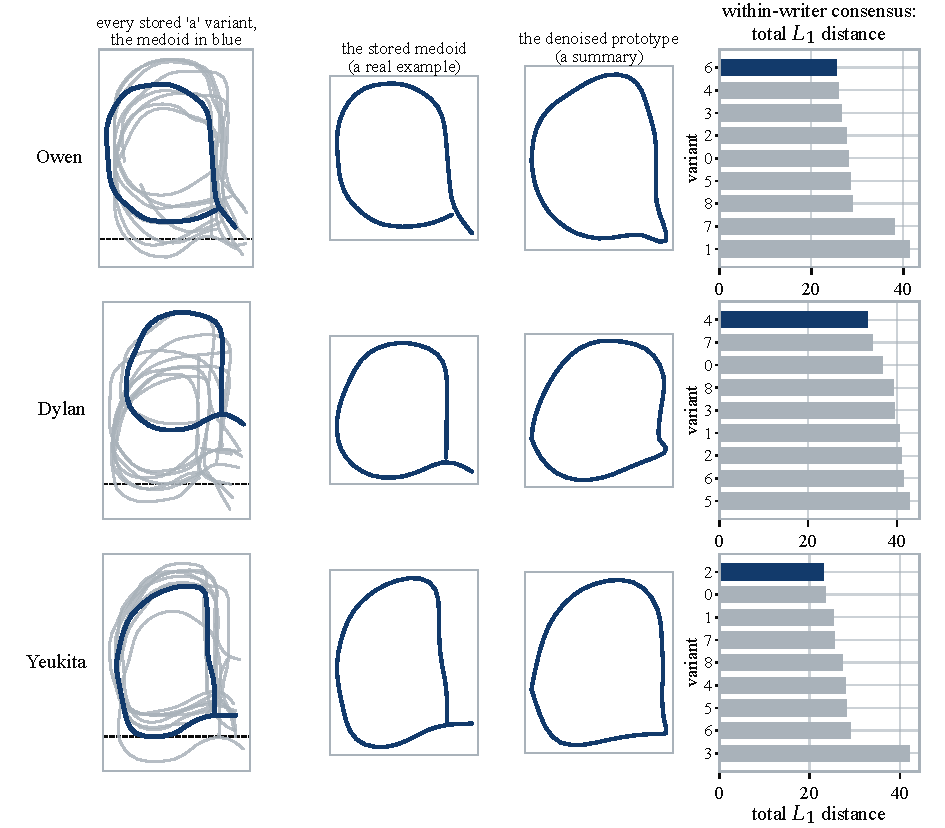
\includegraphics[width=\linewidth]{Figures/VisualTests/T45_variant_pool_medoid.pdf}
\caption{Variant clouds, actual medoids, denoised prototypes and within-writer distance totals for three final profiles.}
\label{fig:des-profile-example}
\end{figure}

Each displayed \texttt{a} pool contains nine variants. Their overlaid paths retain recognisable loop geometry while differing in closure and curvature; the distance bars show why a particular real example is selected. The medoid and median prototype remain distinct: one selects a real variant, while the other combines compatible paths. A low prior distance expresses resemblance to the character reference, not proof of a better match to the writer.

\subsubsection{Writer style measurement and storage}
\label{sec:des-profile}
Letter shapes alone do not determine the appearance of a line. The profile also stores slant, x-height, ascender and descender extent, word spacing, per-character advance and connectedness. Measurements use medians where a few unusual cuts could otherwise dominate the result. Table~\ref{tab:des-styleparameters} in Appendix~\ref{app:des-reference-tables} gives the stored quantities, their units and their use in synthesis.

Slant is estimated by shearing the ink through candidate angles and measuring concentration of the resulting column profile. The stored angle is the one that most nearly aligns the dominant strokes. This treats slant as a property measured over a line, so it is less dependent on one unusual letter. It remains an estimate affected by letter content; it is not a direct observation of the writer's hand motion.

Building on the use of textural and shape features for writer characterisation~\cite[p.~701]{bulacu2007}, this project defines connectedness as the fraction of eligible adjacent non-space glyph boundaries crossed by a source skeleton, as shown in Equation~\ref{eq:des-connectedness}.
\begin{equation}
c=\frac{N_{\mathrm{cross}}}{\max(1,N_{\mathrm{adj}})}.
\label{eq:des-connectedness}
\end{equation}
For the single extracted Owen line used above, 39 eligible adjacent non-space glyph pairs were counted and three boundaries were crossed by a recovered skeleton. Equation~\ref{eq:des-connectedness} gives $c=3/39=0.076923$. This line-level extraction trace illustrates what is counted; the final stored writer profile summarises its own complete source collection.

Here $N_{\mathrm{adj}}$ counts eligible adjacent non-space glyph pairs and $N_{\mathrm{cross}}$ counts boundaries actually crossed by a traced centreline. Equation~\ref{eq:des-connectedness} measures connections in the source writing; counting pen lifts in a generated file would instead measure the extractor and synthesiser's decisions. The difference is important when assessing how faithfully the library represents cursive writing.

Profiles are stored as structured files containing the writer identifier, measurements and glyph paths. The permanent representation supports the proposal's multiple-writer requirement without re-extracting the source pages for each request. Cached raw extraction also permits a change to filtering without repeating all tracing. The extraction cache and final profile have different purposes: the former preserves intermediate work, while the latter is the version selected for reproduction.

\subsubsection{Text layout and connected handwriting synthesis}
\label{sec:des-layout}
The synthesiser receives digital text, a profile, a physical x-height and a line-width limit. It selects a variant for each character, applies controlled shape variation and places the resulting paths into words and lines. Character advance and word spacing are taken from the profile rather than placing every letter at a fixed cell width. A word is moved to the next line when its predicted width exceeds the remaining space.

Equation~\ref{eq:des-placement} is the project's inverse placement transform: it reapplies slant and physical scale to the stored glyph coordinates before machine-coordinate conversion.
\begin{equation}
x=p_x+h_x^{\mathrm{mm}}(l+u+sv),\qquad
y=p_y+h_x^{\mathrm{mm}}(v+d).
\label{eq:des-placement}
\end{equation}
In the generated Owen sentence ``Writing with style.'', the first placement call, after calibration and jitter, uses $(u,v)=(-0.01134565,1.47270173)$, lead $l=0.25117988$, zero shear and drift, and $h_x^{\rm mm}=4$. With the initial placement origin $(0,0)$, Equation~\ref{eq:des-placement} gives $x=4(0.25117988-0.01134565)=0.9593369$\,mm and $y=4(1.47270173)=5.8908069$\,mm. This is the actual assembly point before later path processing and machine placement, not a replay of the earlier \texttt{V} crop.

Here $(u,v)$ is a stored glyph point, $l$ is its lead-in offset, $s$ is the applied slant shear, $d$ is local baseline drift, and $(p_x,p_y)$ is the placement origin. The physical x-height $h_x^{\mathrm{mm}}$ converts the normalised path to millimetres. Equation~\ref{eq:des-placement} keeps the source shape, line layout and physical scale as separate quantities.

Small random translations, rotations and scale changes avoid using identical paths for every occurrence of a letter. A correlated drift term changes the baseline gradually instead of introducing unrelated vertical jumps. The implemented drift update uses a persistence factor of 0.85 and bounds displacement to $\pm0.25$ x-heights. Such variation is controlled rather than unrestricted: too much jitter degrades letter identity and can cause neighbouring glyphs to collide. A collision guard maintains a nominal 0.05 x-height clearance where appropriate.

Variant choice is weighted rather than uniform: the best-ranked forms receive greater probability, and a compatible entry height is preferred when joining. The legibility anchoring strength is also profile-dependent. In the automatic setting, Equation~\ref{eq:des-anchor} maps the median stored prior distance $\widetilde d$ into a value $\lambda$.
\begin{equation}
\lambda=\operatorname{clip}\left(\frac{\widetilde d-0.24}{0.32-0.24},0,1\right).
\label{eq:des-anchor}
\end{equation}
The final Owen profile's stored glyph distances have median $\widetilde d=0.18355$. Equation~\ref{eq:des-anchor} gives $\lambda=\operatorname{clip}[(0.18355-0.24)/0.08,0,1]=0$. With no stored override, this is the anchoring value selected by the automatic rule for the generated job.

A clean library therefore retains more sampled personal variants; a library with poor descriptor agreement uses stronger anchors. The anchor first prefers an acceptable representative from the writer's own profile, then uses a generic form when necessary. Equation~\ref{eq:des-anchor} is a heuristic for allocation of trust, not a learned probability that a glyph is correct. Source tags identify own, case-related, similar, core, fallback or blank output. In particular, ``core'' can represent either a personal representative or a generic anchor; that tag alone cannot quantify how much personal geometry was preserved.

For connected writing, the profile's connection fraction is used as a probability for eligible neighbouring letters. The code suppresses joining for profiles below a 0.45 connection threshold. A proposed join also requires a compatible glyph source and a gap no greater than 0.80 x-heights. This prevents a generic print fallback from being treated as a natural cursive attachment and prevents a long flat connector across an unusually large space. The body stroke is distinguished from a dot or crossbar so that the next letter does not connect to a detached mark.

The default connector uses a shallow curved path between the exit and entry points, with sag limited relative to x-height and separation. A tangent-based alternative exists, but its flag is disabled in the current configuration. When a join is accepted, the connector and both bodies form one continuous pen-down path.

Line-level style calibration compensates for differences between measurements of individual stored glyphs and measurements of the assembled line. A probe is rendered without jitter, measured using the same style functions, and compared with the reference slant and vertical proportions. Limited shear and extent corrections are applied over three iterations. This improves internal consistency of the representation, but it remains calibration against the project's own measurements; independent evaluation is needed to establish physical stylistic fidelity.

\subsubsection{Candidate selection for legibility and writer identity}
\label{sec:des-selection}
One set of random variant choices can be more readable than another without being more characteristic of the writer. Candidate selection therefore evaluates both quantities. Each candidate trajectory is rendered at constant ink width, read by the text recogniser, and judged by the stroke-normalised writer classifier introduced in Section~\ref{sec:des-shapenamer}. Uniform rendering keeps candidate selection focused on reproducible geometry, while the shape classifier applies the selected stroke-normalisation convention.

The project-defined score in Equation~\ref{eq:des-jointscore} combines text recovery and the requested writer's probability. It uses the insertion, deletion and substitution error convention of Graves et al.~\cite[p.~2]{graves2006}, then combines the resulting character score with the writer posterior using a harmonic mean.
\begin{equation}
A=\max\left(0,1-\frac{d_{\mathrm{edit}}(\widehat t,t)}{|t|}\right),\qquad
J=\begin{cases}2AP/(A+P),&A+P>0,\\0,&\text{otherwise}.\end{cases}
\label{eq:des-jointscore}
\end{equation}
For the recorded Owen candidate 1, the 19-character target ``Writing with style.'' differs from its reader output by one substitution, giving $A=18/19=0.9473684$. The selected-writer posterior is $P=0.5786133$, so Equation~\ref{eq:des-jointscore} gives $J=0.7184359$. This is the actual score used to select the candidate in Figure~\ref{fig:des-candidates}; it evaluates the software rendering rather than physical stylistic agreement.

Here $t$ is intended text, $\widehat t$ is recognised text, $d_{\mathrm{edit}}$ is the minimum number of insertions, deletions and substitutions, using the reader error convention~\cite[p.~2]{graves2006}, and $P$ is the model probability of the selected writer. The harmonic mean $J$ in Equation~\ref{eq:des-jointscore} makes a weak component limit the combined score. The actual candidate comparison below holds text and writer fixed, showing how the writer posterior affects selection.

Algorithm~\ref{alg:des-joint} gives the bounded search and repair procedure. The server default is fourteen candidates, with the number configurable. Because an entire candidate is rerendered and rescored, a repair is judged in its assembled context rather than by an isolated character score.

\begin{designalgorithm}
\caption{Joint candidate search and bounded legibility repair}
\label{alg:des-joint}
\prequire{Text, writer profile, reader, shape classifier, seed $s$ and trial budget $K$.}
\begin{designpseudo}
\pstate{0}{$J^*\leftarrow-1$; $R\leftarrow\varnothing$; determine anchoring strength}
\pstate{0}{\textbf{for} $k\leftarrow0$ \textbf{to} $\max(1,K)-1$ \textbf{do}}
\pstate{1}{$T\leftarrow\operatorname{SynthesizeText}(\text{text},\text{profile},s+977k)$}
\pstate{1}{$I\leftarrow\operatorname{RenderUniformInk}(T)$; $(A,P,J)\leftarrow\operatorname{Score}(I)$}
\pstate{1}{\textbf{if} $J>J^*$ \textbf{then} $(T^*,I^*,J^*)\leftarrow(T,I,J)$}
\pstate{1}{\textbf{if} $J^*\geq0.99$ \textbf{then break}}
\pstate{0}{\textbf{end for}}
\pstate{0}{\textbf{for} at most three configured repair rounds \textbf{do}}
\pstate{1}{\textbf{if} $J^*\geq0.995$ \textbf{then break}}
\pstate{1}{$W\leftarrow$ up to two weak aligned positions not already in $R$}
\pstate{1}{\textbf{if} $W=\varnothing$ \textbf{then break}}
\pstate{1}{$R'\leftarrow R\cup W$; regenerate with stronger anchors at $R'$ and seed $s$}
\pstate{1}{Render and rescore the complete trial trajectory}
\pstate{1}{\textbf{if} $J>J^*$ \textbf{then} commit $R'$ and the new best trajectory}
\pstate{0}{\textbf{end for}}
\pstate{0}{\textbf{return} $T^*$ with selection and accepted-repair metadata}
\end{designpseudo}
\end{designalgorithm}

A repair is retained only when the complete trial improves the joint score. This bounds the search and protects the best candidate already found. A separate reader-only helper uses a different escalation policy; it is not part of this joint selection procedure.

More trials increase the opportunities to find a useful combination, but also add recogniser and writer-model calls. Search quality therefore has a computational cost for fixed text and profiles. The repaired or fallback glyph proportion also matters: legibility gained by replacing distinctive forms has a stylistic cost. Figure~\ref{fig:des-candidates} relates the individual candidate scores to the selected trajectory.

\begin{figure}[!htbp]\centering
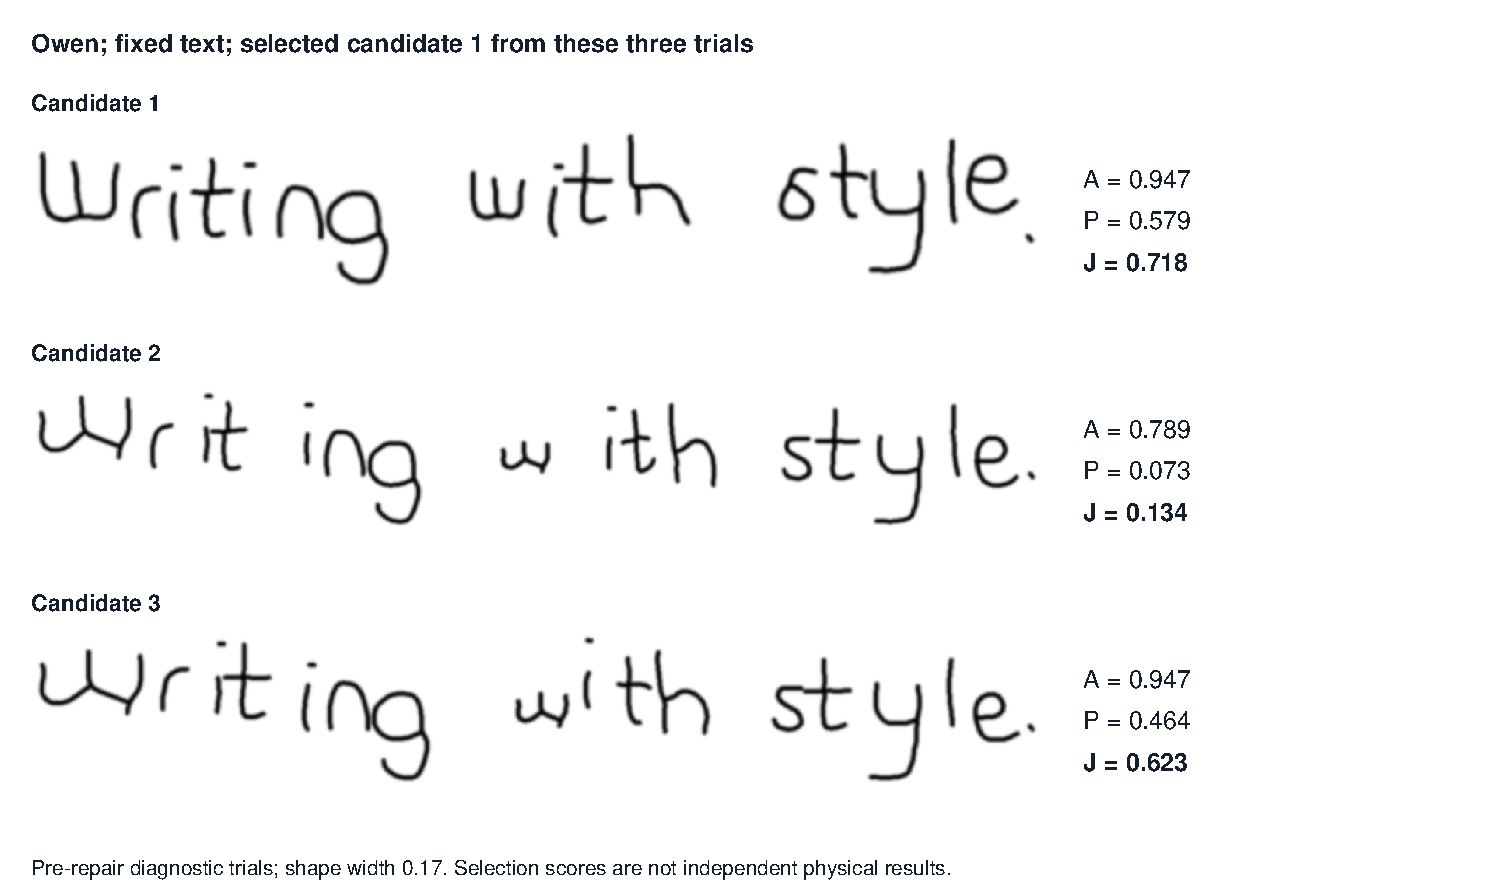
\includegraphics[width=0.95\linewidth]{Figures/design-candidate-selection.pdf}
\caption{Example of joint candidate selection for a fixed writer, input text and search configuration.}
\label{fig:des-candidates}
\end{figure}

In the worked Owen example, three pre-repair trials use the fixed text ``Writing with style.'', seeds 2026, 3003 and 3980, and the selected eleven-writer shape model with an explicit width fraction of 0.17. Candidate 1 has $(A,P,J)=(0.947,0.579,0.718)$, while candidate 3 has the same character score but $(P,J)=(0.464,0.623)$. The combined criterion therefore selects candidate 1. Its reader output begins with a lower-case ``w'', which accounts for one edit rather than perfect text recovery. This is an inspectable scoring example before repair, not a claim that the full default search or the physical system attained those scores.

The same models guide selection, so their scores cannot independently prove the output's quality. A classifier can prefer an image for model-specific reasons, and its posterior is not an 85\% stylistic correlation measurement. The search is a design mechanism; final physical handwriting must be qualified separately. Increasing the search budget also does not recover a letterform that is absent or incorrectly extracted from the source library.

\subsubsection{Machine coordinate mapping and G-code generation}
\label{sec:des-gcode}
The selected trajectory is mapped into the calibrated workspace. Normalised glyph size, line spacing and machine margins are handled separately: fitting the height of a tall descender should not silently change the meaning of the ruling or move a line outside the available area. Robust extent measurements limit the effect of a single unusually tall glyph on the scale of the complete passage.

The physical x-height is first chosen from the page ruling and a stored x-height-to-pitch ratio where available. If that ratio is absent, the configured fallback gives $8.4(0.46)=3.864$\,mm at the default 8.4\,mm ruling. This is the fallback sizing rule, rather than the value passed to every job: the traced Owen job explicitly requests 4\,mm. A probe of the requested text can reduce the selected value if robust line extent exceeds 1.25 rulings. The extent uses the 98th-percentile stroke tops and second-percentile bottoms, with exact extremes for fewer than eight strokes. It limits outliers but does not guarantee every extreme lies inside the nominal band.

Two placement modes are supported. Ruled placement adjusts each line's measured centre to the configured ruling independently of the character scale. Free placement preserves the synthesised pitch after scaling, which can avoid forcing large ascenders and descenders from neighbouring lines into contact. A line offset selects a later starting position and reduces the remaining page height. The full conversion procedure is retained as Algorithm~\ref{alg:des-machine} in Appendix~\ref{app:des-machine-procedure}.

For the basic mapping, Equation~\ref{eq:des-machinecoords} places a trajectory with bounds $(x_0,y_0,x_1,y_1)$ within the page margins.
\begin{equation}
x_m=o_x+m_x+a(x-x_0),\qquad
y_m=o_y-m_y-d_y-a(y_1-y)+\Delta_y.
\label{eq:des-machinecoords}
\end{equation}
The generated Owen trajectory has $x_0=0.9593369$\,mm and $y_1=6.6340616$\,mm. A point $(2.9829210,5.3303251)$\,mm is placed using the configured origin $(0,251.3)$\,mm, margins $(15,10)$\,mm, unit fit scale and zero line shift. Equation~\ref{eq:des-machinecoords} gives $(x_m,y_m)=(17.0235840,239.9962635)$\,mm. Three-decimal file emission writes this point as \texttt{X17.024 Y239.996}, connecting the trajectory calculation to the motion segment examined in Section~\ref{sec:des-drive}.

Here $(o_x,o_y)$ is the configured machine origin, $m_x,m_y$ are margins, $a$ is a fit scale, $d_y$ selects the line offset and $\Delta_y$ is any line-spacing adjustment. Both stored trajectories and machine coordinates use upward-increasing $y$; Equation~\ref{eq:des-machinecoords} positions later lines lower on the page rather than introducing another arbitrary image flip. Requested points are restricted to the usable travel, but clamping is a last boundary protection: it can distort a letter and must not be treated as successful layout.

Strokes are ordered within text rows so that path shortening does not scramble reading order. Short path segments can be decimated, and nearby consecutive strokes may be joined without a lift. The current default distance is 0.6\,mm for such joins and for closing a near-complete ring. These operations save travel and pen changes, but can also introduce unintended ink if set too aggressively; their scale relative to the chosen writing size matters. The code retains clipped-point and stroke information to make these effects inspectable.

The generated file selects millimetres and absolute positioning. A travel move reaches the start of a stroke with the pen raised, the pen is lowered, drawing moves follow, and the pen is raised before the next travel. Figure~\ref{fig:des-gcode-excerpt} reproduces the beginning of the actual generated Owen file used for these calculations. The interpreter assigns \texttt{M3} and \texttt{M5} to pen down and pen up respectively.

\begin{figure}[!htbp]
\begin{lstlisting}[style=designcode]
G21
G90
G0 F2400
G0 F2400 X15.000 Y240.557
M3
G4 P0.350
G1 F900
G1 X15.001 Y240.207
G1 X15.002 Y239.857
G1 X15.003 Y239.506
G1 X15.005 Y239.156
G1 X15.006 Y238.806
G1 X15.007 Y238.456
\end{lstlisting}
\caption{Opening commands of the generated Owen sentence, including its actual travel/drawing feeds and first drawing coordinates. The file was inspected offline and not executed on the gantry.}
\label{fig:des-gcode-excerpt}
\end{figure}

Feed is modal, so the travel feed is restated after drawing rather than assuming that the first \texttt{G0 F} remains active. Pen dwell defaults to 350\,ms in each direction and is configurable separately for raising and lowering. This dwell is additional to the switch-confirmed actuation performed by the interpreter. A timing estimate that counted only geometric travel would omit those repeated state-change costs. Conversely, a trapezoidal acceleration parameter in a configuration object does not establish that the actual GPIO loop executes acceleration ramps.

Equation~\ref{eq:des-timebudget} is a dimensional calculation of the nominal job budget: distance divided by feed gives travel time, and pen-state changes add their configured dwells.
\begin{equation}
t_{\mathrm{nom}}=\frac{60D_d}{F_d}+\frac{60D_u}{F_u}
+\frac{N_p(t_{\mathrm{up}}+t_{\mathrm{down}})}{2}.
\label{eq:des-timebudget}
\end{equation}
For this same generated file, the unrounded distance accumulators are $D_d=139.0263729$\,mm and $D_u=158.1555743$\,mm. At $F_d=900$ and $F_u=2400$\,mm/min, with 56 pen transitions and two 0.35\,s dwell settings, Equation~\ref{eq:des-timebudget} gives $t_{\rm nom}=9.2684249+3.9538894+19.6=32.8223142$\,s. The job metadata reports 32.8\,s after rounding. This is the converter's actual geometric budget, not a physical completion-time measurement.

Here $D_d,D_u$ are drawing and pen-up distances in millimetres, $F_d,F_u$ their feeds in mm/min, $N_p$ is the number of pen transitions and the dwell times are in seconds. The last term assumes alternating up/down events. Equation~\ref{eq:des-timebudget} separates settings that affect ink quality from settings that mainly affect non-writing time. It excludes the unknown initial approach to the first stroke, synthesis, switch-confirmed motor actuation, GPIO overhead and the directional pulse-delay effect in Equation~\ref{eq:des-pulsetime}; the saved estimate is therefore not the measured R3 completion time.

Figure~\ref{fig:vt-timeparts} applies the same budget calculation to a separate offline generation of ``Writing with style.'' in four final profiles. The Owen job contains 58 pen transitions: its recorded components are 9.249\,s drawing, 3.198\,s travel and $58(0.35)=20.3$\,s dwell, giving 32.747\,s in total. Thus dwell contributes about 62\% of this nominal budget; across the four jobs it contributes between 52.7\% and 65.1\%, the lowest share belonging to Abhinav, whose larger hand spends 15.971\,s drawing. The different path and transition counts distinguish these jobs from the earlier worked file. The breakdown identifies a drawing-side optimisation opportunity, but shortening dwell would require a physical test that the pen still clears and settles reliably. These estimates exclude the execution costs stated above and are not additional R3 timing measurements.

\begin{figure}[!htbp]\centering
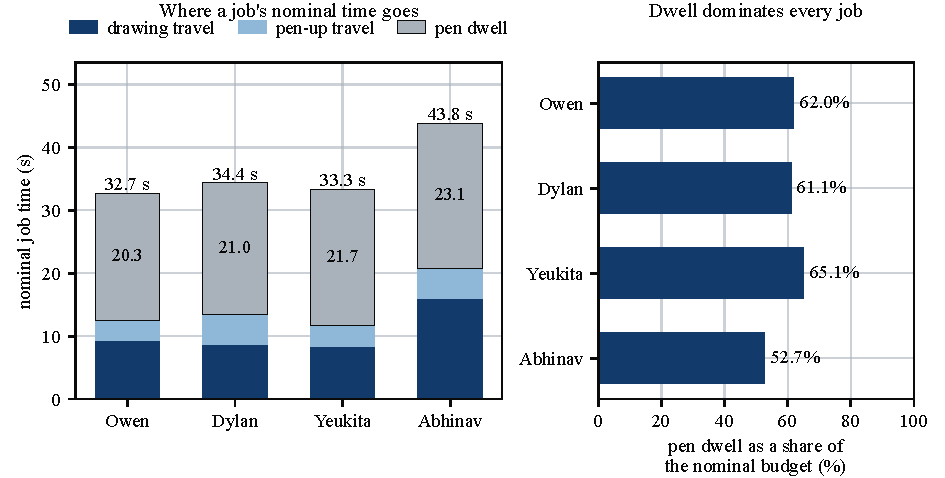
\includegraphics[width=\linewidth]{Figures/VisualTests/T56_time_budget.pdf}
\caption{Nominal drawing, travel and dwell budgets for the same sentence generated from the Owen, Dylan, Yeukita and Abhinav profiles.}
\label{fig:vt-timeparts}
\end{figure}

\subsubsection{Reproduction verification and design limitations}
The reproduction checks follow the representations established above: aligned source ink, stored glyph paths, assembled trajectories and emitted machine commands. Re-rendering the emitted G-code can reveal a coordinate inversion, scale change, missing stroke or additional joining segment before drawing. Comparing that render with the selected trajectory checks conversion; comparing the physical drawing with the render checks execution. These comparisons localise errors without substituting for end-to-end qualification.

Appendix~\ref{app:des-visual-tests} shows the same sentence generated from four stored profiles alongside paths independently parsed from their emitted G-code. Nine controlled conversion fixtures additionally preserved path vertex counts with no clipping and a maximum coordinate discrepancy of $0.0004$\,mm, consistent with writing coordinates to three decimal places. Joins and ring closure were disabled only for those correspondence fixtures so that the vertices could be paired; the four profile illustrations used the normal configuration. Neither check measures the mechanism's positional accuracy.

The representation's main advantage is that its geometry is explicit and inspectable. A defective glyph can be traced to a source crop, stored paths can be viewed independently of the machine, and physical size follows from a defined transformation. The main limitation is the loss of context when a connected word is divided into reusable characters. Real letterforms change with their neighbours, whereas a finite glyph pool and join rules approximate that dependence. Skeletons also omit pressure and true temporal order. These losses explain why a plausible letter library need not reproduce every connected style equally well.

Possible extensions include context-dependent multi-character units, better alignment, trajectory acquisition and a verified alternative junction tracer. Each addresses a different loss: multi-character units preserve local letter interactions, trajectory acquisition restores temporal information, and improved tracing changes how an existing skeleton becomes strokes. Their implementation would require corresponding changes to extraction, storage or the source data, rather than a larger candidate search alone.
The retained design therefore prioritises extraction from the available offline pages and explicit control of the plotted geometry. Recovering natural pen dynamics would require new trajectory data, while replacing the library with a learned generator would add a separate training and validation problem. The alternative tracer remains an implementation option; its presence alone does not establish an improvement over the default.
\FloatBarrier

\subsection{System integration and embedded operation}
\label{sec:des-integration}
The server connects the numerical processing, models, profiles and motion interpreter. The browser supplies images or writing requests and displays their outputs; the engineering operations remain in the processing modules.

\subsubsection{Classification and reproduction workflows}
Captured and uploaded pages follow the same conditioning and recognition path. Writer predictions are combined across the retained line crops using Equation~\ref{eq:des-pagevote}, rather than choosing one line to represent the page.
\begin{equation}
\overline p_k=\frac{\sum_i w_i p_{i,k}}{\sum_i w_i},\qquad
\widehat k=\arg\max_k\overline p_k.
\label{eq:des-pagevote}
\end{equation}
Applying this vote to the first two archived Owen01 crops gives ink weights 20204 and 21750, with Owen probabilities 0.9996674 and 0.9999279 from the selected 0.17-width model. Equation~\ref{eq:des-pagevote} gives $\overline p_{\rm Owen}=(20204\times0.9996674+21750\times0.9999279)/41954\simeq0.9998024$. This is a two-crop calculation trace, not the full-page evaluation reported in Results.

Here $w_i$ counts crop pixels below grey value 128; all-zero weights fall back to equal weighting. More ink therefore gives a line greater influence, including a possible dark artefact. Crop rejection precedes aggregation for this reason. The pooled probability and the fraction of individual lines agreeing with the selected writer are reported separately; neither establishes accuracy without a reference.

A reproduction request selects text, profile and drawing settings, then stores the trajectory, preview, G-code and metadata as one generated job. Characters absent from the profile use the fallbacks in Section~\ref{sec:des-layout}. Drawing is a separate action requiring connection and calibration, allowing inspection before execution. Table~\ref{tab:des-contracts} in Appendix~\ref{app:des-reference-tables} records each representation's inputs, outputs and coordinate conventions.

\subsubsection{Embedded execution, interfaces and job control}
The ODROID N2+ runs NumPy inference and motion control from stored arrays, without the training framework. Canvas size, line count and candidate count still determine its processing load. NumPy supplies array arithmetic; Flask handles requests; image libraries handle file I/O; OpenCV serves the camera interface; and \texttt{gpiod} exposes GPIO. Framework network operations belong to the separate training route. The complete source code is supplied separately from this report for the AMS submission.

During motion, the pulse loop checks an abort event and confirmed end stops. A separate request thread permits a stop while drawing is active. End-stop trips latch a fault; the recovery routines attempt switch retraction, pen raising and parking under their required preconditions. The stop request is a software path, not an independent motor-power disconnect. A pen-state timeout remains consequential because subsequent travel may mark the sheet.

The resulting job states distinguish generation, refused execution, completed execution and interruption/failure. Calibration establishes the coordinate reference in software, but missed steps can invalidate its correspondence with physical position. Neither a saved preview nor emitted pulse counts prove that the nib followed the intended path.

\subsubsection{Integration verification and remaining constraints}
Interface checks should confirm consistent upload/camera processing, checkpoint-to-profile writer mapping, bounded G-code and truthful interrupted-job status. Formal classification accuracy, drawing accuracy and timing against the proposal remain in Results.

The diagnostic retracing route provides a useful bypass: page conditioning and line separation are followed by thinning, tracing and ordinary machine conversion, omitting the reader, glyph library and synthesis. Comparing its G-code render with a drawing helps distinguish execution from synthesis errors. Comparing the drawing directly with the photograph still includes conditioning, skeletonisation, filtering and coordinate errors; it does not isolate mechanics alone.

Per-stage records separate acquisition, segmentation, inference, generation and execution time. Generation metadata is carried into the writing record so that a complete reproduction interval can be reconstructed. R3/R4 qualification must specify its start/end events and use the intended platform; Windows development timings cannot establish an ODROID requirement.
\FloatBarrier


\clearpage
\renewcommand{\eprthepartname}{Results}
\section{Results}
\label{sec:results}
The qualification tests follow the six requirements of the Project Proposal in order of importance. The physical reproduction, photographed-page analysis and embedded timing records are kept identifiable so that each result can be traced to the part of the system that produced it. Section~\ref{sec:discussion} interprets the engineering consequences; this section states the procedures and measurements.

\subsection{Summary of results achieved}
\label{sec:res-summary}
Table~\ref{tab:res-summary} compares the proposal's intended functions and numerical specifications with the available measurements. A result above a numerical target is distinguished from a complete qualification of the corresponding requirement.

\begin{table}[!htbp]\centering\small
\setlength{\tabcolsep}{5pt}
\begin{tabular}{p{0.32\linewidth}p{0.48\linewidth}p{0.12\linewidth}}\toprule
\textbf{Intended outcome} & \textbf{Actual outcome} & \textbf{Location}\\\midrule
\textbf{R1.} Reproduce any desired digital text in a trained writer's style, with at least 85\% character accuracy and 85\% stylistic correlation. & Fourteen physical pages, 184 labelled lines and 5\,471 reference characters give 84.41\% read-back character accuracy. Seven of eleven writers individually exceed 85\%. Writer identification is 86.41\% by line and all fourteen page pools are correctly attributed. A new geometric comparison of the physical output with 156 original lines gives shape correlation 0.697, below 0.85. The two pooled targets are not met; the writer breakdown identifies demonstrated stronger cases. & QT~1; Appendix~\ref{app:res-evidence}\\[5pt]
\textbf{R2.} Decode handwritten content and identify its writer from the training set with 95\% overall accuracy. & Writer identification reaches 153/156 lines, 98.08\%, and 11/11 writer pools. The selected joint reader reaches 94.06\% character accuracy on 1\,076 validation lines; the numerical comparison reader reaches 94.39\%. The writer point estimate exceeds 95\%; the selected reader is 0.94 percentage points below it. A joint text-and-writer success rate is not inferred from these different populations. & QT~2\\[5pt]
\textbf{R3.} Reproduce desired text in a trained style at no slower than 4~s per character. & \textbf{Met on the completion-confirmed timing records.} All 25 positive-character ODROID records with an explicit program-end marker satisfy their allowances. The worst is 166.61~s for 43 characters, or 3.875~s per character. & QT~3\\[5pt]
\bottomrule\end{tabular}
\caption{Summary of results achieved against the Project Proposal.}\label{tab:res-summary}
\end{table}

\begin{table}[!htbp]\ContinuedFloat\centering\small
\setlength{\tabcolsep}{5pt}
\begin{tabular}{p{0.32\linewidth}p{0.48\linewidth}p{0.12\linewidth}}\toprule
\textbf{Intended outcome} & \textbf{Actual outcome} & \textbf{Location}\\\midrule
\textbf{R4.} Decode the text and identify its writer within $2+0.025x$~s for $x$ handwritten characters. & Two recorded ODROID requests take 46.26~s and 55.49~s, against logged-count allowances of 14.50~s and 26.55~s. \textbf{Not met on these requests.} A separate development-host experiment measures a 2.76-fold network speed improvement using batched library inference. & QT~4\\[5pt]
\textbf{R5.} Draw character trajectories while maintaining absolute positional error no greater than 0.5~mm. & All seven measured square/triangle feature lengths differ from nominal by less than 0.5~mm; the largest difference is 0.37~mm. This supports the calibrated dimensional accuracy. Absolute point-position error and repeated-word overlay performance are not fully qualified by feature lengths alone. & QT~5\\[5pt]
\textbf{R6.} Train at least ten writing styles and permanently store their character trajectory mappings. & \textbf{Met in the evaluated stored set.} Eleven writer identities have stored profiles and glyph mappings and are represented in the evaluated classifier. All eleven are exercised by the physical-output and writer-identification measurements. & QT~6\\[5pt]
\textbf{FC1.} Operate in a well-lit laboratory or office at 400--1000~lux. & Indoor camera captures and robot-page photographs demonstrate operation under the recorded capture conditions. No calibrated illuminance series establishes the complete 400--1000~lux range. & Sec.~\ref{sec:res-conditions}\\[5pt]
\textbf{FC2.} Operate on a stable, level, vibration-free surface. & The physical outputs demonstrate operation in the fixed test arrangement. Surface level and vibration are not quantified, so the evidence applies to that arrangement. & Sec.~\ref{sec:res-conditions}\\
\bottomrule\end{tabular}
\caption{Summary of results achieved against the Project Proposal (continued).}
\end{table}
\FloatBarrier

\subsection{Qualification tests}
\label{sec:res-qtp}
\subsubsection{Test material, configuration and measurement definitions}
\label{sec:res-method}
The final evaluation uses six IAM writers (150, 152, 153, 384, 552 and 588) and five photographed contributors, denoted A, B, O, T and Y. These are the eleven writers introduced in Section~\ref{sec:des-class}. The robot drew fourteen pages because some writers' text occupies two pages. The pages contain a common paragraph, a pangram and, where available, text from the writer's source material. The analysis contains 184 lines with corresponding transcripts; the writer-model comparison additionally evaluates one unpaired crop and therefore contains 185 crops.

The physical pages were produced by the gantry under ODROID control. Accuracy was subsequently scored from saved images on the development host. The embedded timing measurements were extracted from the preserved ODROID server log. This arrangement allows large image sets to be analysed while retaining actual on-device evidence for the time specifications. Numerical equivalence across processors is not assumed to be a new hardware accuracy test.

The reproduction read-back uses the joint reader used in the Design examples. The separate reader evaluation compares that reader with the evaluated scratch reader; the selected joint reader supplies the 94.06\% system result and the scratch reader supplies a 94.39\% comparison result. Both share the architecture in Section~\ref{sec:des-class}. Writer identification uses the eleven-class stroke-normalised classifier at the selected width of 0.17. Appendix~\ref{app:res-evidence} identifies the files by their content hashes, so checkpoints with the same filename cannot be confused.

Character accuracy is computed from the summed Levenshtein edit distance rather than by averaging percentages of unequal-length lines. With reference transcript $t_i$, recognised transcript $\hat t_i$ and distance $d_{\rm edit}$, the scoring definition follows the character-error convention used in handwriting recognition~\cite[p.~2]{graves2006}:
\begin{equation}
A_c=100\left(1-\frac{\sum_i d_{\rm edit}(\hat t_i,t_i)}{\sum_i|t_i|}\right).
\label{eq:res-char}
\end{equation}
For the physical pages, Equation~\ref{eq:res-char} gives $100(1-853/5471)=84.4087\%$. The selected reader gives $100(1-2719/45747)=94.0564\%$, while the numerical reader gives $100(1-2567/45747)=94.3887\%$. Insertions, deletions and substitutions all contribute to the numerator; the score is therefore not a binomial count of independently correct characters.

Writer identification is the number of correctly classified lines divided by the number evaluated. Pooled writer decisions aggregate the evidence from a group of lines and are reported separately. The archive's word score counts matching words at equal positions, divided by reference words; it is called \emph{word match} here. A word insertion can shift later positions, so this score must not be interpreted as one minus word edit error rate.

The measurement tools save transcripts, reference lengths, edit counts and predictions before aggregation. The reviewed tables and figures are regenerated from these saved records. Statistical intervals on line classifications use Wilson score intervals~\cite[pp.~209--212]{wilson1927}; because lines from one writer share writing and capture conditions, these are descriptive line-level intervals. Resampling whole writer groups gives an additional sensitivity check for the physical character score. Neither procedure creates additional independent writers.

\reportqt{qt:r1}{Reproduction of digital text in a trained writer's style (R1)}
\resstep{Objectives of the test or experiment}
Determine whether the complete image-to-profile-to-gantry system produces legible new text in the selected stored style. Evaluate the proposal's character target and distinguish measured geometric style similarity from the supplementary ability to identify the writer of the output.

\resstep{Equipment used}
The Cartesian gantry, two A4988 axis drivers, pen-lift mechanism and ODROID N2+ described in Section~\ref{sec:des-hardware}; the IMX179 USB autofocus camera; the stored writer profiles; the joint reader and eleven-class writer model; and the development host for image scoring. The retained page images are $3264\times2448$ pixels. The camera model and signal wiring follow the Hardware section.

\resstep{Test setup and experimental parameters}
The paragraph, pangram and source-text blocks are designated A, B and C. Their different lengths and content are retained in the analysis. A separate transcript follows the actual line breaks of each reproduced page. The final stored glyph libraries supply the paths; the scoring experiment does not introduce a manual glyph-editing step. Greedy CTC decoding is used without a language model. Writer images are normalised to 0.17 before classification. The physical pages represent the recorded jobs; a common search budget or feed is not inferred for jobs whose settings were not retained.

\resstep{Steps followed in the test or experiment}
\begin{enumerate}\setlength{\itemsep}{1pt}
\item Generate a writing job for the required text and profile, execute it on the gantry and photograph the output.
\item Segment and orient each photograph, then pair every scored crop with its intended transcript line and block.
\item Record the reader output, character edits, reference lengths and writer prediction for each pair.
\item Aggregate counts by block and writer, then pool each physical page's writer evidence.
\item Compare the character score with 85\% and retain the separate style measurements with their own populations and definitions.
\end{enumerate}

\resstep{Results or measurements}
Table~\ref{tab:res-r1-blocks} gives the 184 paired lines by text block. Figure~\ref{fig:res-writers} exposes the variation across writers; the full values are in Table~\ref{tab:app-r1-writers}. Figure~\ref{fig:res-physical} provides examples of actual robot output alongside both strong and more difficult cases.
\begin{table}[!htbp]\centering\small
\begin{tabular}{lrrrr}\toprule
\textbf{Text block} & \textbf{Lines} & \textbf{Characters} & \textbf{Character / \%} & \textbf{Writer / \%}\\\midrule
A: paragraph & 119 & 4041 & 84.88 & 91.60\\
B: pangram & 21 & 463 & 78.40 & 76.19\\
C: source text & 44 & 967 & 85.32 & 77.27\\
All & 184 & 5471 & 84.41 & 86.41\\
\bottomrule\end{tabular}
\caption{Read-back character accuracy and writer identification on the photographed robot output. These are different measures; writer identification is supplementary to the correlation target.}\label{tab:res-r1-blocks}
\end{table}

\begin{figure}[!htbp]\centering
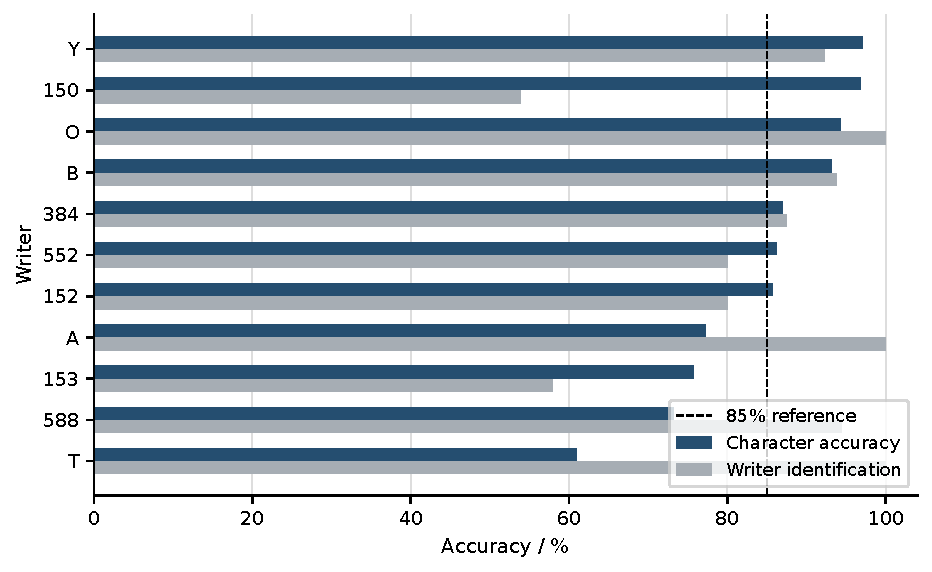
\includegraphics[width=0.98\linewidth]{Figures/results_writer_performance.pdf}
\caption{Physical reproduction by writer. Character accuracy and writer identification are measured separately. The dashed 85\% line is the character target and a visual reference for identification; identification does not replace the proposal's correlation criterion.}
\label{fig:res-writers}\end{figure}
\begin{figure}[!htbp]\centering
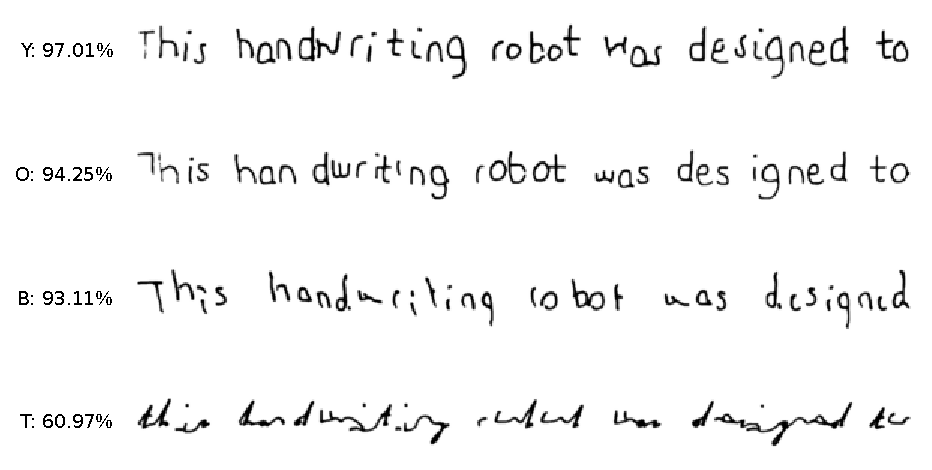
\includegraphics[width=0.98\linewidth]{Figures/results_physical_examples.pdf}
\caption{Stored crops from photographed robot pages for Y, O, B and T. The percentages label each writer's aggregate character score, not the accuracy of the single strip shown. These physical-output examples illustrate the range rather than constituting a new controlled same-sentence experiment.}
\label{fig:res-physical}\end{figure}

The automated reader recovers 84.41\% character accuracy overall, with 45.97\% positional word match. The writer is correctly identified on 159/184 lines (86.41\%), and all fourteen archived page pools are attributed correctly. Seven writers exceed 85\% character accuracy. Y, 150, O and B exceed 93\%, and Y, O, B and 384 exceed both 85\% character accuracy and 85\% line-level writer identification. These are demonstrated operating cases, rather than replacements for the pooled result.

The new physical style comparison applies the same fixed descriptor definitions to the 184 reproduced lines and 156 original validation lines, grouped by the eleven writers. All lines return usable descriptors and no writer is excluded. Original and reproduced text content is not matched sentence by sentence, so the comparison concerns writer-level geometry across these samples. Nine descriptors include pen-dependent ink density and stroke width; the seven shape descriptors omit those two quantities, consistently with the constant-pen design rationale.

Table~\ref{tab:res-physical-style} gives both variants. Standardising each feature across writers separately in the original and physical domains, then correlating the flattened arrays, gives 0.713 over all nine features and 0.697 over seven shape features. With original-domain statistics used for both arrays, the corresponding values are 0.633 and 0.611. Appendix~\ref{app:res-physical-style} gives the extraction and individual descriptors. This is a new retrospective measurement of saved physical output, not an extension of the earlier ten-writer synthetic experiment.
\begin{table}[!htbp]\centering\small
\begin{tabular}{lrrr}\toprule
\textbf{Feature set} & \textbf{Features} & \textbf{Separate domains} & \textbf{Absolute variant}\\\midrule
All geometric descriptors & 9 & 0.713 & 0.633\\
Shape descriptors (ink omitted) & 7 & 0.697 & 0.611\\
\bottomrule\end{tabular}
\caption{New physical-to-original comparison across eleven writers. The first correlation standardises features separately in each domain; the absolute variant uses original-domain statistics for both. The target reference is 0.85.}\label{tab:res-physical-style}
\end{table}


The physical slant coefficient is 0.991, ascender extent 0.817, character width 0.798 and word gap 0.486. For example, writer 150's mean estimated slant changes from $-5.17^\circ$ in the original reference lines to $-5.42^\circ$ in the physical output, approximately $-0.26^\circ$. Across equally weighted, separately standardised features, the pooled shape correlation is the mean of the seven per-feature correlations; their sum 4.8767 divided by seven gives 0.6967. It lies 0.1533 below the 0.85 reference.

\resstep{Observations}
The pooled character score is 0.59 percentage points below the 85\% target. Writer scores vary from 60.97\% to 97.01\%. The character score and writer-identification score do not rank writers identically: T is identified on every scored line while its character score is the lowest, and writer 150 has 96.75\% character accuracy with 53.85\% identification. Thus the two outputs measure different properties of reproduction.

The measured components-per-character descriptor of genuine handwriting is positively associated with reproduced character accuracy ($r=0.855$, Spearman $\rho=0.845$, eleven writers); a lower descriptor indicates more joined handwriting. The corresponding writer-identification rank association is $\rho=-0.027$. These are cross-writer associations, not measurements of the loss caused by an individual joining operation.

\resstep{Statistical analysis}
The descriptive Wilson interval on 159/184 identifications is 80.7--90.6\%. A 10\,000-repeat resampling of the eleven whole writer groups gives a central 95\% range of 77.82--90.27\% for pooled character accuracy. The new physical shape coefficient has a central writer-resampling range of 0.555--0.827. These ranges reflect sensitivity to which observed writers are represented. Shared texts, profiles and capture conditions limit an interpretation as independent generalisation trials. The final targets are assessed using the observed pooled scores and their breakdowns, without claiming a universal pass from the better individual cases.

\reportqt{qt:r2}{Reading handwritten content and identifying its writer (R2)}
\resstep{Objectives of the test or experiment}
Measure the two classification outputs against the 95\% target using data excluded from weight updates for the relevant network. The reader and writer model have different training populations, so their scores are reported separately rather than multiplied into an invented combined accuracy.

\resstep{Equipment used}
The saved IAM line corpus and photographed line crops; the evaluated scratch reader and joint-reader comparison; the 0.17-normalised eleven-writer model; and the transcript-scoring and per-line writer-classification tools on the development host. No gantry movement is required during this scoring stage.

\resstep{Test setup and experimental parameters}
The reader evaluation contains the distributor's 976 IAM validation lines (42\,072 characters) and 100 photographed validation lines (3\,675 characters). The latter use the recorded seeded 15\% line split. Transcript lookup found that many lines from IAM writers 150, 152 and 153 occur in the public training partition; their project-page scores are therefore not used as additional reader validation. The selected photographed and public validation sets are kept distinct. Validation data may have informed checkpoint selection, so these scores describe validation performance rather than a newly collected blind final test.

The writer evaluation contains 156 lines: a held-out labelled page for each of six database writers and the seeded photographed-line split. Photographed validation lines may share a writing session and page background with training lines. This is the split described in Section~\ref{sec:des-class}; its population is stated explicitly when interpreting the result.

\resstep{Steps followed in the test or experiment}
\begin{enumerate}\setlength{\itemsep}{1pt}
\item Check the reader evaluation transcripts against the public corpus partitions and retain the specified validation populations.
\item Read each validation line with greedy CTC decoding and retain the raw edit and reference counts.
\item Classify each writer-validation crop after the selected stroke normalisation; retain its reference, predicted class and confidence.
\item Aggregate by population and writer, and pool each writer's validation lines for the separate group-level result.
\end{enumerate}

\resstep{Results or measurements}
Table~\ref{tab:res-r2-reader} gives the reader scores. The scratch checkpoint yields 94.39\% pooled character accuracy, while the joint reader yields 94.06\% on the same population. The photographed subset yields 94.42\% with the scratch reader and 93.33\% with the joint reader. The author selects the library-trained joint reader for the demonstration. The comparison therefore supports the numerical implementation without substituting its result for the selected system.
\begin{table}[!htbp]\centering\small
\begin{tabular}{lrrrr}\toprule
\textbf{Evaluation set} & \textbf{Lines} & \textbf{Characters} & \textbf{Joint / \%} & \textbf{NumPy / \%}\\\midrule
Public IAM validation & 976 & 42072 & 94.12 & 94.39\\
Photographed A & 31 & 934 & 94.00 & 94.65\\
Photographed B & 19 & 739 & 95.81 & 97.70\\
Photographed O & 22 & 1017 & 94.40 & 94.79\\
Photographed T & 11 & 345 & 85.51 & 89.28\\
Photographed Y & 17 & 640 & 92.03 & 92.50\\
All & 1076 & 45747 & 94.06 & 94.39\\
\bottomrule\end{tabular}
\caption{Character accuracy of the selected library-trained joint reader and the evaluated NumPy-trained reader, using greedy CTC decoding. The public set is the distributor's validation partition, not an independent final test set.}\label{tab:res-r2-reader}
\end{table}


The library-trained writer model correctly classifies 153/156 lines, or 98.08\%. Pooling the available validation lines gives the correct identity for all eleven writers. The individual correct counts are 8/9, 7/8, 9/9, 12/12, 10/10 and 8/8 for the six database writers, and 31/31, 18/19, 22/22, 11/11 and 17/17 for A, B, O, T and Y. Figure~\ref{fig:res-holdout} gives the complete confusion matrix rather than only the overall percentage.
\begin{figure}[!htbp]\centering
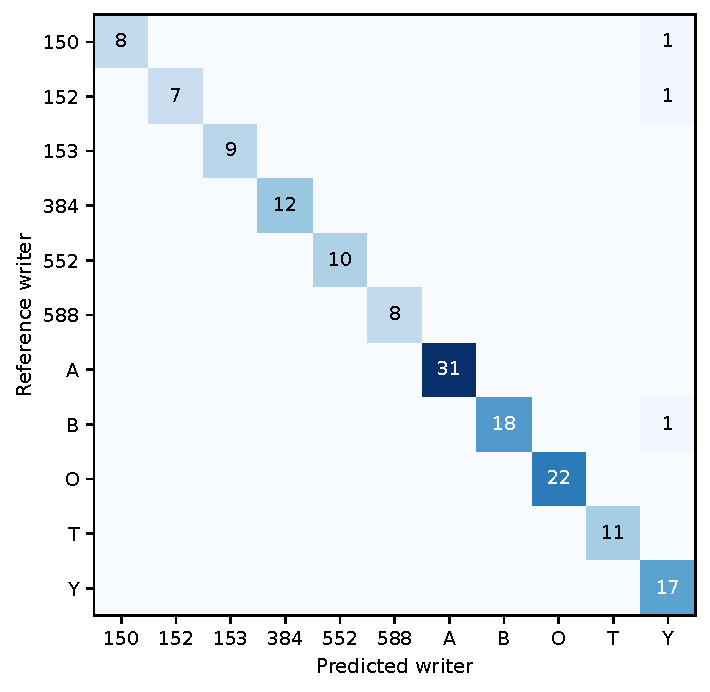
\includegraphics[width=0.84\linewidth]{Figures/results_holdout_confusion.pdf}
\caption{Writer classification on 156 validation lines. Rows are reference writers and columns are predicted writers; blank cells are zero. Three lines are misclassified, all as Y. Photographed writers use the seeded line split, while database writers use held-out pages.}
\label{fig:res-holdout}\end{figure}

\resstep{Observations}
The writer point estimate exceeds 95\% by 3.08 percentage points. The selected reader's pooled text score is 0.94 percentage points below 95\%; the strongest photographed writer's character score under the selected reader is 95.81\%. The selected reader gives 94.12\% on the public subset and 93.33\% on photographed lines, and recovers 221/1\,076 complete lines without an edit. The numerical reader's corresponding character scores are 94.39\% and 94.42\%, with 242 exact lines. The selected and numerical readers have pooled positional word-match scores of 72.16\% and 73.47\%, respectively.

The three writer errors have confidences of 44.2\%, 83.8\% and 39.5\%. Correct lines have mean confidence 97.7\%. The error with 83.8\% confidence shows that a high posterior is not a guarantee of correctness. The error indices are the last entries of their writer's evaluation group; this ordering alone does not establish a physical last-line or short-text cause for the randomly selected photographed subset.

\resstep{Statistical analysis}
The descriptive Wilson interval on writer accuracy is 94.5--99.3\%, and the interval on 11/11 correct writer pools is 74.1--100\%. The observed point estimates are strong, while the lower limits do not establish a population-wide 95\% guarantee. Treating all six predictions below 80\% confidence as wrong, in addition to the one higher-confidence error, leaves 149/156 correct (95.51\%); this is a sensitivity calculation on the same sample, not a measured rejection policy. For character accuracy, Equation~\ref{eq:res-char} is an edit ratio, so a binomial confidence interval on 45\,747 independent characters is not used.

\reportqt{qt:r3}{Complete reproduction time on the embedded platform (R3)}
\resstep{Objectives of the test or experiment}
Compare complete recorded reproduction times with the proposal allowance $4x$~s. The relevant operation includes generation and physical drawing, rather than physical motion alone.

\resstep{Equipment used}
The ODROID N2+, gantry and server stage timer. The primary measurement is the retained server log, including program-end and stop messages. No development-host inference benchmark supplies the physical timing result.

\resstep{Test setup and experimental parameters}
Generation and drawing use separate requests. The drawing request carries generation stages into its recorded reproduction total, as described by the job timing boundary in Section~\ref{sec:des-integration}. The primary analysis selects console records containing a drawing stage, a positive character count and an explicit successful program-end marker. Stopped jobs, zero-character commissioning shapes and unconfirmed summary-only entries are excluded from the pass count. Repeated records refer to recorded requests, not an assumed random sample of all possible text and styles.

\resstep{Steps followed in the test or experiment}
\begin{enumerate}\setlength{\itemsep}{1pt}
\item Associate a reproduction timer block with the preceding physical job's terminal status.
\item Retain explicitly completed positive-character jobs and read the recorded total and character count.
\item Calculate $t/x$ and compare $t$ with $4x$ for each retained record.
\item Group by text length and report the worst recorded total in each group.
\end{enumerate}

\resstep{Results or measurements}
Table~\ref{tab:res-r3-confirmed} and Figure~\ref{fig:res-r3} give 25 completion-confirmed records. Every retained total meets its numerical allowance. The largest normalised time is $166.61/43=3.8747$~s per character, leaving $172-166.61=5.39$~s on that request. At 378 characters the nine confirmed totals range from 507.57~s to 1\,085.01~s, against 1\,512~s allowed.
\begin{table}[!htbp]\centering\small
\begin{tabular}{rrrrr}\toprule
\textbf{Characters} & \textbf{Records} & \textbf{Allowance / s} & \textbf{Worst total / s} & \textbf{Worst / s per char}\\\midrule
43 & 9 & 172 & 166.61 & 3.875\\
75 & 1 & 300 & 188.60 & 2.515\\
82 & 3 & 328 & 260.33 & 3.175\\
91 & 2 & 364 & 222.63 & 2.446\\
132 & 1 & 528 & 277.90 & 2.105\\
378 & 9 & 1512 & 1085.01 & 2.870\\
\bottomrule\end{tabular}
\caption{ODROID reproduction records with explicit program-end confirmation. Generation and drawing are included in the recorded total. All 25 retained records meet their allowances.}\label{tab:res-r3-confirmed}
\end{table}


\resstep{Observations}
The shortest tested length has the narrowest worst-case margin: 3.1\% of its allowance. The longest tested paragraph has a worst-case margin of 28.2\%. The times for the same paragraph vary by a factor of 2.14. The log includes coordinate-clamping messages in some jobs, so completion of the interpreter and satisfaction of the timer do not by themselves prove that every intended trajectory remained unchanged. Character fidelity is assessed separately in QT~1.

\resstep{Statistical analysis}
All 25 confirmed records pass; their descriptive Wilson interval is 86.7--100\%. This is not a claim that future failure has been excluded. The experiment covers six observed lengths from 43 to 378 characters, with one to nine records per length. It provides no direct timing result for shorter requests or a probability of compliance across unseen styles.

\reportqt{qt:r4}{Time to decode a photographed page and identify its writer (R4)}
\resstep{Objectives of the test or experiment}
Compare the embedded classification request with $2+0.025x$~s and identify the time available for a practical improvement. Supporting acceleration experiments retain output checks alongside time measurements.

\resstep{Equipment used}
The ODROID server and stage timer for the two actual requests; the development host for the preserved comparison of sequential NumPy inference with batched PyTorch inference and for the image-resolution experiment. These are different timing platforms.

\resstep{Test setup and experimental parameters}
The ODROID log reports 500 characters over 16 lines and 982 characters over 22 lines. Their recorded totals include loading, conditioning, segmentation, cropping, reading and writer classification. Allowances below use the logged character counts; independent ground-truth counts and any acquisition latency outside the timer are not established by those records. The combined time is the pass criterion. Grouping image and network stages helps diagnose the overrun; it does not impose an additional independent specification on each group.

\resstep{Steps followed in the test or experiment}
\begin{enumerate}\setlength{\itemsep}{1pt}
\item Extract each recorded ODROID classification total and its component stages.
\item Compute the allowance from the recorded count and compare the total with it.
\item For the separate acceleration study, process the same stored pages with the same network weights and compare time and decoded text.
\item Repeat image preparation at half linear resolution, retaining line counts, failed pages and agreement with full-resolution output.
\end{enumerate}

\resstep{Results or measurements}
Table~\ref{tab:res-r4-times} and Figure~\ref{fig:res-r4} show the two ODROID requests. Neither meets R4: $46.26/14.50=3.19$ times the allowance and $55.49/26.55=2.09$ times the allowance. The network stages account for approximately 67.6\% of their combined time, and image stages 32.4\%.
\begin{table}[!htbp]\centering\small
\begin{tabular}{lrr}\toprule
\textbf{Recorded quantity} & \textbf{500 characters} & \textbf{982 characters}\\\midrule
Loading / s & 0.63 & 0.53\\
Conditioning / s & 6.61 & 6.04\\
Segmentation / s & 4.29 & 5.59\\
Cropping / s & 4.61 & 4.65\\
Image stages / s & 16.14 & 16.81\\
Reading / s & 19.02 & 24.66\\
Writer classification / s & 11.09 & 14.01\\
Network stages / s & 30.12 & 38.67\\
Total / s & 46.26 & 55.49\\
R4 allowance / s & 14.50 & 26.55\\
Overrun / s & 31.76 & 28.94\\
\bottomrule\end{tabular}
\caption{Two recorded ODROID classification requests. Totals are taken from the timer; rounded stage values may differ by 0.01 s when summed.}\label{tab:res-r4-times}
\end{table}


On fourteen stored pages, the development-host network experiment records 359.8~s for sequential NumPy inference and 130.3~s for equivalent library modules batched by page, a measured factor of 2.76. Decoded text agrees on every evaluated line. Both the execution backend and the batching strategy change together, so the factor cannot be assigned to batching alone. Writer-label equivalence is not established merely by identical reader text.

The image-resolution experiment finds 247 lines at full resolution and 182 at half resolution across the twelve pages that return results at both scales. None of those twelve retains its line count, and two additional reduced-resolution pages fail to return a segmentation. The reported 4.37-fold image-stage speed factor accompanies a mean text-agreement score of 33.8\%, so it is not an equivalent-output replacement. These comparisons are recorded in Appendix~\ref{app:res-speed}.

\resstep{Observations}
The observed network cost is 60.2 and 39.4~ms per logged character. Applying the host's 2.76-fold factor to those stage times would give 21.8 and 14.3~ms per character, respectively. These are useful design projections, not ODROID measurements. With unchanged image stages, even that projection gives totals of approximately 27.05~s and 30.82~s, still above the two allowances. A faster network path alone therefore does not close the demonstrated total-time gap under this projection.

\resstep{Statistical analysis}
Two ODROID requests establish two observed overruns; they do not establish a timing distribution or failure at every possible page length. The development-host comparison contains fourteen page conditions rather than repeated controlled ODROID runs. Its factor supports an optimisation candidate, while the embedded speed gain and complete R4 pass require direct measurement. A C or C++ implementation is not credited with an unmeasured speed-up.

\reportqt{qt:r5}{Gantry dimensional accuracy and geometric consistency (R5)}
\resstep{Objectives of the test or experiment}
Measure the drawn geometry relevant to the 0.5~mm positional target and distinguish dimensional checks from complete absolute-position and repeatability qualification.

\resstep{Equipment used}
The calibrated gantry, pen and paper; a metal non-digital vernier caliper, whose make, model and least count are not present in the retained record; and the generated 100~mm square and isosceles triangle of 80~mm base and nominal 40~mm height. The physical readings are author-recorded inputs, not outputs that can be regenerated by a script.

\resstep{Test setup and experimental parameters}
The retained measurements are from one square and one triangle after calibration. Four square sides and three triangle sides are compared with their commanded lengths. Caliper least count is not assumed from the number of digits typed in a result; reading uncertainty also depends on finite-width pen marks. The geometry provides a useful commissioning check for the coordinate and stepping model in Section~\ref{sec:des-drive}.

\resstep{Steps followed in the test or experiment}
\begin{enumerate}\setlength{\itemsep}{1pt}
\item Home and calibrate the gantry, then execute the square and triangle jobs.
\item Measure each reported side and calculate its difference from the nominal length.
\item Compare the dimensional differences with 0.5~mm and calculate the mean square-side error.
\item Use the unequal triangle sides to estimate an apparent apex offset under the stated geometric assumptions.
\end{enumerate}

\resstep{Results or measurements}
Table~\ref{tab:res-r5-lengths} retains all seven original readings. Figure~\ref{fig:res-geometry} shows their signed length errors. The four square sides have a mean absolute error of $(0.30+0.20+0.10+0.10)/4=0.175$~mm and maximum 0.30~mm. The largest absolute feature-length difference across both shapes is $|56.20-\sqrt{40^2+40^2}|=0.369$~mm.
\begin{table}[!htbp]\centering\small
\begin{tabular}{llrrr}\toprule
\textbf{Shape} & \textbf{Feature} & \textbf{Nominal / mm} & \textbf{Measured / mm} & \textbf{Error / mm}\\\midrule
Square & Bottom X & 100.00 & 100.30 & +0.30\\
Square & Top X & 100.00 & 100.20 & +0.20\\
Square & Left Y & 100.00 & 100.10 & +0.10\\
Square & Right Y & 100.00 & 99.90 & -0.10\\
Triangle & Base & 80.00 & 80.30 & +0.30\\
Triangle & Left slope & 56.57 & 56.20 & -0.37\\
Triangle & Right slope & 56.57 & 56.90 & +0.33\\
\bottomrule\end{tabular}
\caption{Author-recorded dimensions from one calibrated square and one triangle. These are feature-length errors, rather than an absolute coordinate-error map.}\label{tab:res-r5-lengths}
\end{table}


Place the measured base endpoints at $(-b/2,0)$ and $(b/2,0)$ and the apex at $(d,h)$. Subtracting the two squared-distance equations gives the project's geometric diagnostic:
\begin{equation}
d=\frac{\ell^2-r^2}{2b},\qquad \phi_{\rm app}=\arctan(d/h).
\label{eq:res-apex}
\end{equation}
Using $b=80.30$~mm, $\ell=56.20$~mm, $r=56.90$~mm and the nominal $h=40$~mm gives $d=-0.493$~mm and $\phi_{\rm app}=-0.706^\circ$. The angle is conditional on the assumed height and a shear interpretation; it is not an independent measurement of rail squareness. Both an ideal square and a rhombus can have equal side lengths, which is why diagonal or coordinate measurements would add information absent from the square-side test.

\resstep{Observations}
Every measured feature length is within 0.5~mm of nominal. The two horizontal square sides are long by 0.20--0.30~mm, while the vertical sides straddle nominal by 0.10~mm. The unequal sloping triangle sides are consistent with lateral geometric asymmetry. The measurements do not isolate scale, shear, pen width and reading uncertainty into separate physical causes.

\resstep{Statistical analysis}
There is one specimen of each shape. The spread among sides is not repeated-draw variability, and no standard deviation of repeatability is assigned. Side lengths alone also leave a rigid translation undetected, so the 0.5~mm absolute point-position requirement is not fully proven. The positive result is a dimensional error below the numerical limit on every measured feature; repeated word overlays and bed-coordinate measurements would complete the distinction requested in the proposal.

\reportqt{qt:r6}{Storage and use of multiple trained styles (R6)}
\resstep{Objectives of the test or experiment}
Confirm at least ten represented writers, stored glyph mappings and the ability to use those mappings for reproduction.
\resstep{Equipment used}
The evaluated eleven-class writer checkpoint, stored style profiles and glyph libraries, saved generated jobs and fourteen physical output pages.
\resstep{Test setup and experimental parameters}
The required count is ten. The evaluated set is 150, 152, 153, 384, 552, 588, A, B, O, T and Y. Both class identities and stored trajectory libraries are checked.
\resstep{Steps followed in the test or experiment}
Compare the classifier mapping with the stored profiles, then confirm that every identity occurs in the writer-validation records, physical pages and generated jobs.
\resstep{Results or measurements}
Eleven identities have classifier entries and stored profiles. All have physical samples in Figure~\ref{fig:res-writers} and correct pooled identities in QT~2, exceeding the required count by one.
\resstep{Observations}
The result demonstrates concurrent use of multiple stored styles; QT~1 measures their different reproduction quality.
\resstep{Statistical analysis}
This is an inventory count, so a sampling interval is inapplicable. R6 is met by the evaluated eleven-style set.

\subsubsection{Qualification under the proposal's field conditions}
\label{sec:res-conditions}
Indoor captures and physical drawings demonstrate operation in the fixed test arrangement. The author reports successful operation across lighting conditions wider than the planned range, but no illuminance readings or surface-level/vibration measurements accompany the retained records. The evidence supports the observed bench conditions and capture examples in Section~\ref{sec:des-segverify}; it does not numerically establish the 400--1000~lux endpoints. Table~\ref{tab:res-summary} compares the retained evidence with the proposal's exact environmental conditions.
\FloatBarrier

\clearpage
\renewcommand{\eprthepartname}{Discussion}
\section{Discussion}
\label{sec:discussion}
\subsection{Critical evaluation of the design}
\label{sec:dis-critical}
The project connects photographed handwriting, numerical recognition, persistent writer profiles and a working Cartesian gantry. The results support this central function across eleven writers, with quality depending on the handwriting and embedded classification time remaining the principal performance constraint. This evaluation relates those outcomes to the decisions explained in Design.

\subsubsection{Interpretation of results}
\label{sec:dis-interpretation}
\paragraph{Useful reproduction is demonstrated, with a clear operating range.}
The 84.41\% read-back character score is close to the 85\% target, but its engineering meaning becomes clearer when the eleven writers are separated. Seven exceed 85\% and four exceed 93\%; those four include both personal contributors and a database writer. Thus the method is capable of substantially better than the pooled target on demonstrated styles. The lower scores on other writers show that the remaining improvement concerns consistency across styles, rather than an inability of the gantry to produce readable text at all. Figure~\ref{fig:res-physical} grounds this distinction in physical output.

The association between components per character and legibility is consistent with the limitations of the chosen representation. A glyph library stores observed character shapes and assembles them into new contexts. In more joined handwriting, the appearance of a character can depend strongly on its neighbours, so a cut glyph and a generic connection need not reproduce the same local shape. The observed rank association of 0.845 supports investigating this mechanism, but eleven writers do not isolate joining from glyph coverage, input quality or reader preference. The corresponding identification association is close to zero; it shows that a writer can remain identifiable even where individual characters are difficult for the reader.

The 86.41\% line-identification score and correct attribution of all fourteen page pools are useful evidence that writer-specific structure survives the full physical process. They answer a different question from stylistic correlation. The new physical geometric study gives seven-feature shape correlation 0.697 and nine-feature correlation 0.713, both below 0.85. It also identifies useful retained structure: slant tracks at 0.991, while ascender extent and character width track at approximately 0.817 and 0.798. Word spacing, at 0.486, is a weaker channel. These values motivate improving layout and context while preserving the successful orientation and glyph information; they do not establish that layout is the sole source of loss.

The writer model also participates in candidate selection, so it cannot be treated as an independent aesthetic judge of that selection. The geometric study uses no neural classifier, although it still depends on its descriptor definitions and the different original and reproduced texts. Its separately standardised coefficient primarily describes cross-writer ordering, and the lower 0.611 absolute shape variant shows that agreement of feature magnitudes is more demanding. Automated read-back is likewise an instrument-dependent measure of legibility. It provides a repeatable comparison, while a blinded human reading and style assessment would test the human-facing interpretation of the proposal more directly. Neither the physical overlay nor a human rating is inferred from model confidence.

\paragraph{The classifier results support the chosen architecture.}
The selected joint reader achieves 94.06\% pooled character accuracy, 0.94 percentage points below the 95\% target; the NumPy-trained scratch reader achieves 94.39\% on the same evaluation. The scratch reader's public and photographed subsets score 94.39\% and 94.42\%, while the joint reader scores 94.12\% and 93.33\%. These results show that the line-recognition architecture works on both distributor-cut IAM lines and the project's photographed material. Similar averages do not prove that segmentation is harmless: different text, writers and image conditions may compensate in the mean, and the study does not measure the segmentation contribution separately.

The 98.08\% writer-identification point estimate and correct pooling of all eleven writer groups are particularly strong outcomes for the multi-writer objective. The selected 0.17 stroke width makes this result relevant to a pen plotter that cannot reproduce each contributor's original ink thickness. The three errors also define the limits of the confidence output: one incorrect classification has an 83.8\% posterior, so confidence can guide review but cannot guarantee an identity. The evaluation is closed set, and its photographed split shares acquisition conditions with the training material; a new session with the same writers would be a stronger deployment check.

The selected library reader is retained as the intended demonstration configuration, while the alternative reader result is reported alongside it. This is a configuration decision rather than evidence that the library route necessarily gives the higher text score. On these data the scratch reader is slightly higher; for writer identification the library-trained model is higher. Keeping both comparisons visible gives a more useful assessment of the implementation than a single claim that one training route is uniformly superior.

\paragraph{The physical timing result is a practical success.}
All 25 explicitly completed positive-character ODROID records satisfy 4~s per character, including generation and drawing. The worst request still has 5.39~s of allowance remaining. This demonstrates usable physical throughput across the recorded 43--378-character range, rather than relying on the G-code generator's nominal feed calculation. That distinction is important because pen transitions, path length, GPIO scheduling and generation time all contribute to the request.

The shortest block has the smallest worst-case margin. Generation work is incurred before the drawing begins, while the allowance grows directly with character count. The measured worst short job includes 26.5~s of synthesis and approximately 3.248~s per character of drawing. Treating those two terms as fixed overhead plus a constant drawing rate would put a break-even length near 35 characters, but this is only a local projection. Search effort, repair and geometry change with the text, so the result motivates a direct short-request test rather than a claim that all shorter requests fail. Coordinate clamping in some recorded jobs also prevents the timing pass being used as a substitute for the separate fidelity result.

\paragraph{The classification-time gap is measurable and actionable.}
The two ODROID classification requests exceed their allowances by 31.76~s and 28.94~s. Approximately two thirds of the combined time is spent in the networks, with the remaining third in image processing. This makes network execution the largest observed optimisation opportunity, while also showing that segmentation alone cannot explain the total overrun. A two-request profile identifies the large contributors; it does not establish a constant cost law for arbitrary pages.

The development-host experiment supplies a concrete alternative: equivalent library networks batched by page are 2.76 times faster in the recorded comparison, with the reader text unchanged. It is reasonable to investigate that route on the ODROID. It is not yet reasonable to report the transferred factor as an embedded timing measurement, because the processor, libraries, thread scheduling and memory behaviour affect it. Even the projection with unchanged image processing leaves the two complete requests above their allowances. The required engineering work is therefore a coordinated reduction of network and image-stage cost, while retaining the output checks.

\paragraph{Mechanical accuracy is promising, with a precise distinction in what was measured.}
Every measured square and triangle feature is within 0.5~mm of nominal, and the square's mean absolute side error is 0.175~mm. These are useful results for the calibrated belt-and-rail mechanism. The triangle's unequal sloped sides additionally suggest an alignment effect that a side-length-only square check cannot expose. The apparent $0.706^\circ$ shear diagnostic offers a direction for adjustment, conditional on the assumed height and other geometric errors.

Neither equal side lengths nor small side-length errors fix the figure's absolute placement on the page. A translated figure can retain the same lengths, and repeated drawings can vary even when one specimen is accurate. The dimensional result should therefore be credited for what it demonstrates: a physically realised coordinate-to-motion path with sub-0.5~mm length differences on the measured features. A repeated-word overlay and a referenced bed-coordinate grid would extend that evidence to the proposal's positional and repetition objectives.

\paragraph{Relationship to published approaches.}
The sequence reader follows the CNN--BiLSTM--CTC architecture discussed by K{\i}z{\i}l{\i}rmak and Yan{\i}ko{\u g}lu~\cite[pp.~4--5]{kizilirmak2023}. The project's measured CER is 5.94\% for the selected reader and 5.61\% for the scratch reader, obtained directly from Equation~\ref{eq:res-char}. This is evidence of a functioning implementation in the same task family. It is not a controlled ranking against a published test result: the distributor's validation partition, training mixture, checkpoint selection and decoding protocol are not a matched published test protocol. In particular, the positional word-match score here is not directly comparable with published WER.

The reproduction strategy has a closer practical relationship to example-based approaches. Haines et al. demonstrate synthesis using a small collection of handwritten pages and explicit extracted forms~\cite[p.~4]{haines2016}. That supports the use of a small personal dataset as a design rationale without establishing an identical output quality. Graves's sequence generator uses ordered pen-coordinate observations~\cite[p.~18]{graves2013}; this project starts with offline photographs and does not observe those temporal paths. Modern image generators can model richer context, including One-DM's use of a single reference at generation time, but that reference count must be distinguished from the corpus and hardware used to train the generator~\cite[p.~9]{dai2024}. These comparisons explain the selected scope: an inspectable geometric system built from the available data, with context modelling as its principal reproduction trade-off.

\subsubsection{Critical evaluation}
\label{sec:dis-choices}
\paragraph{Separating the implementation contribution from checkpoint selection.}
The project implements convolution, normalisation, recurrent operations, CTC and optimiser updates numerically, as documented in Section~\ref{sec:des-implementations}. It also has a framework route for training the corresponding architecture. Choosing the library-trained writer for the demonstration does not remove the first-principles work; the numerical checks and trained-model comparison provide separate evidence for it. Conversely, the existence of a numerical trainer does not establish that every selected checkpoint came from that trainer.

Table~\ref{tab:dis-training} compares the saved models on common material. The numerical writer model exceeds the 95\% target as an observed line-level result, reaching 149/156 or 95.51\%, while the library-trained model reaches 153/156 or 98.08\%. On the 185-crop physical-output comparison the difference is larger, 80.54\% against 85.95\%. Both numerical and library checkpoints therefore learn useful writer distinctions, with the selected model providing the stronger measured writer result on these two populations. The 185-crop comparison is kept distinct from the 184 paired lines of QT~1.

\begin{table}[!htbp]\centering\small
\begin{tabular}{lrr}\toprule
\textbf{Common evaluation} & \textbf{Library trained} & \textbf{NumPy trained}\\\midrule
Writer: original validation lines & 153/156 (98.08\%) & 149/156 (95.51\%)\\
Writer: physical-output crops & 159/185 (85.95\%) & 149/185 (80.54\%)\\
Writer: original groups correct & 11/11 & 11/11\\
Writer: physical writer groups correct & 11/11 & 10/11\\
Reader: pooled character accuracy & 94.06\% & 94.39\%\\\bottomrule
\end{tabular}
\caption{Saved trained-model comparison. The reader row compares the joint and evaluated scratch checkpoints. The writer rows use matched crops and the same 0.17 preprocessing; these are comparisons of particular trained models, not an isolation of training precision or framework effects.}
\label{tab:dis-training}\end{table}

The supplied numerical-writer training log records 1\,031 training and 155 validation lines, a best displayed validation accuracy of 0.968 by epoch 41, and approximately 19--23~minutes per reported epoch. The reader excerpt records approximately 111--122~minutes per reported epoch and a resume from an existing numerical checkpoint. The later writer re-evaluation has 156 lines because the extraction and transcript correspondence used in that evaluation differs from the training-era population. Its 95.51\% result should therefore not be substituted for the 96.8\% training-validation figure or vice versa.

The reported float32 training choice is consistent with the need to limit the cost of these numerical runs, but this experiment does not isolate precision as the cause of an accuracy difference. Higher arithmetic precision does not, by itself, establish a higher trained-model classification score. A controlled precision study would require the same initial weights, sample order, preprocessing, optimiser settings and stopping rule. The existing fixed-parameter numerical checks support the implementation's arithmetic separately from these trained-model comparisons.

\paragraph{Line recognition addresses a real weakness in character isolation.}
The proposal described separating characters or connected groups before classification. The implemented reader instead recognises lines, while known-transcript CTC alignment recovers character boundaries during profile construction. This was a defensible response to connected handwriting: uncertain character cuts are not made a prerequisite for reading the text, and CTC supports training from complete transcripts~\cite[pp.~2--3]{graves2006}. The cost is a larger sequence model and continued dependence on correct line ownership. The Results therefore qualify the final line-based design while retaining the functional contribution promised in the proposal.

\paragraph{The glyph library fits the data and exposes its own limitations.}
An explicit library permits size, slant, spacing and machine coordinates to be examined directly. It also allows the same stored writer to be used for different text without fitting a new generator for each request. These advantages are borne out by eleven functioning profiles and the different physical outputs. The price is a finite set of observed shapes, with limited information about how a writer changes a letter between neighbours. Multiple-character units or context-conditioned variants would address that loss more directly than increasing candidate count alone. They would also need reliable extraction and enough examples of the relevant combinations.

The first-principles and embedded-processing commitments of the proposal also constrain the interpretation of a library speed remedy. A framework benchmark is a useful engineering comparison; it does not by itself establish compliance with the original library restriction. A batched numerical implementation could retain that contribution, while compiled kernels for the identified hot loops offer a second route. Neither has an embedded compliance result in the present measurements. The practical workflow also separates off-device training from embedded operation. The supplied training records substantiate the numerical implementation and the cost of model preparation, while the proposal's intended embedded training mode is not demonstrated by those off-device runs. This distinction keeps the substantial implementation contribution and the final operating arrangement clear.

\paragraph{Economic feasibility.}
The author's current build-cost estimate is approximately R4\,000. The ODROID was borrowed at no purchase cost and will be returned after the project. This reduces the prototype's cash expenditure, but a replacement board would be part of a reproducible deployment cost. The ledger and subsequent purchases require reconciliation before a precise total is claimed; the later listed clipboard, paper, pen and estimated training electricity amount to R750 and may overlap the approximate estimate. The electricity amount is an author estimate, not an energy-meter result.

Using the available board allowed the project to prioritise the complete mechanical and image-processing system. The cost choice is relevant to the available compute, although the measurements do not show what a different board would have achieved. The 2.76-fold development-host comparison is stronger evidence for a software optimisation opportunity than an unsupported assertion that a more expensive platform would necessarily meet R4. A future cost comparison should include hardware, development effort and the measured quality retained by each acceleration route.

\subsubsection{Unsolved problems}
\label{sec:dis-unsolved}
The main reproduction problem is the variation between writers. Improvements should target the poorer cases without losing the high-performing printed and lightly joined styles. A useful next experiment would keep the reader, writer model and input text fixed while comparing current single-glyph paths with selected multi-character units. That would test the proposed context explanation directly. The new geometric study establishes a physical-output baseline; matching original and reproduced sentences and repeating capture sessions would better separate writer fidelity from content and acquisition effects.

The timing problem requires equivalent-output optimisation. The reduced-resolution experiment is valuable precisely because it measures the cost: it returns fewer lines on every comparable page and fails to segment two pages. It therefore cannot be accepted simply because its projected total may fall below an allowance. The better sequence is to preserve the reference output, measure the ODROID's hot loops and memory use, then compare a batched numerical route or selected compiled routines against that reference. The stopping criterion should be the complete request allowance together with unchanged transcripts and an agreed writer-output check.

The remaining mechanical work is a stronger positional qualification rather than an unsupported redesign. Frame squaring, belt consistency and pen-holder stiffness are plausible sources of geometric error, but the present length measurements do not rank them conclusively. Measuring repeated grid points, both square diagonals and the proposal's repeated word would identify where calibration is sufficient and where a mechanical adjustment is needed. A more controlled pulse scheduler and acceleration profile are sensible extensions of the motion design, but their benefit must be assessed on completed drawings rather than inferred from commanded feed.

The model files, preprocessing width and stored writer mappings must also be carried into the demonstration as one identified configuration, so that a changed checkpoint does not silently change the meaning of the report's results.

\subsubsection{Strong points of the design}
\label{sec:dis-strengths}
The functioning chain is a principal strength: the system captures pages, recognises text, identifies writers, stores trajectories and produces real handwriting. Eleven styles are exercised in recognition and physical reproduction, seven exceed the reproduction character target, and all eleven writer-validation groups are identified correctly when pooled. These results substantiate the multi-writer objective.

An output can be followed through its source crop, normalised glyph, placement and emitted command. The independent G-code checks and physical measurements support this inspectable separation, allowing an improvement to be tested at a known interface while retaining the successful stages.

Operation-level checks and trained results support the numerical implementation: the numerical writer reaches 95.51\% on the common evaluation, and the numerical reader is competitive with the joint reader. The framework route supplies a practical reference and the stronger selected writer model. Together they support the implementation contribution and the final model choice.

\subsubsection{Expected failure conditions}
\label{sec:dis-failures}
Strong cursive connections, scarce character variants and text outside the available alphabet are the most relevant reproduction limits. A profile can preserve only the geometry it contains or the approximations selected for missing characters. Excessive layout extent can also cause clipping or coordinate clamping. A request should therefore be inspected in the preview and validated against the writing area before physical execution; a completed interpreter run alone is not proof of an unchanged trajectory.

For reading, unusually sparse pages, touching lines, page curvature and strong perspective changes can defeat the geometric preparation even when a cropped-line network is accurate. The Design's real capture examples illustrate these conditions. The writer classifier always chooses among its eleven represented identities, so an unfamiliar writer can receive a confident known-writer label. Short or ambiguous lines provide less evidence, while the present confidence sample does not establish a universally safe rejection threshold. Page pooling improves the observed group result but cannot recover information absent from every crop.

The gantry uses open-loop step counts. A missed step changes the physical position without an encoder measurement of that displacement. Limit switches and software abort handling provide useful boundary and stop functions, but depend on the installed switches, electrical circuit and running controller. The installed pen-motor circuit's lack of a flyback diode is a hardware limitation already identified in Section~\ref{sec:des-pen}; repeated reliable operation should not be treated as proof that the switching transient is harmless.

Finally, classification requests outside the tested sizes and very short writing requests have no demonstrated timing envelope. The measured results describe the recorded workload and platform, not all possible text, page sizes or concurrent users. This defines a practical laboratory prototype whose demonstrated successes can be repeated with an identified configuration, and whose extensions have specific measurements to target.

\subsection{Considerations in the design}
\label{sec:dis-considerations}
\subsubsection{Ergonomics}
The browser interface places text entry, captured-page review, writer selection and output preview on the operator's normal screen. Calibration and a writing-area indication reduce setup ambiguity, while the preview permits inspection before movement. Network operation is the selected arrangement; the ODROID also has a display interface~\cite{odroidn2ds}.

The page and pen still require manual positioning, and the motion area must remain accessible for loading while being kept clear during execution. A more complete user flow would confirm the paper restraint, valid calibration, selected profile and preview bounds before a job, and clearly distinguish generation, running, stopped and completed states. These are consequences of combining a software interface with a moving mechanism, rather than cosmetic interface additions.

\subsubsection{Health and safety}
The moving carriage, pulleys and belts present pinch points, and a protruding pen or tool can contact a hand in the working area. The installed end stops, limits, abort handling and controlled setup procedure reduce exposure during normal laboratory operation. The software stop is useful operational control; independent removal of motor power would provide protection if the controller or network became unresponsive. The driver and transistor temperature, wiring restraint and supply enclosure also require attention because the motor circuits carry the actual load currents.

The 24~V motor rail and 3.3~V logic are separate from the mains inputs of the purchased supplies. Low internal voltage does not establish mains insulation or enclosure quality. The supply labels and installed circuit should therefore be part of the final hardware record. A flyback path for the pen motor is a specific improvement supported by the switching analysis already given in Design~\cite{rohmlowside2026}; it is not described as a fitted protection component.

\subsubsection{Environmental impact}
The borrowed ODROID will be returned after the project. Reusable motors, rails, drivers and replaceable printed parts allow components to be repaired or used in other work. The printed-part material is not identified in the retained record, so no material-specific recycling claim is made.

Paper, pens and training electricity are the main recurring consumables identified by the author. Previewing jobs and testing geometry digitally can reduce wasted paper, while real physical tests remain necessary to establish performance. The reported R500 training-electricity allowance is a cost estimate; no total energy or environmental saving is calculated from it without power and runtime measurements. Electronics, plastics and remaining consumables should be separated and handled through appropriate local collection routes at end of life.

\subsubsection{Social and legal impact}
The intended benefit is personalised writing from digital text, including possible use by someone who cannot comfortably produce their own handwriting. The present system demonstrates the technical mechanism; accessibility or clinical benefit has not been evaluated with users. Reproducing another person's style also creates a risk of impersonation. Samples and profiles should be used with permission, and generated material should be identified as machine-produced where its origin matters.

The author confirms that all five personal contributors signed consent forms. Those signatures should be retained securely as supporting records; publishing them in the report would unnecessarily expose identifying material. Identifiable handwriting and writer profiles require consideration under South Africa's Protection of Personal Information Act, including minimal collection, a lawful processing basis, retention limits and security safeguards~\cite[pp.~8--9, 11]{popia2013}. Consent is one lawful basis and does not itself establish every aspect of compliance. The applicable database terms must also accompany use of the IAM material. The local-network server and stored profiles should have access restricted to the intended operator; the prototype is not presented as a publicly secured handwriting service.

\subsubsection{Ethics clearance}
Signed consent was obtained from the five personal contributors. No institutional clearance or exemption reference is included in the retained records; participant consent is not presented as evidence of institutional approval.
\FloatBarrier

\clearpage
\renewcommand{\eprthepartname}{Conclusion}
\section{Conclusion}
\subsection{Summary of the work completed}




\subsection{Summary of observations and findings}
    
    

\subsection{Contribution}
    
    

\subsection{Suggestions for future work}
    
    



\clearpage
\renewcommand{\eprthepartname}{References}
\bibliographystyle{IEEEtran}
\bibliography{references}
\clearpage\appendix
\renewcommand{\eprthepartname}{Supporting evidence}

\section{Supporting implementation calculations}
\label{app:des-implementation}
The main Design section explains the engineering decisions and representative operations. This appendix records the derivative conventions, image operations and parameter meanings needed to inspect the numerical implementation in more detail. Algorithms in the main text are explanatory pseudocode; the separately submitted source remains the executable implementation.

\subsection{Numerical network derivatives}
\label{app:des-derivatives}
Applying the backpropagation chain rule~\cite[pp.~3--4]{lecun1998} to a linear layer $Y=XW^T+b$ with incoming derivative $G$, the implemented derivatives are $\partial\mathcal L/\partial X=GW$, $\partial\mathcal L/\partial W=G^TX$ and the sum of $G$ over samples for the bias. Convolution applies the corresponding matrix calculation to overlapping image patches as described in Equation~\ref{eq:des-convback}. Contributions to the same input pixel are summed.

For each batch-normalisation channel, $N=BHW$ values contribute to the batch statistics. The training forward pass uses population variance, while the running variance update uses its $N/(N-1)$ corrected estimate. The running update momentum is 0.1. With $\widehat x=(x-\mu)/\sqrt{\sigma^2+\epsilon}$ and $g=\partial\mathcal L/\partial y$, Equation~\ref{eq:app-bnback} gives the input derivative, obtained by simplifying the batch-normalisation chain-rule expressions~\cite[p.~4]{ioffe2015}.
\begin{equation}
\frac{\partial\mathcal L}{\partial x_i}=
\frac{\gamma}{N\sqrt{\sigma^2+\epsilon}}
\left[Ng_i-\sum_jg_j-\widehat x_i\sum_jg_j\widehat x_j\right].
\label{eq:app-bnback}
\end{equation}

The parameter derivatives accompanying Equation~\ref{eq:app-bnback} are $\sum_i g_i\widehat x_i$ for $\gamma$ and $\sum_i g_i$ for $\beta$. Inference uses stored statistics and requires no batch-dependent update.

ReLU passes an incoming derivative only where its cached input was positive. Spatial max pooling scatters it to the selected maximum in each window. Height-max pooling does the same along height; width averaging distributes the derivative equally over the pooled columns. The implementation uses inverted dropout: it multiplies by the cached Bernoulli mask divided by $1-p$ during training and is the identity at inference. This moves the expected-output scaling from test time to training time relative to the original presentation~\cite[pp.~1931, 1934]{srivastava2014}. Reusing the same mask in the backward calculation is essential.

The LSTM backward pass differentiates the implemented recurrence in Equation~\ref{eq:des-lstm}; full backpropagation through time for this cell form is described by Graves~\cite[pp.~4--5]{graves2013}. It carries both the hidden derivative from the next step and a separate cell derivative. Writing the combined hidden derivative as $d h_t$, Equation~\ref{eq:app-lstmback} shows the dependencies before gate-activation derivatives are applied.
\begin{equation}
\begin{aligned}
d c_t&=d c_t^{\mathrm{next}}+d h_t\odot o_t\odot[1-\tanh^2(c_t)],\\
d o_t&=d h_t\odot\tanh(c_t),& d f_t&=d c_t\odot c_{t-1},\\
d i_t&=d c_t\odot g_t,&d g_t&=d c_t\odot i_t,\\
d c_{t-1}&=d c_t\odot f_t.
\end{aligned}
\label{eq:app-lstmback}
\end{equation}

Sigmoid gates multiply these derivatives by $a(1-a)$; the candidate multiplies by $1-g_t^2$. The concatenated gate derivatives accumulate outer products with $x_t$ and $h_{t-1}$ into the two weight matrices. Multiplication by $W_h$ provides the next reverse-time hidden derivative in Equation~\ref{eq:app-lstmback}. Each bidirectional layer reverses the appropriate sequence and sums the two input derivatives; stacked layers are differentiated in reverse layer order.

The numerical CTC forward score uses the recurrence in Equation~\ref{eq:app-ctcforward}, written in log space from the CTC path recursion~\cite[p.~4]{graves2006}.
\begin{equation}
\alpha_{t,s}=\log p_t(\ell'_s)+
\operatorname{LSE}_{r\in\mathcal P(s)}\alpha_{t-1,r}.
\label{eq:app-ctcforward}
\end{equation}
For frame 11 and the \texttt{V} state in the real Owen line, the predecessor log-forward scores are $-12.8882643$, $-8.9807719$ and $-0.1088294$, and the log emission is $-0.01988985$. Equation~\ref{eq:app-ctcforward} gives $\alpha=-0.01988985+\log(e^{-12.8882643}+e^{-8.9807719}+e^{-0.1088294})\simeq-0.12857619$. This sums the admissible predecessor mass, whereas the main-text forced alignment selects one predecessor.

The predecessor set in Equation~\ref{eq:app-ctcforward} contains the current state, the preceding state and an admissible two-state skip. A skip is excluded when its destination is blank or repeats the label two states earlier. With log scores $a,b$, the stable pairwise reduction is $m+\log(\exp(a-m)+\exp(b-m))$, where $m=\max(a,b)$; the all-unreachable case remains $-\infty$. The backward recurrence uses successor emissions at $t+1$, yielding the occupancy convention in Equation~\ref{eq:des-ctcgrad}.

\subsection{Optimisers and gradient scaling}
The reader uses an uncentred RMSprop accumulator, following the moving-square-gradient principle~\cite[p.~29]{tieleman2012}. The code selects its own averaging coefficient and adds the stated decay term. For parameter $\theta$, raw gradient $g$, learning rate $\eta$ and weight-decay coefficient $\lambda_w$, the implemented update is Equation~\ref{eq:app-rmsprop}.
\begin{equation}
g' =g+\lambda_w\theta,\quad
v_t=0.99v_{t-1}+0.01(g')^2,\quad
\theta_t=\theta_{t-1}-\eta\frac{g'}{\sqrt{v_t}+10^{-8}}.
\label{eq:app-rmsprop}
\end{equation}

Decay in Equation~\ref{eq:app-rmsprop} enters the gradient before accumulation. The writer's AdamW instead uses separate parameter decay, as shown in Equation~\ref{eq:app-adamw}~\cite[p.~2]{kingma2015},~\cite[p.~3]{loshchilov2019}.
\begin{equation}
\begin{aligned}
m_t&=0.9m_{t-1}+0.1g,& v_t&=0.999v_{t-1}+0.001g^2,\\
\widehat m_t&=m_t/(1-0.9^t),&\widehat v_t&=v_t/(1-0.999^t),\\
\theta_t&=\theta_{t-1}-\eta\left(\frac{\widehat m_t}{\sqrt{\widehat v_t}+10^{-8}}+\lambda_w\theta_{t-1}\right).
\end{aligned}
\label{eq:app-adamw}
\end{equation}

Following global gradient-norm clipping~\cite{pascanu2013}, before the writer update all gradient tensors are scaled together by $\min(1,5/\|g\|_2)$, with a numerical denominator guard. Clipping individual tensor norms independently would be a different operation. The numerical reader loop does not apply that clipping. Equations~\ref{eq:app-rmsprop} and~\ref{eq:app-adamw} describe code operations, not a claim that their default learning rates were used in every completed run.

\subsection{Morphology, thinning and path simplification}
For binary mask $M$ and neighbourhood $K$, dilation is the maximum of translated mask values and erosion is their minimum. Closing applies dilation followed by erosion with the same footprint~\cite[pp.~533, 541]{haralick1987}. For a binary mask and symmetric flat footprint, the set operations correspond to neighbourhood maximum and minimum. The implementation obtains rectangular neighbourhood counts through prefix sums; binary comparisons then implement these operations. Connectivity analysis uses horizontal runs and union operations with diagonal overlap admitted, rather than a library component-labelling call.

The thinning conditions follow Zhang and Suen~\cite[p.~237]{zhang1984}. The method inspects the eight neighbours $P_2,\ldots,P_9$ clockwise from north. A removable foreground pixel has two to six foreground neighbours and exactly one background-to-foreground transition around that ring. The two alternating subpasses additionally require, respectively,
\begin{equation}
\begin{array}{ll}
P_2P_4P_6=0,\ P_4P_6P_8=0 &\text{(first subpass)},\\
P_2P_4P_8=0,\ P_2P_6P_8=0 &\text{(second subpass)}.
\end{array}
\label{eq:app-thinning}
\end{equation}
During thinning of the actual Owen crop, the first recorded deletion in subpass one was pixel $(y,x)=(12,190)$ with neighbours $(P_2,\ldots,P_9)=(0,0,1,1,1,1,0,0)$. Its neighbour count is four and its circular transition count is one. Both first-subpass products are zero because $P_2=0$ and $P_8=0$, so the pixel is deleted when the subpass mask is applied. The deletion is applied with the other eligible pixels in that subpass.

Candidates in Equation~\ref{eq:app-thinning} are deleted together in each subpass, and the pair of subpasses repeats until unchanged. This reduces thickness while limiting topology changes; it cannot restore ink already lost during thresholding. The same thinning primitive supports stroke normalisation, glyph tracing and the diagnostic retracing route.

The default tracer begins at graph nodes whose degree differs from two, follows unused pixel edges, and then recovers remaining closed loops. Short dangling spurs are pruned, and nearby chain ends are greedily rejoined when their continuation angle is below $75^\circ$. This remains a geometric estimate rather than a verified natural handwriting order. Polyline simplification compares interior points with the line through the endpoints, retaining a point and splitting recursively when the deviation exceeds tolerance. The code adapts the polyline reduction method~\cite{douglas1973}. Near-closed paths are first split at a distant point so that a zero-length endpoint chord does not collapse the loop. The extraction tolerance is 0.6 source pixels before normalisation; final path smoothing and machine decimation occur in their own coordinate units.

\subsection{Profile and trajectory quantities}
Table~\ref{tab:app-fields} records the fields most likely to be confused during inspection. Full arrays and every tuning constant remain in the source rather than expanding the main text into a variable dictionary.

\begin{table}[!htbp]\centering\small
\begin{tabularx}{\linewidth}{|p{0.27\linewidth}|X|}
\hline\textbf{Quantity}&\textbf{Meaning and unit}\\\hline
\texttt{xHeightPx}&Reference source x-height in pixels; not a physical pen height\\\hline
\texttt{strokes}&Ordered point lists in glyph x-height units; $y$ increases upwards\\\hline
\texttt{width}, \texttt{lead}, \texttt{advance}&Ink width, lead-in and cell/placement extent; distinct x-height quantities\\\hline
\texttt{top}, \texttt{bot}&Vertical extrema relative to the baseline, in x-heights\\\hline
\texttt{connL}, \texttt{connR}&Observed boundary crossings during source extraction\\\hline
\texttt{priorD}&Descriptor distance from the pooled character reference; not writer confidence\\\hline
\texttt{idealMedoid}, \texttt{idealGlyphs}&Actual representative variant and compatible median-stroke prototype\\\hline
\texttt{letterAdvance}&Per-character median source advance; sampled variants retain their own placement geometry\\\hline
\texttt{lineStepMm}&Synthesised baseline spacing before optional machine respacing\\\hline
\texttt{jointScore}&Internal harmonic selection score; not independent stylistic correlation\\\hline
\texttt{clipped}&Count of points clamped by the motion-file conversion; not an acceptable layout target\\\hline
\end{tabularx}
\caption{Selected implementation fields and their interpretation.}
\label{tab:app-fields}
\end{table}

Raw alignment confidence is a path score used for relative filtering, not a calibrated probability of a correct cut. The cross-writer prior uses a median occupancy descriptor, then unit normalisation; its minimum pooled sample count is twelve. Writer consensus retains approximately 75\% of a sufficiently populated pool, with at least three variants. Compatible prototypes group equal stroke counts, resample strokes to 44 points, align them and take robust pointwise summaries. Admission to the variant pool requires prior distance below 0.32 and improvement of more than 0.02 over the median raw distance. These gates reduce malformed geometry but do not prove that a distinctive form is incorrect.

Machine conversion maintains image, glyph, trajectory and machine coordinate frames separately. The line-centre shifts in Equation~\ref{eq:des-machinecoords} are zero when no respacing is requested. Workspace fitting and clipping are distinct: fitting scales the whole trajectory uniformly, while clipping changes individual points and can deform letters. Final file parsing provides a useful conversion check because it reconstructs movements from emitted commands instead of directly displaying the input trajectory again.
\FloatBarrier

\subsection{Detailed training procedures}\label{app:des-training-procedures}
The main chapter retains the model, loss, design choices and representative checks. The following pseudocode records the detailed recurrences and update sequence. Algorithm~\ref{alg:des-ctc} adapts the CTC forward--backward method~\cite[pp.~4--6]{graves2006}; Algorithm~\ref{alg:des-train} assembles the project's training operations.

\begin{designalgorithm}
\caption{Numerical CTC loss and logit gradient}
\label{alg:des-ctc}
\prequire{Logits $z\in\mathbb R^{T\times B\times C}$ and encoded targets.}
\begin{designpseudo}
\pstate{0}{$\log p\leftarrow\operatorname{LogSoftmax}(z)$; $L\leftarrow0$; $g\leftarrow0$}
\pstate{0}{\textbf{for each} batch item $b$ \textbf{do}}
\pstate{1}{$\ell'\leftarrow$ target interleaved with blanks}
\pstate{1}{Initialise $\alpha,\beta$ to $-\infty$; admit first blank and first label}
\pstate{1}{\textbf{for} $t\leftarrow1$ \textbf{to} $T-1$ \textbf{do}}
\pstate{2}{\textbf{for each} state $s$ \textbf{do}}
\pstate{3}{$\alpha_{t,s}\leftarrow\log p_t(\ell'_s)+\operatorname{LSE}_{r\in\mathcal P(s)}\alpha_{t-1,r}$}
\pstate{2}{\textbf{end for}}
\pstate{1}{\textbf{end for}}
\pstate{1}{$\log Z\leftarrow\operatorname{LSE}$ of the admissible final states}
\pstate{1}{Initialise final $\beta$ to zero; recurse backward with next-frame emissions}
\pstate{1}{$q_{t,k}\leftarrow\sum_{s:\ell'_s=k}\exp(\alpha_{t,s}+\beta_{t,s}-\log Z)$}
\pstate{1}{$L\leftarrow L-\log Z$; $g_{t,b,k}\leftarrow(p_t(k)-q_{t,k})/B$}
\pstate{0}{\textbf{end for}}
\pstate{0}{\textbf{return} $L/B,g$}
\end{designpseudo}
\end{designalgorithm}

\begin{designalgorithm}
\caption{One numerical training batch and validation checkpoint decision}
\label{alg:des-train}
\prequire{Training batch, task, parameters $\theta$ and optimiser state.}
\begin{designpseudo}
\pstate{0}{$(X,y)\leftarrow$ task-specific preparation and training augmentation}
\pstate{0}{$(F,\mathcal K)\leftarrow\operatorname{BackboneForward}(X,\theta)$; retain caches}
\pstate{0}{\textbf{if} task is reader \textbf{then}}
\pstate{1}{$(z,\mathcal K_h)\leftarrow\operatorname{BiLSTMHead}(F)$; $(L,g)\leftarrow\operatorname{CTC}(z,y)$}
\pstate{0}{\textbf{else}}
\pstate{1}{$(z,\mathcal K_h)\leftarrow\operatorname{WriterHead}(\operatorname{MeanWidth}(F))$}
\pstate{1}{$(L,g)\leftarrow\operatorname{CrossEntropy}(z,y)$}
\pstate{0}{\textbf{end if}}
\pstate{0}{$g_F\leftarrow\operatorname{HeadBackward}(g,\mathcal K_h)$}
\pstate{0}{$\nabla\theta\leftarrow\operatorname{BackboneBackward}(g_F,\mathcal K)$}
\pstate{0}{\textbf{if} task is writer \textbf{then} clip total gradient norm to $5$}
\pstate{0}{$(\theta,\text{state})\leftarrow\operatorname{OptimiserStep}(\theta,\nabla\theta,\text{state})$}
\pstate{0}{\textbf{if} epoch is complete \textbf{then}}
\pstate{1}{Validate with fixed preparation, stored normalisation and dropout disabled}
\pstate{1}{Update schedule; save progress; replace best only if its criterion improves}
\pstate{0}{\textbf{end if}}
\pstate{0}{\textbf{return} $L,\theta,\text{state}$}
\end{designpseudo}
\end{designalgorithm}

\subsection{Expanded numerical calculation checks}\label{app:des-expanded-checks}

For one image, let $X_c$ contain flattened input patches, so the matrix formulation of convolution gives $Y=WX_c+b$~\cite{chellapilla2006}. Applying the chain rule to $Y_{oj}=\sum_k W_{ok}(X_c)_{kj}+b_o$ gives $\partial\mathcal L/\partial W_{ok}=\sum_j G_{oj}(X_c)_{kj}$ and $\partial\mathcal L/\partial(X_c)_{kj}=\sum_o W_{ok}G_{oj}$. Equation~\ref{eq:des-convback} collects these derived sums in matrix form.
\begin{equation}
\frac{\partial\mathcal L}{\partial W}=GX_c^T,\qquad
\frac{\partial\mathcal L}{\partial X_c}=W^TG.
\label{eq:des-convback}
\end{equation}

Weight and bias derivatives are summed over the batch and output positions. Overlapping patch derivatives in Equation~\ref{eq:des-convback} are added back into the padded input, not overwritten. Max-pool derivatives return to the recorded maxima, width-average derivatives are distributed uniformly, and the LSTM backward pass accumulates both hidden-state and cell-state contributions through time. Appendix~\ref{app:des-implementation} records the remaining derivative conventions and optimiser calculations without repeating the architecture here.

For the traced Owen crop, the first convolution uses one $64\times640$ input and a $3\times3$ kernel. Its patch matrix contains $(1)(1)(3)(3)(64)(640)=368640$ values, requiring $368640\times4/2^{20}=1.40625$\,MiB in float32. This determines one intermediate array's storage, not peak process memory. Later-layer arrays and any training gradients add storage; training and forward-only inference footprints must be assessed separately.

Numerical perturbation provides a finite-difference sensitivity check~\cite[pp.~18--19]{jcgm2008}. For the loss function here, the central-difference expression is derived by subtracting the two Taylor expansions $\mathcal L(\theta\pm\varepsilon e_i)=\mathcal L(\theta)\pm\varepsilon\partial_i\mathcal L+\tfrac12\varepsilon^2\partial_{ii}\mathcal L+O(\varepsilon^3)$. Division by $2\varepsilon$ cancels the constant and even terms, giving Equation~\ref{eq:des-gradcheck} with truncation error $O(\varepsilon^2)$ where the loss is sufficiently smooth. One logit or parameter is perturbed at a time.
\begin{equation}
g_i^{\mathrm{num}}=\frac{\mathcal L(\theta+\varepsilon e_i)
-\mathcal L(\theta-\varepsilon e_i)}{2\varepsilon}.
\label{eq:des-gradcheck}
\end{equation}
For the real Owen line's \texttt{V} logit at frame 11, the two losses with $\varepsilon=10^{-4}$ are $\mathcal L_+=0.4703364611173033$ and $\mathcal L_-=0.4703403997759956$. Equation~\ref{eq:des-gradcheck} gives $g^{\rm num}=-0.0196932934615$, compared with the analytic CTC derivative $-0.0196932934309$; the absolute difference is $3.06\times10^{-11}$. This verifies that logit derivative on a real input without claiming a complete network-gradient or training-run test.

Here $\theta$ is a parameter vector, $e_i$ selects one component and $\varepsilon$ is a small perturbation. Equation~\ref{eq:des-gradcheck} requires care at ReLU or max-pool boundaries and with stochastic dropout. The input or mask must be controlled so that the two loss evaluations test the same local operation.

\subsection{Implementation and interface reference tables}\label{app:des-reference-tables}
These tables preserve supporting implementation distinctions and representation contracts. The main chapter explains the corresponding choices and transitions.

\begin{table}[!htbp]\centering\small
\begin{tabularx}{\linewidth}{|p{0.23\linewidth}|X|X|}
\hline\textbf{Aspect}&\textbf{First principles route}&\textbf{Framework route}\\\hline
Layer calculations&Explicit forward and backward operations&Framework modules and automatic differentiation\\\hline
Architecture&Project's reader and writer definitions&Corresponding layer pattern and parameter names\\\hline
Data preparation&Project crop, label and split functions&Uses the same preparation functions\\\hline
Weights for inference&Named array archive&Export to the same named array layout\\\hline
Verification role&Implementation being checked&Reference for matched numerical comparisons\\\hline
\end{tabularx}
\caption{Roles of the numerical and framework implementations.}
\label{tab:des-implementations}
\end{table}

\begin{table}[!htbp]\centering\small
\begin{tabularx}{\linewidth}{|p{0.22\linewidth}|X|X|}
\hline\textbf{Quantity}&\textbf{Source}&\textbf{Use in synthesis}\\\hline
Slant&Projection concentration under trial shears&Reapplied to stored upright glyphs\\\hline
X-height&Height of the estimated line body band&Normalises stored paths; physical x-height sets drawing size\\\hline
Ascender/descender extent&Relative glyph heights&Vertical proportions and line spacing\\\hline
Letter advance&Character-cell and ink geometry&Placement of following characters\\\hline
Word spacing&Measured gaps in real line ink&Separation of words\\\hline
Connectedness&Observed skeleton crossings between adjacent characters&Probability of eligible in-word joins\\\hline
Glyph variants&Filtered normalised trajectories&Writer-specific letterforms and variation\\\hline
\end{tabularx}
\caption{Principal stored style quantities and their roles.}
\label{tab:des-styleparameters}
\end{table}

\begin{table}[!htbp]\centering\small
\begin{tabularx}{\linewidth}{|p{0.19\linewidth}|X|X|}
\hline\textbf{Stage}&\textbf{Required input}&\textbf{Output and governing convention}\\\hline
Segmentation&Photographed or saved page&Ordered raw crops and full-page boxes; image $y$ points down\\\hline
Recognition&Line crops and model arrays&Text plus writer probabilities interpreted by the checkpoint mapping\\\hline
Profile construction&Original lines, known transcripts and reader&Writer-keyed glyph paths in x-height units, baseline origin and $y$ up\\\hline
Synthesis&Text, stored profile, scale and search settings&Millimetre trajectory, source tags and internal selection scores\\\hline
File conversion&Trajectory and workspace configuration&Absolute millimetre G-code, pen events, placement and timing budget\\\hline
Physical execution&G-code, connected GPIO and completed calibration&Step-counter updates and job outcome; physical accuracy requires observation\\\hline
\end{tabularx}
\caption{Representation boundaries that connect the three main processing stages to the gantry.}
\label{tab:des-contracts}
\end{table}

\FloatBarrier
\subsection{Motion-file conversion procedure}\label{app:des-machine-procedure}

\begin{designalgorithm}
\caption{Trajectory placement and motion-file preparation}
\label{alg:des-machine}
\prequire{Selected trajectory $T$ and calibrated workspace configuration.}
\begin{designpseudo}
\pstate{0}{Measure bounds; determine available width and height after margins and offset}
\pstate{0}{$a\leftarrow$ uniform fit scale; apply robust height cap when ruled fitting is enabled}
\pstate{0}{Group paths by text row; determine ruled or free baseline shifts}
\pstate{0}{$\mathcal P\leftarrow$ machine coordinates from Equation~\ref{eq:des-machinecoords}}
\pstate{0}{Decimate short segments; optimise path order within rows}
\pstate{0}{Clamp remaining out-of-bounds points; record their count}
\pstate{0}{Emit absolute millimetre mode and initial pen state}
\pstate{0}{\textbf{for each} path $p\in\mathcal P$ \textbf{do}}
\pstate{1}{Close eligible near-ring; join previous path if configured gap permits}
\pstate{1}{\textbf{if} a new pen-down path is needed \textbf{then}}
\pstate{2}{Raise pen; travel to start; lower pen; emit configured dwells}
\pstate{1}{\textbf{end if}}
\pstate{1}{Emit drawing moves with modal drawing feed; accumulate ink and travel budgets}
\pstate{0}{\textbf{end for}}
\pstate{0}{Raise pen; save file, placement and separate timing budgets}
\pstate{0}{\textbf{return} file path and job metadata}
\end{designpseudo}
\end{designalgorithm}

\FloatBarrier

\subsection{Controller pin and supply planning}

\begin{table}[!htbp]\centering\small
\setlength{\tabcolsep}{3pt}\renewcommand{\arraystretch}{1.03}
\begin{tabular}{p{0.18\linewidth}p{0.22\linewidth}p{0.23\linewidth}p{0.29\linewidth}}\toprule
\textbf{Header pin / GPIO line} & \textbf{Connection} & \textbf{Direction and nominal level} & \textbf{Notes / verification}\\\midrule
USB host & ODROID USB host $\rightarrow$ IMX179 camera & USB data and bus power & Camera current draw and captured resolution are not established by the sensor's advertised maximum.\\
Ethernet / network & ODROID RJ45 or Wi-Fi $\leftrightarrow$ laptop/browser & Network data; no GPIO voltage & Operator request and response path.\\
ODROID DC jack & Supplied adapter $\rightarrow$ board power input & Actual adapter output unknown & The manufacturer's 12\,V/2\,A recommendation is not confirmation of the adapter in use~\cite{odroidn2ds}.\\
External supply $+$ & 24\,V supply $\rightarrow$ VMOT on both A4988 carriers & 24\,V DC; supply limit set to 2.11\,A & A separate 0.35\,A supply indication was recorded under one operating condition; neither value is the motor phase-current setting.\\
3.3\,V header rail & ODROID dedicated 3.3\,V output $\rightarrow$ both A4988 VDD inputs and pen-motor positive rail & 3.3\,V supply & Physical header pin and total rail loading are not recorded.\\
Ground return & ODROID GND, driver logic/motor returns, switch returns and BC337 emitter & 0\,V reference & A common signal reference is required; exact return routing and physical GND pin are not documented.\\
\bottomrule\end{tabular}
\caption{Controller pin, signal-level and supply map for the installed system.}\label{tab:des-pin-map}
\end{table}

\begin{table}[!htbp]\ContinuedFloat\centering\small
\setlength{\tabcolsep}{3pt}\renewcommand{\arraystretch}{1.03}
\begin{tabular}{p{0.18\linewidth}p{0.22\linewidth}p{0.23\linewidth}p{0.29\linewidth}}\toprule
\textbf{Header pin / GPIO line} & \textbf{Connection} & \textbf{Direction and nominal level} & \textbf{Notes / verification}\\\midrule
7 / 64 & \texttt{DIR1\_PIN} $\rightarrow$ X-driver DIR & Output, nominal 0/3.3\,V & Direction state; software inversion is configured for X.\\
11 / 68 & \texttt{STEP1\_PIN} $\rightarrow$ X-driver STEP & Output pulses, nominal 0/3.3\,V & A4988 advances on STEP pulses; this is a logic input, not the motor supply.\\
12 / 81 & \texttt{DIR2\_PIN} $\rightarrow$ Y-driver DIR & Output, nominal 0/3.3\,V & Direction state; software inversion is configured for Y.\\
13 / 69 & \texttt{STEP2\_PIN} $\rightarrow$ Y-driver STEP & Output pulses, nominal 0/3.3\,V & A4988 advances on STEP pulses; this is a logic input, not the motor supply.\\
15 / 72 & X-min switch $\rightarrow$ \texttt{X\_MIN\_PIN} & Input, active high, nominal 0/3.3\,V & Reported 10\,k$\Omega$ pull-down.\\
16 / 65 & X-max switch $\rightarrow$ \texttt{X\_MAX\_PIN} & Input, active high, nominal 0/3.3\,V & Reported 10\,k$\Omega$ pull-down.\\
18 / 66 & Y-min switch $\rightarrow$ \texttt{Y\_MIN\_PIN} & Input, active high, nominal 0/3.3\,V & Reported 10\,k$\Omega$ pull-down.\\
22 / 67 & Y-max switch $\rightarrow$ \texttt{Y\_MAX\_PIN} & Input, active high, nominal 0/3.3\,V & Reported 10\,k$\Omega$ pull-down.\\
33 / 70 & Pen-up switch $\rightarrow$ \texttt{PEN\_SWITCH\_PIN} & Input, active high, nominal 0/3.3\,V & High indicates the raised state. Switch model and pull-down location are not recorded.\\
35 / 71 & \texttt{PEN\_MOTOR\_PIN} $\rightarrow$ 1\,k$\Omega$ base resistor $\rightarrow$ BC337 & Output, nominal 0/3.3\,V & GPIO controls the transistor only; motor current is supplied by the dedicated 3.3\,V rail. A 10\,k$\Omega$ base pull-down was reported; its connection is not documented. No flyback diode is fitted.\\
A4988 outputs & X/Y carrier 1A/1B and 2A/2B $\rightarrow$ motor coil pairs & Switched/chopped winding drive from VMOT & The coil voltage is not a fixed 24\,V STEP signal. Phase-current limit depends on VREF and sense resistance; actual VREF remains unmeasured~\cite[pp.~4--5, 9]{a4988ds}.\\
\bottomrule\end{tabular}
\caption{Controller pin, signal-level and supply map (continued).}
\end{table}
\FloatBarrier

\clearpage
\section{Subsystem visual evidence and independent software checks}
\label{app:des-visual-tests}
This appendix records newly run offline checks and illustrations made from existing project data. It supplements the Design explanations; the integrated qualification tests against the proposal remain in Results. The evidence scripts use the current processing modules, record source and input SHA-256 hashes, and write their outputs into this revision's \texttt{Evidence} directory. No training or physical motion was performed. Diagnostic settings are stated explicitly rather than inherited silently from server defaults. The results in this appendix are project experiments. Their inputs, settings and numerical outputs are recorded in \texttt{Evidence/bench.json}, \texttt{Evidence/camera\_bench.json} and \texttt{Evidence/coefficient\_sensitivity.json}; these manifests and the evidence scripts accompany the report source.

\subsection{Actual capture variation and input resolution}
The three camera-roll inputs in Figure~\ref{fig:des-seg-variation} are \texttt{WIN\_20261028\_23\_23\_30\_Pro.jpg}, \texttt{WIN\_20261028\_23\_28\_34\_Pro.jpg} and \texttt{WIN\_20261028\_23\_32\_40\_Pro.jpg}. Each stored image is $3264\times2448$ pixels. The page visibly contains three handwritten text rows. Automatic axis decisions were retained, including the failure in the third capture. The observed crop counts were 4, 3 and 28, respectively. Shadows are visually different, but neither lux levels nor physical angles were measured. These observations therefore explain a design limitation rather than qualifying operation across a specified lighting range.

The native Owen01 page ($2448\times3264$) produced 20 crops for 20 labelled lines. A separate exploratory bench first fitted each of three original pages inside $1600\times1600$ pixels. From each reduced page it produced an unchanged view, a synthetic left-to-right multiplier from 0.42 to 1.00, a synthetic $+3^\circ$ rotation using bicubic interpolation on an expanded white canvas, and a quarter turn. Each was passed through the same automatic axis and segmentation functions. Table~\ref{tab:des-resample-cases} retains every case, including unsuccessful ones.

\begin{table}[!htbp]\centering\small
\begin{tabular}{lrrrrr}\hline
Page & Label lines & Reduced & Gradient & $+3^\circ$ & $90^\circ$ \\\hline
Owen & 20 & 19 & 20 & 11 & 19 \\
Dylan & 24 & 24 & 24 & 25 & 24 \\
Yeukita & 26 & 26 & 26 & 26 & 26 \\
\hline\end{tabular}
\caption{Exploratory crop counts after extra input reduction and digital perturbation. Equal counts do not establish correct ink ownership.}
\label{tab:des-resample-cases}
\end{table}

The reduced Owen case produced 19 crops and lost the usable first-line crop, whereas the native page produced 20. Its rotated reduced image produced only 11. The gradient image happened to restore the count to 20, which is not evidence that adding a shadow improves segmentation: thresholds, interpolation and component geometry changed together. These cases show why nominally scale-relative thresholds do not guarantee resolution invariance. A suitable follow-up would compare matched stroke ownership at controlled resolutions and improve capture guidance; the present bench does not supply pixel-level annotations or attribute every error to one operation.

\subsection{Independent component and seam references}
Algorithm~\ref{alg:des-reference-checks} states the two independent reference comparisons.
The run-based eight-connected component labeller was compared with an independently written flood-fill reference on 100 binary masks of size $9\times11$, using NumPy seed 2026 and foreground probabilities spanning 0.1--0.8. The test compared the full same-component relation between foreground pixel pairs, not arbitrary numerical label values. All 100 partitions agreed. Small random masks exercise diagonal contact and label equivalences, but do not demonstrate large-image speed or prove every possible topology.

For the seam solver, 20 random $4\times6$ cost arrays (seed 83) were checked against exhaustive enumeration of all row sequences with adjacent row changes of at most one. Both objectives included the implementation's $0.02|\Delta y|$ penalty. The maximum objective discrepancy was $0$. The exhaustive reference tests optimal cost on those arrays; it does not establish that the chosen image-derived cost always follows the correct handwritten line boundary.

\begin{designalgorithm}
\caption{Independent partition and seam verification}
\label{alg:des-reference-checks}
\prequire{Fixed random seeds, mask cases and small seam-cost arrays.}
\begin{designpseudo}
\pstate{0}{\textbf{for each} binary mask $M$ \textbf{do}}
\pstate{1}{$A\leftarrow\operatorname{LabelComponents}(M)$; $B\leftarrow\operatorname{FloodFill8}(M)$}
\pstate{1}{\textbf{assert} $[A_p=A_q]=[B_p=B_q]$ for every foreground pair $(p,q)$}
\pstate{0}{\textbf{end for}}
\pstate{0}{\textbf{for each} small cost array $C$ \textbf{do}}
\pstate{1}{$p^*\leftarrow\operatorname{LeastCostSeam}(C,1)$}
\pstate{1}{$\mathcal P\leftarrow$ all paths with adjacent row differences at most one}
\pstate{1}{$E(p)\leftarrow\sum_x C(p_x,x)+0.02\sum_x|p_x-p_{x-1}|$}
\pstate{1}{Record $|E(p^*)-\min_{p\in\mathcal P}E(p)|$}
\pstate{0}{\textbf{end for}}
\pstate{0}{\textbf{return} partition agreements and seam-cost discrepancies}
\end{designpseudo}
\end{designalgorithm}

\subsection{CTC probability and derivative check}
Algorithm~\ref{alg:des-ctc-reference} gives the exhaustive probability and derivative procedure.
The loss check used float64 logits of shape $5\times1\times4$, blank index 0 and target $[1,1]$. All 1024 frame paths were enumerated. Consecutive repeats were collapsed before blanks were removed, and only paths yielding the target contributed to its probability. This independently exercises the repeated-label restriction that a single uninterrupted run of label 1 cannot encode two labels. The path sum gave negative log likelihood 3.875974036731708; the dynamic programme gave 3.875974036731709. The absolute difference was $4.44\times10^{-16}$.

All 20 logits were perturbed individually with central-difference step $10^{-5}$. The maximum absolute discrepancy from \texttt{train.py::CtcLoss} was $3.63\times10^{-11}$. Logits were drawn after the fixed-seed component-mask draws in the bench; the script preserves that order. These checks concern the implemented CTC loss and derivative on a finite feasible target. They do not test impossible alignments, every transcript length, trained recognition accuracy or the full CNN--LSTM backward pass.

\begin{designalgorithm}
\caption{Exhaustive CTC likelihood and finite-difference check}
\label{alg:des-ctc-reference}
\prequire{Small logits $z$, target $\ell$, blank index and step $\varepsilon$.}
\begin{designpseudo}
\pstate{0}{$(L,g)\leftarrow\operatorname{CtcLoss}(z,\ell)$; $p\leftarrow\operatorname{Softmax}(z)$; $Z\leftarrow0$}
\pstate{0}{\textbf{for each} frame path $\pi\in\{0,\ldots,C-1\}^T$ \textbf{do}}
\pstate{1}{\textbf{if} $\mathcal B(\pi)=\ell$ \textbf{then} $Z\leftarrow Z+\prod_t p_t(\pi_t)$}
\pstate{0}{\textbf{end for}}
\pstate{0}{Record $|L+\log Z|$}
\pstate{0}{\textbf{for each} logit index $i$ \textbf{do}}
\pstate{1}{$g_i^{\rm ref}\leftarrow[L(z+\varepsilon e_i)-L(z-\varepsilon e_i)]/(2\varepsilon)$}
\pstate{1}{Record $|g_i-g_i^{\rm ref}|$}
\pstate{0}{\textbf{end for}}
\pstate{0}{\textbf{return} loss discrepancy and maximum derivative discrepancy}
\end{designpseudo}
\end{designalgorithm}

\subsection{Stored profiles, emitted files and physical page}
Figure~\ref{fig:des-style-files} uses the final Owen, Dylan, Yeukita and IAM 150 profiles with the same text, seed 2026, requested x-height 4\,mm and jitter 0.15. The left column shows generated pen paths. The right column reconstructs pen-down paths from each emitted G-code file with the independent parser; each panel is fitted separately for legibility. The normal converter was used, including its path ordering, joins and near-ring closure. All four generated jobs had coordinates within the configured bed bounds. The figures illustrate profile-dependent geometry and file conversion, rather than measuring similarity to a human writer.

\begin{figure}[!htbp]\centering
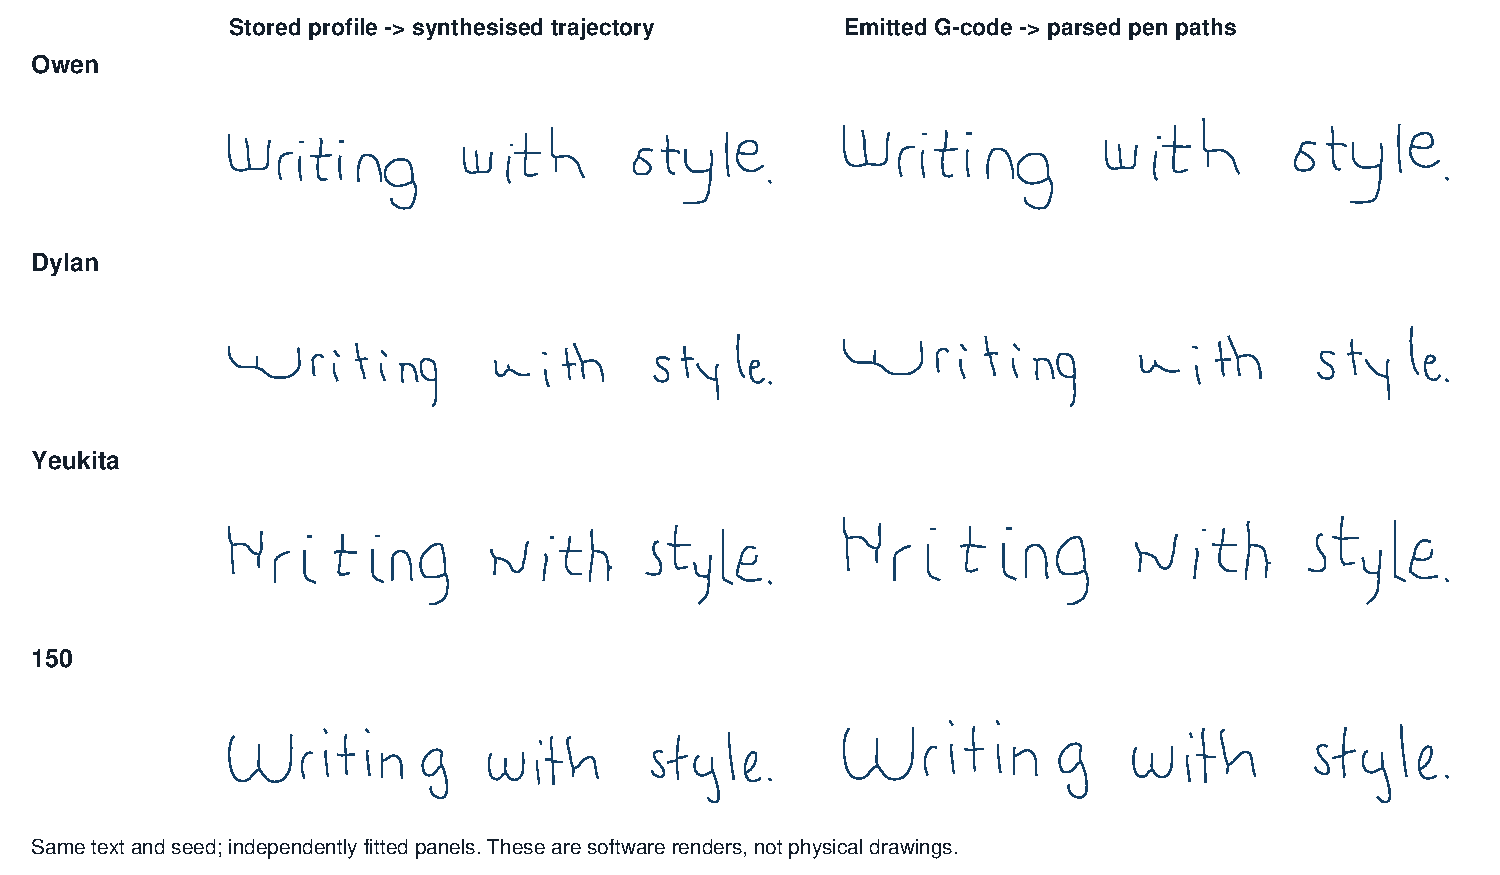
\includegraphics[width=0.98\linewidth]{Figures/design-style-gcode-examples.pdf}
\caption{Same text generated from four final profiles and reconstructed from emitted G-code. These are software path drawings.}
\label{fig:des-style-files}
\end{figure}

Algorithm~\ref{alg:des-file-reference} describes the serialization check. Nine controlled fixtures combined scale factors 1, 3 and 30 with line offsets 0, 8.4 and 25.2\,mm. Ring closure and joining were disabled, minimum-segment filtering was set to zero, and the independently parsed paths were paired with \texttt{ToMachine}'s output. Each fixture retained path and vertex counts, with no clamped points. Maximum coordinate error was $0.0004$\,mm, within the $0.0005$\,mm per-coordinate rounding bound from three-decimal emission. This comparison checks serialization after placement; it does not independently prove that the placement equation itself is correct or that a motor reached a coordinate.

\begin{designalgorithm}
\caption{Controlled G-code serialization correspondence}
\label{alg:des-file-reference}
\prequire{Known multi-path trajectory and configurations with joins and closure disabled.}
\begin{designpseudo}
\pstate{0}{\textbf{for each} fixture configuration $c$ \textbf{do}}
\pstate{1}{$P\leftarrow\operatorname{ToMachine}(T,c)$}
\pstate{1}{$f\leftarrow\operatorname{WriteGcode}(T,c)$; $Q\leftarrow\operatorname{ParseGcode}(f)$}
\pstate{1}{Compare path counts and corresponding vertex counts}
\pstate{1}{Record $\max_i\|P_i-Q_i\|_\infty$ and clamped-point count}
\pstate{0}{\textbf{end for}}
\pstate{0}{\textbf{return} count agreements, rounding discrepancies and clipping records}
\end{designpseudo}
\end{designalgorithm}

Figure~\ref{fig:des-physical-page} is separately identified as a photograph of actual robot output, from the existing Owen reproduction sheet. The line crops are newly obtained from that stored photograph. This closes the visual explanation from a physical page to the segmentation interface, without presenting the earlier drawing as a newly executed hardware experiment. No exact same-job correspondence with Figure~\ref{fig:des-style-files} is claimed.

\begin{figure}[!htbp]\centering
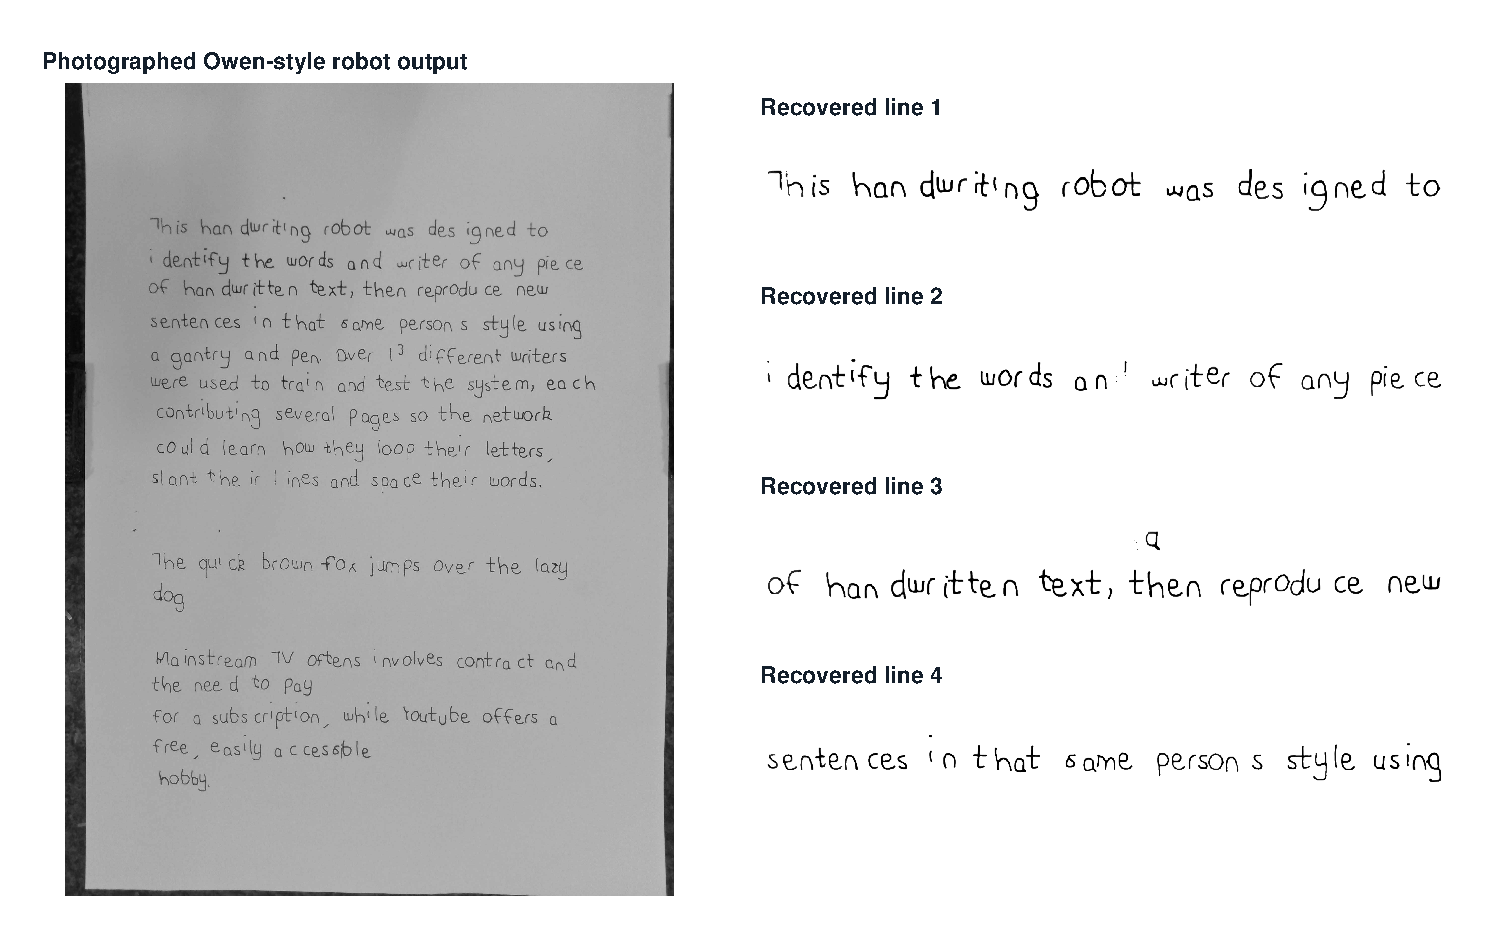
\includegraphics[width=0.95\linewidth]{Figures/design-physical-page-example.pdf}
\caption{Existing photographed robot output and newly recovered line crops. The photograph is distinct from the software renders above.}
\label{fig:des-physical-page}
\end{figure}

\subsection{Candidate-scoring configuration and scope}
The Owen trials use the joint reader and eleven-writer \texttt{pw170} checkpoint, with explicit 0.17 normalisation and uniform-ink rendering. They score character accuracy and requested-writer posterior before repair, independently of inherited server defaults. Exact inputs, readings and full-precision scores are retained in \texttt{Evidence/bench.json}.

\subsection{Post-design seam-coefficient sensitivity}
\label{app:des-seam-sweep}
A new one-at-a-time check examines the existing seam weights. Owen01 and Yeukita01 are reduced to a maximum dimension of 1600 pixels, then passed through orientation, conditioning and line-centre estimation. The first, middle and last gaps on each page are selected by index before inspecting outputs. Eight settings share these six gaps, step limit seven and ink weight four: midpoint weight varies at step penalty 0.02, then step penalty varies at midpoint weight 0.012. This is post-design sensitivity, not a joint search or recovered historical tuning.

The parameterised reference matches all six unmodified default paths. Table~\ref{tab:app-seam-sweep} reports raw-ink intersections, total row movement and mean midpoint distance in working pixels; the midpoint is a preference, not a labelled correct boundary.

\begin{table}[!htbp]\centering\small
\begin{tabular}{|c|c|r|r|r|}
\hline Midpoint weight&Step penalty&Ink intersections&Row movement&Mean offset / px\\\hline
0.000&0.020&2&35&4.0553\\\hline
0.006&0.020&2&38&0.5517\\\hline
0.012&0.020&2&42&0.3625\\\hline
0.024&0.020&2&44&0.3261\\\hline
0.048&0.020&2&47&0.2622\\\hline
0.012&0.000&2&48&0.2622\\\hline
0.012&0.010&2&44&0.3261\\\hline
0.012&0.040&2&38&0.5517\\\hline
\end{tabular}
\caption{New coefficient-sensitivity check across six fixed real-page gaps; the implemented setting is 0.012/0.020.}
\label{tab:app-seam-sweep}
\end{table}

Increasing midpoint weight from zero to 0.012 reduces mean offset from 4.055 to 0.363 pixels, while row movement rises from 35 to 42 pixels. Doubling the weight gives 0.326 pixels offset. Increasing step penalty has the opposite trade-off. Every setting retains two raw-mask and three closed-mask intersections. These cases therefore show competing effects without establishing a unique optimum, eliminating intersections or measuring recognition accuracy. Input/code hashes and all 48 runs are supplied; no pipeline coefficient was changed.
\FloatBarrier

\subsection{Real-input calculation traces}\label{app:des-real-calculations}
The numerical substitutions in Design were captured from offline processing of existing project inputs. They are execution traces of the stated calculations, not reconstructed historical training decisions or measurements of the mechanism. The complete settings, input/model hashes and full-precision values are stored in \texttt{Evidence/real\_calculations.json}; \texttt{trace\_real\_calculations.py} reproduces them without changing model weights or final profiles.

The page-conditioning trace uses Owen01 reduced to 1600 rows by 1200 columns, giving an 800-row by 600-column working image before deskew. The network and extraction trace instead uses the separately identified archived first original Owen01 crop ($156\times2170$), its known transcript and the joint reader. The latter produces $160\times1\times75$ log probabilities: the checkpoint head has 75 rows, consistent with 74 alphabet symbols and blank. The selected eleven-writer model uses explicit 0.17-width preparation for the two-crop vote. These inputs must not be mistaken for one continuous new whole-system test.

For the first convolution calculation, the actual input patch and learned kernel, listed in the same row-major order, are
\[
X=\begin{bmatrix}-1&-1&-1\\-0.552941&-0.380392&-0.568627\\0.866667&0.960784&0.866667\end{bmatrix},\qquad
W=\begin{bmatrix}0.213027&-0.215063&0.234474\\0.068398&0.083297&0.187499\\-0.312354&-0.291350&-0.221197\end{bmatrix}.
\]
Using the full-precision values with bias $-0.000435125$ gives $-1.15133214$ at output channel 0, row 34, column 462. Rounded values above explain the sum; the manifest retains the precise arrays needed to reproduce it. The subsequent batch-normalisation and LSTM substitutions follow this same crop through the reader.

The path and timing trace generates ``Writing with style.'' using the final Owen profile, seed 2026, requested x-height 4\,mm and jitter 0.15. The generated file is \texttt{Evidence/real\_trace\_owen.gcode}. Its default configuration supplies drawing/travel feeds 900/2400\,mm/min, nominal conversion 80 microsteps/mm and the 190.6 by 251.3\,mm workspace. No physical command was sent. The pulse-delay calculation uses one emitted segment at that nominal scale; actual homing counts remain a separate hardware measurement. The trace also records the pre-file coordinate mapping, distance accumulators, 56 pen transitions and the resulting 32.8\,s nominal budget.

The existing random-mask, exhaustive seam and small-lattice checks remain independent numerical tests. Their synthetic inputs are intentional test fixtures. They are separate from these real-input traces and from the qualification results.

\clearpage
\subsection{Visual checks of numerical training operations}\label{app:vt-gradient}
The retained visual-test record contains 249 scalar perturbation comparisons: 73 sampled convolution-weight entries, 73 bias comparisons, 73 input entries and all 30 logits of a small CTC lattice. The sampled entries need not be distinct parameters. Central differences use a step of $10^{-6}$ for the convolution and $10^{-5}$ for CTC, following the numerical-check principle in Equation~\ref{eq:des-gradcheck}. Figure~\ref{fig:vt-grad} compares the resulting numerical derivatives with the implemented backward operations. Relative difference is the absolute discrepancy divided by the sum of the two derivative magnitudes, with a $10^{-12}$ denominator floor.

The largest relative difference is $7.50\times10^{-7}$, among the sampled convolution inputs; the largest absolute input discrepancy is $7.26\times10^{-9}$. The CTC relative difference is at most $1.69\times10^{-9}$. These checks support the tested local derivatives under the fixed fixtures. They do not exercise every layer, parameter, floating-point regime or complete training run.

\begin{figure}[!htbp]\centering
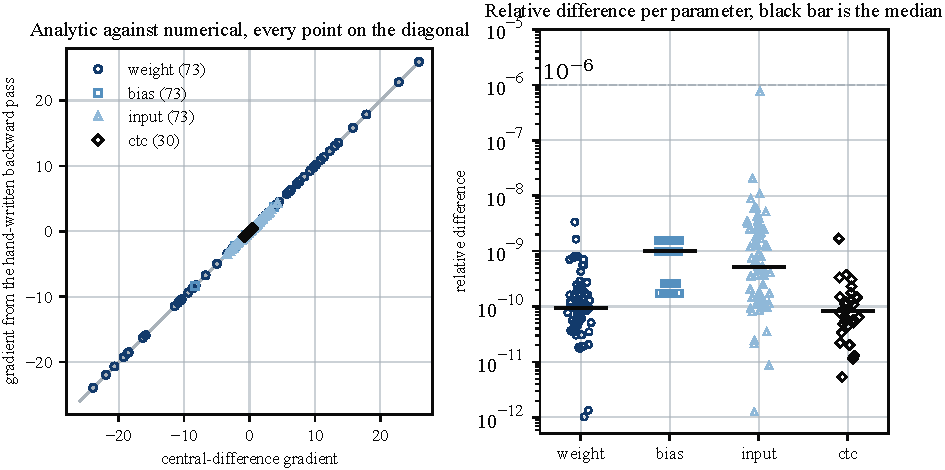
\includegraphics[width=\linewidth]{Figures/VisualTests/T38_gradient_check.pdf}
\caption{Analytic and central-difference gradients for sampled convolution quantities and a complete small CTC logit array.}
\label{fig:vt-grad}
\end{figure}

\subsection{Stroke-width quantisation in the validation sweep}\label{app:vt-width}
Figure~\ref{fig:vt-width} shows four real crops processed at the four sweep fractions. The image transformation depends on the resulting odd integer dilation kernel as well as the fraction. For Owen and Abhinav, 0.06 and 0.09 both select $k=3$ on the illustrated crop; for Dylan, 0.09 and 0.11 both select $k=5$. Identical kernels give identical normalised images for that same crop. This does not imply that two settings produce identical training datasets, since x-height varies across crops. The validation bars reproduce the supplied training sweep, not a new accuracy measurement. Its best observed setting remains 0.17, while a single run at each setting does not isolate width effects from training variability.

\begin{figure}[!htbp]\centering
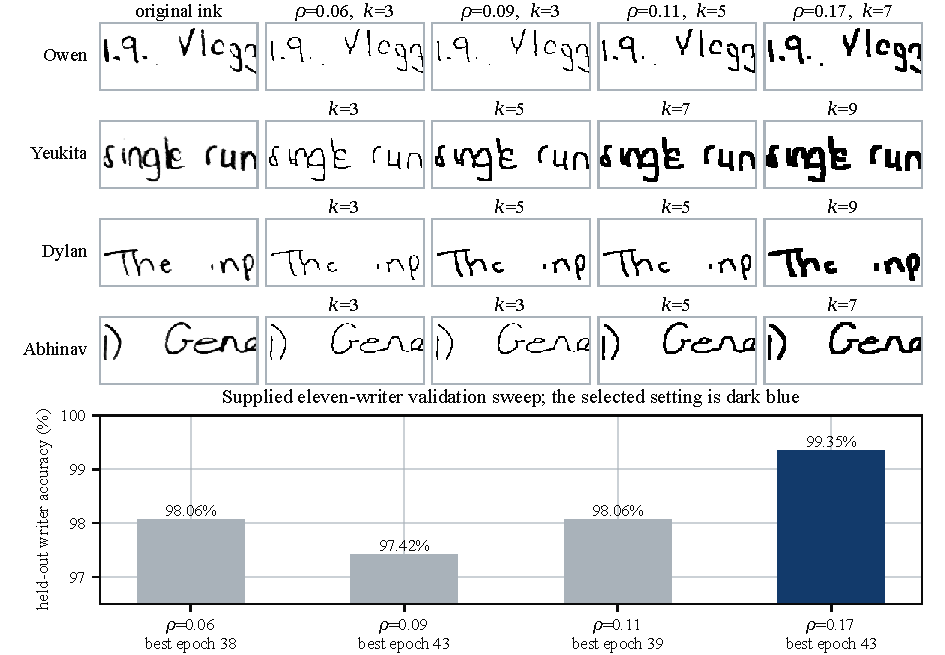
\includegraphics[width=\linewidth]{Figures/VisualTests/T40_stroke_width_sweep.pdf}
\caption{Real-crop normalisation kernels alongside the previously reported eleven-writer validation sweep.}
\label{fig:vt-width}
\end{figure}

\subsection{Glyph coordinates and measured connectedness}\label{app:vt-glyphgeometry}
Figure~\ref{fig:vt-coordinates} shows the actual Owen \texttt{V} used in the coordinate calculation in Design: left boundary 146 pixels, baseline 107 pixels, x-height 38 pixels and slant $-4.5^\circ$. The stored path uses the baseline as its origin, measures height upwards and expresses lengths in x-heights. The lead is stored separately from the path so that source-cell spacing is not confused with the first surviving ink point.

\begin{figure}[!htbp]\centering
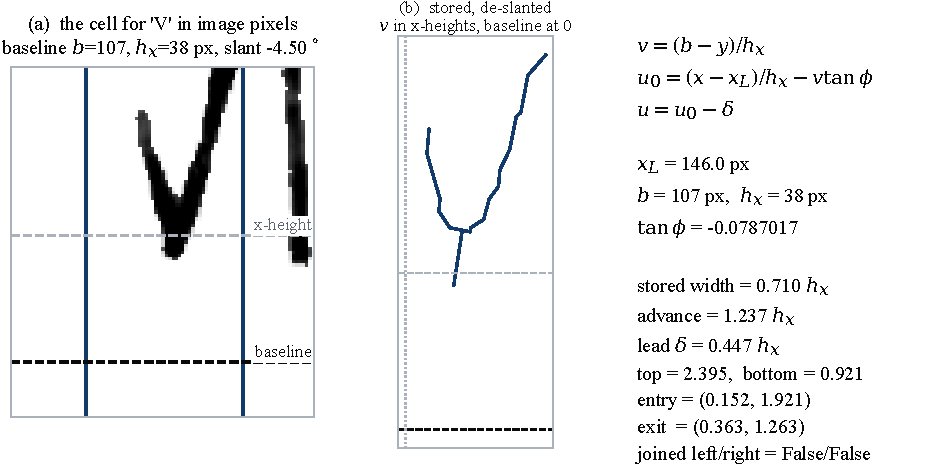
\includegraphics[width=\linewidth]{Figures/VisualTests/T43_glyph_coordinates.pdf}
\caption{The same glyph in image coordinates and in its stored, de-slanted coordinate frame.}
\label{fig:vt-coordinates}
\end{figure}

Figure~\ref{fig:vt-connectedness} makes the connectedness definition inspectable on the same line. Three of its 39 eligible adjacent non-space boundaries are crossed by a traced centreline, giving $3/39=0.076923$. This is the line-level example already used in Design. A crossing records connected source ink under the extraction convention; it does not reveal the writer's natural pen-lift sequence or establish a connection fraction for every page by itself.

\begin{figure}[!htbp]\centering
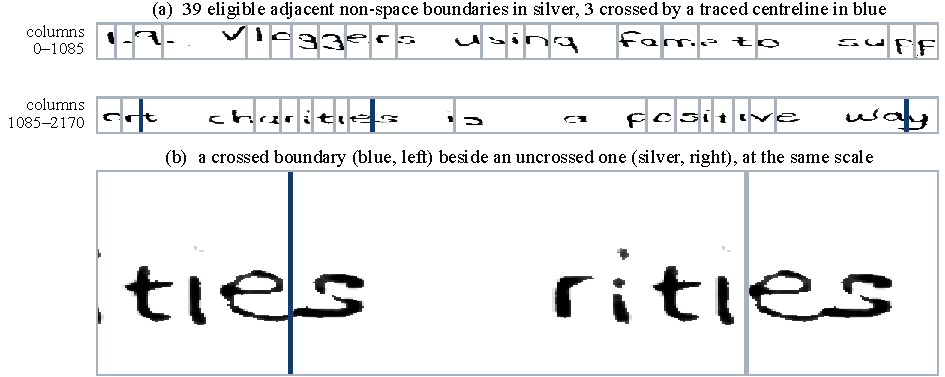
\includegraphics[width=\linewidth]{Figures/VisualTests/T49_connectedness.pdf}
\caption{Eligible character boundaries and the three observed centreline crossings in one original line.}
\label{fig:vt-connectedness}
\end{figure}

\FloatBarrier

\clearpage
\section{Supporting qualification evidence}
\label{app:res-evidence}
This appendix preserves the detail needed to interpret the main qualification tests without repeating the Design's subsystem derivations. The source package contains the original v6 measurement archive, the reviewed aggregate records and the scripts that generate the revised tables and figures. Newly computed analyses are identified separately from the original measurements. No physical measurement is generated by a plotting script.

\subsection{Evaluated checkpoints and populations}
The selected demonstration reader is the library-trained joint reader, as confirmed by the author. The numerical scratch reader is a comparison model. The selected writer model is the library-trained eleven-writer 0.17 model. Table~\ref{tab:app-checkpoints} records hash prefixes; the evidence manifest retains the full SHA-256 values. A filename alone is insufficient because the archived reader study identified two different files named \texttt{scratch\_best}.

\begin{table}[!htbp]\centering\small
\begin{tabular}{lll}\toprule
\textbf{Role} & \textbf{Checkpoint identifier} & \textbf{SHA-256 prefix}\\\midrule
Selected reader & joint\_best & \texttt{336802d535992323}\\
Comparison reader & evaluated scratch\_best & \texttt{2add315ded078de5}\\
Selected writer & 11\_pw170 & \texttt{1884fb86467538eb}\\
Comparison writer & 11w\_pw170\_scratch & \texttt{b23a709a30144f67}\\\bottomrule
\end{tabular}
\caption{Identities of the measured model files.}\label{tab:app-checkpoints}\end{table}

The numerical-writer training excerpt supplied by the author records 1\,031 training lines and 155 validation lines, 0.17 normalisation, a 50-epoch budget and a best displayed validation accuracy of 0.968 by epoch 41. The retained excerpt continues through epoch 47 and does not document a completed epoch 50. Its later common-set score is measured on 156 re-extracted validation lines; the different population is retained rather than silently equated with training validation. The numerical-reader excerpt records 6\,481 public training lines, 569 personal training lines, 976 public validation lines and 100 personal validation lines, and a resume from an existing checkpoint. These are training-history records, while QT~2 evaluates saved weights directly.

An additional inventory reads each selected stored profile and verifies nonempty glyph mappings. The numbers of distinct character keys are 42, 38, 37, 36, 40 and 41 for the six database writers, and 56, 42, 43, 42 and 58 for A, B, O, T and Y. All eleven names agree with the selected writer checkpoint. The full source paths and content hashes are preserved in \texttt{ResultsEvidence/profile\_inventory.json}. These counts establish stored mappings; they do not imply equal coverage of every character in the reader alphabet.

\subsection{Physical reproduction by writer}
\begin{table}[!htbp]\centering\small
\begin{tabular}{lrrrr}\toprule
\textbf{Writer} & \textbf{Lines} & \textbf{Character / \%} & \textbf{Writer / \%} & \textbf{Word match / \%}\\\midrule
Y & 13 & 97.01 & 92.31 & 74.16\\
150 & 13 & 96.75 & 53.85 & 76.40\\
O & 16 & 94.25 & 100.00 & 58.51\\
B & 16 & 93.11 & 93.75 & 68.24\\
384 & 16 & 86.93 & 87.50 & 43.18\\
552 & 15 & 86.17 & 80.00 & 48.39\\
152 & 15 & 85.74 & 80.00 & 49.44\\
A & 27 & 77.29 & 100.00 & 18.09\\
153 & 19 & 75.72 & 57.89 & 31.46\\
588 & 18 & 73.19 & 94.44 & 22.99\\
T & 16 & 60.97 & 100.00 & 13.41\\
\bottomrule\end{tabular}
\caption{Full per-writer reproduction results on 184 labelled lines. Word match uses equal word positions and is not one minus word edit error rate.}\label{tab:app-r1-writers}
\end{table}

The paired read-back study contains 184 transcript-bearing lines. A separate model comparison contains 185 writer-labelled crops, including one crop with no corresponding transcript line. It can support a writer-prediction comparison, but that extra crop is not inserted into a character score. The model-comparison pooled groups are writers, not a claim that only eleven physical sheets were drawn.

\subsection{New geometric style comparison on physical pages}
\label{app:res-physical-style}
The new analysis applies the archived descriptor definitions with the current segmentation primitives to 156 original reference lines and 184 physical-output lines. The original population consists of the same six held-out database pages and 100 seeded photographed reference lines used for writer evaluation. The physical population comprises all fourteen robot pages after the recorded orientation convention. Each page's crop count agrees with its transcript-bearing records, and every line returns usable descriptors. All eleven writers are retained.

Each line is binarised, its body band estimated and its image resized toward a 28-pixel body height before the descriptors are evaluated. The same procedure is applied to both domains. Writer means give equal weight to available lines for each feature, and the pooled correlation gives equal weight to writers and selected features. Word-gap values are absent where no qualifying gap exists: 155/156 original and 180/184 physical lines have a value; the other descriptors are available for every line. All eleven writer means remain usable. The within-domain variant separately standardises each feature in each domain; the absolute variant uses original-domain means and standard deviations for both. Source images, the personal-crop cache, scripts and full measurements are recorded by hash. The raw outputs are in \texttt{ResultsEvidence/physical\_style/results.json}.

The per-feature correlations are slant 0.9911; stroke width 0.7986; ink density 0.7392; word gap 0.4861; components per word 0.6688; character width 0.7978; ascender extent 0.8173; descender extent 0.5394; and extent ratio 0.5762. Figure~\ref{fig:app-physical-style} shows the actual writer means. The 10\,000-repeat writer-resampling range for the seven-feature within-domain coefficient is 0.5555--0.8272, using seed 23539195. It is a sensitivity range over this writer set. This retrospective comparison does not use identical sentences between domains and should not be interpreted as a controlled perceptual-equivalence experiment.
\begin{figure}[!htbp]\centering
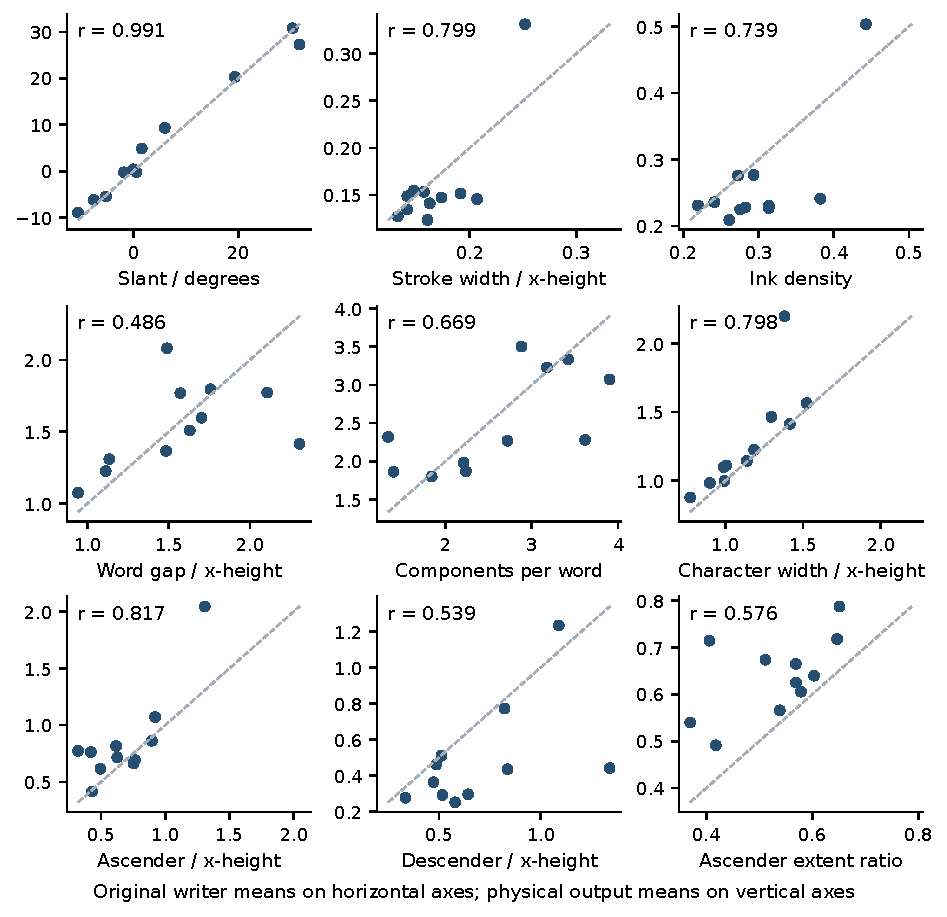
\includegraphics[width=0.99\linewidth]{Figures/results_physical_style_scatter.pdf}
\caption{New physical-to-original style descriptors across eleven writers. Each point is one writer mean. Dashed lines indicate equal values; correlation can remain high even when magnitudes differ.}\label{fig:app-physical-style}\end{figure}

\subsection{Archived geometric style study}
\label{app:res-style}
The archived study covers writers 150, 151, 152, 153, 384, 551, 552, 588, B and Y. There are six synthetic lines per writer, sixty in total, compared with 123 original reference lines marked as excluded from profile building. This earlier ten-writer set differs from the final eleven-writer evaluation. The study is retained to explain geometric behaviour of the method; it is not relabelled as a measurement of final physical pages.

Nine deterministic descriptors measure slant, normalised stroke width, ink density, word gap, components per word, character width, ascender extent, descender extent and the ascender-to-total-extent ratio. Seven shape descriptors omit stroke width and ink density. The within-domain pooled correlation first standardises each feature across writers separately in the real and synthetic domains, then correlates the flattened arrays. It is therefore insensitive to a uniform offset or scale difference between those domains. The alternative absolute variant standardises both arrays using the real-domain mean and standard deviation. This distinction matters when interpreting preservation of magnitude rather than writer ordering.

\begin{table}[!htbp]\centering\small
\begin{tabular}{lrr}\toprule
\textbf{Feature set} & \textbf{Separate-domain standardisation} & \textbf{Real-domain standardisation}\\\midrule
Nine features & 0.7013 & 0.5994\\
Seven shape features & 0.7142 & 0.6711\\\bottomrule
\end{tabular}
\caption{Archived synthetic-to-original pooled correlations against the profile-held-out reference. The 0.714 value is the seven-shape-feature variant.}\label{tab:app-style-variants}\end{table}

The per-feature coefficients are 0.9964 for slant, 0.6315 for stroke width, 0.6802 for ink density, 0.6050 for word gap, 0.8323 for components per word, 0.9358 for character width, 0.9735 for ascender extent, 0.1480 for descender extent and 0.5085 for the extent ratio. Correlation describes variation across writers; it does not prove pointwise agreement of all letter shapes. The recorded 2\,000 writer-resample interval for the seven-feature within-domain result is 0.6118--0.8586.

The archived overlay experiment uses thirty source texts across those ten writers. With x-height normalisation, mean matched chamfer distance is 0.6302, mean mismatched distance is 1.3868, their ratio is 2.2007 and the recorded AUC is 0.7074. When the archive also applies its width-normalisation variant, AUC is 0.4630. Thus the favourable separation depends on the chosen normalisation; an AUC above 0.5 in one variant must not be presented as universal writer fidelity. These remain software comparisons, without a new independent human panel.

\subsection{Timing selection and optimisation scope}
\label{app:res-speed}
QT~3 uses a deliberately checkable completion boundary. The earlier archive retained 36 records after deduplication and a drawing-rate filter. The revised primary count uses 25 positive-character console records with explicit program-end evidence. The original 36-record aggregation remains in the preserved provenance document. A rate threshold alone does not establish completion: a job stopped after substantial drawing can exceed that threshold. This change does not alter the observed worst 3.875~s per character. A terminal marker confirms the interpreter finished, while geometry and content remain separate qualification questions.

The 500- and 982-character counts for QT~4 are the counts printed in the timer record. A final repeat should retain independent transcript lengths and an acquisition-to-output timing boundary. The two current overruns are large, so no inferred sub-second camera transfer time is added to create a favourable pass.

\begin{table}[!htbp]\centering\small
\begin{tabularx}{\linewidth}{lX}\toprule
\textbf{Comparison} & \textbf{Measured outcome and scope}\\\midrule
Sequential NumPy vs batched library networks & 359.8~s vs 130.3~s over fourteen stored pages on the development host; factor 2.76. Both backend and batching change. Reader text is identical; writer-label equivalence is not inferred from that fact.\\[4pt]
Full vs half linear image resolution & 4.37-fold recorded image-stage factor on comparable successful page pairs, with 247 vs 182 detected lines. Zero of twelve comparable pages retain line count; two of fourteen reduced pages fail segmentation.\\[4pt]
Projected network-only replacement & Applying 2.76 to ODROID network stages, with image stages unchanged, gives approximately 27.05~s and 30.82~s. Neither is an observed ODROID result or a total-time pass.\\[4pt]
Projected combined replacement & Applying both host factors gives approximately 14.61~s and 17.86~s. The second is numerically below its allowance, but the image reduction changes the output and the timing is transferred between hosts. It is not accepted as R4 compliance.\\\bottomrule
\end{tabularx}
\caption{Acceleration evidence and the boundary between a measured comparison and a projected compliant configuration.}\label{tab:app-acceleration}\end{table}

The G-code study of the same 378-character paragraph yields pen-down path lengths from 2\,015.4 to 3\,942.8~mm and recorded pen-state counts from 544 to 1\,188 across eleven profiles. These are arithmetic properties of generated paths. They demonstrate profile-dependent geometry and help explain timing variation; they are not independent proof of similarity to genuine handwriting, and their values can still be affected by the candidate-selection process.

\subsection{Cost, consent and final records}
The photographed ledger supplied by the author is retained as evidence. The present build estimate is approximately R4\,000, with a borrowed ODROID entered at zero purchase cost. The later listed clipboard (R90), paper (R130), gel pen (R30) and estimated training electricity (R500) total R750. Their overlap with the approximate build estimate is not established, so they are not added to produce an unsupported exact total. Replacement value and estimated operating costs should be distinguished from actual purchased parts.

Signed consent forms are held by the author for the five personal contributors. The report records that fact without reproducing signatures. Participant consent is recorded separately from institutional clearance or exemption.

\subsection{Supporting timing and dimensional figures}
\begin{figure}[!htbp]\centering
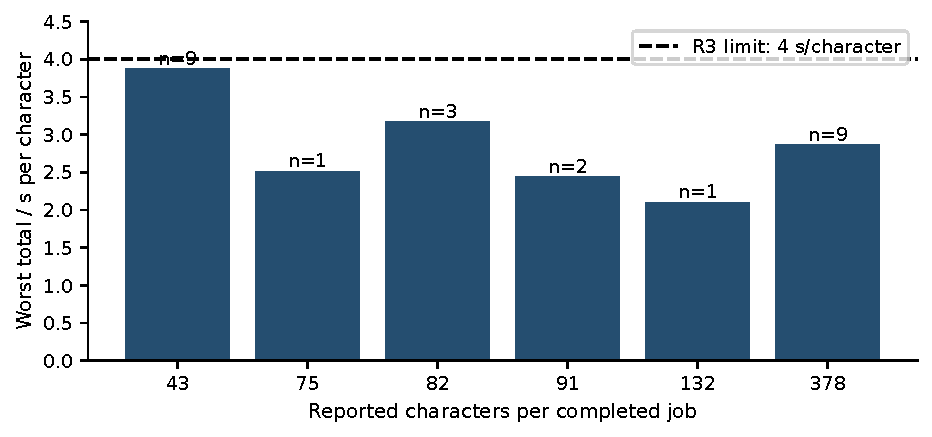
\includegraphics[width=0.98\linewidth]{Figures/results_r3_confirmed.pdf}
\caption{Worst recorded generation-plus-drawing time at each tested length, using only explicitly completed jobs. Labels state the number of records. The timing result applies to these recorded jobs and does not imply identical quality for every writer.}
\label{fig:res-r3}\end{figure}
\begin{figure}[!htbp]\centering
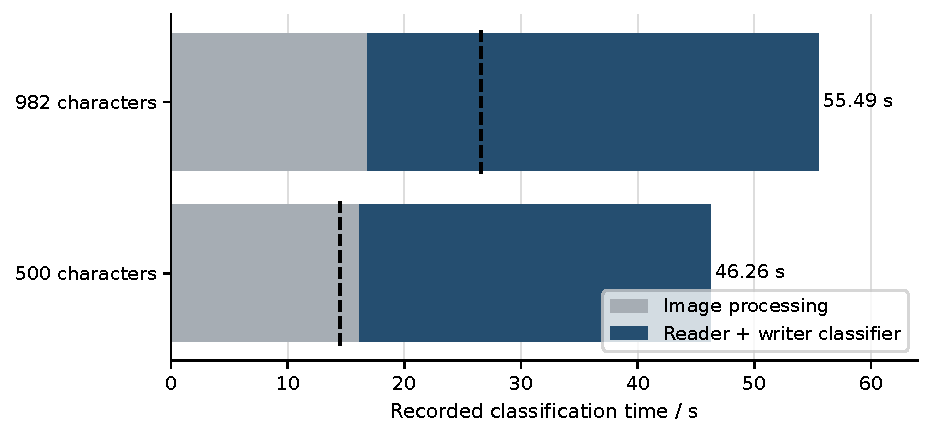
\includegraphics[width=0.98\linewidth]{Figures/results_r4_stages.pdf}
\caption{Recorded ODROID classification time split into image and network stages. Dashed markers show the complete R4 allowance at each logged character count. Both measured totals exceed their allowance.}
\label{fig:res-r4}\end{figure}
\begin{figure}[!htbp]\centering
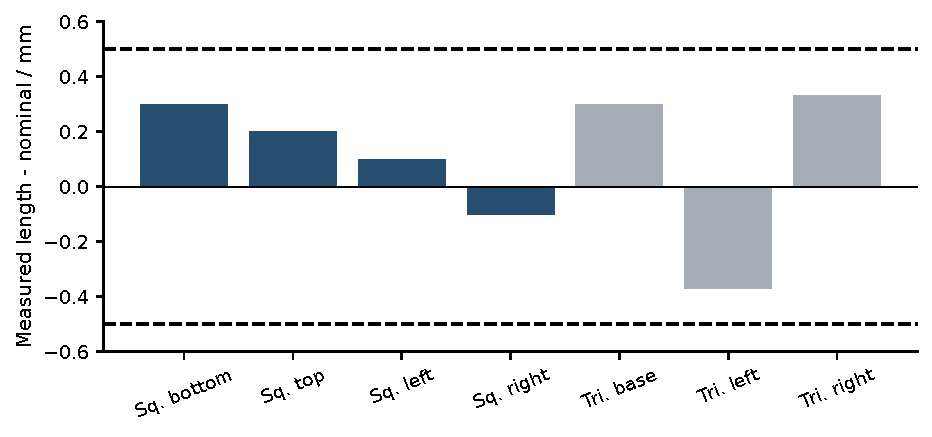
\includegraphics[width=0.98\linewidth]{Figures/results_geometry_errors.pdf}
\caption{Signed dimensional differences for one square and one triangle. Dashed lines are the 0.5~mm reference. Being inside those lines is a feature-length observation, not an absolute coordinate-error bound over the bed.}
\label{fig:res-geometry}\end{figure}

\end{document}
